\documentclass[11pt,a4paper,oneside,openany,indonesian]{report}
\usepackage[a4paper,top=25mm,bottom=25mm,left=30mm,right=25mm,headheight=16pt,headsep=7mm,footskip=12mm]{geometry}
\usepackage{iftex}
\ifLuaTeX
  \usepackage[bidi=basic,shorthands=off,provide=*]{babel}
\else
  \usepackage[bidi=default,shorthands=off,provide=*]{babel}
\fi
\ifPDFTeX\else\babelfont{rm}[]{Times New Roman}\fi
\usepackage{hyperref}
% Shared preamble for the Jakarta TGA chapters.
\usepackage{xcolor}
\usepackage{graphicx}
\usepackage{amsmath,amssymb}
\usepackage{iftex}
\ifPDFTeX
  \usepackage[T1]{fontenc}
  \usepackage[utf8]{inputenc}
  \usepackage{textcomp}
\else
  \usepackage{unicode-math}
  \defaultfontfeatures{Scale=MatchLowercase}
  \defaultfontfeatures[\rmfamily]{Ligatures=TeX,Scale=1}
\fi
\usepackage{lmodern}
\ifPDFTeX\else
  \setmainfont[]{Times New Roman}
  \setsansfont[]{Arial}
  \IfFontExistsTF{Consolas}{\setmonofont[]{Consolas}}{\setmonofont[]{Courier New}}
\fi
\IfFileExists{microtype.sty}{\usepackage{microtype}}{}
\usepackage{longtable,booktabs,array,tabularx,adjustbox,calc}
\usepackage{pdflscape}
\usepackage{caption}
\captionsetup[table]{skip=6pt}
\newcounter{none}
\usepackage{float}
\usepackage{setspace}
\usepackage{ragged2e}
\usepackage{titlesec}
\usepackage{enumitem}
\usepackage{needspace}
\usepackage{fancyhdr}
\usepackage{newunicodechar}
\usepackage{bookmark}
\usepackage{xurl}
\usepackage{csquotes}
\usepackage[backend=biber,style=authoryear,maxcitenames=2,maxbibnames=99,uniquelist=false,uniquename=false]{biblatex}
\DeclareLanguageMapping{indonesian}{english}
\DefineBibliographyStrings{english}{and={dan},andothers={dkk\adddot}}
\DefineBibliographyStrings{indonesian}{and={dan},andothers={dkk\adddot}}
\AtBeginDocument{\renewcommand*{\finalnamedelim}{\addspace dan\space}}
\addbibresource{references.bib}
\DeclareFieldFormat{title}{#1}
\DeclareFieldFormat[article,inbook,incollection,inproceedings,inreference,patent,thesis,unpublished]{title}{#1}
\AtBeginBibliography{\small\setlength{\bibitemsep}{0.15em}}

\newunicodechar{∅}{\ensuremath{\varnothing}}

% Placeholder untuk gambar yang dibuat manual (peta GIS). Ganti dengan \includegraphics setelah berkas target tersedia.
\newcommand{\GambarPlaceholder}[2][7cm]{%
  \fbox{\parbox[c][#1][c]{0.92\linewidth}{\centering\small
    \textbf{PLACEHOLDER GAMBAR}\\[0.6em]#2}}}

\definecolor{Ink}{HTML}{222222}
\definecolor{RuleGray}{HTML}{666666}

\AtBeginDocument{%
  \hypersetup{linkcolor=Ink,citecolor=Ink,urlcolor=Ink,pdfborder={0 0 0}}%
  \urlstyle{same}%
}

\setstretch{1.5}
\setlength{\parindent}{1.1em}
\setlength{\parskip}{0.28em}
\setlength{\emergencystretch}{2.5em}
\clubpenalty=10000
\widowpenalty=10000
\displaywidowpenalty=10000
\raggedbottom

\setlist[itemize]{leftmargin=1.7em,itemsep=0.25em,topsep=0.35em}
\setlist[enumerate]{leftmargin=1.9em,itemsep=0.25em,topsep=0.35em}

\titleformat{\chapter}[display]
  {\normalfont\bfseries\centering\color{Ink}}
  {}{0pt}{\Large\hyphenpenalty=10000\exhyphenpenalty=10000}
\titlespacing*{\chapter}{0pt}{-6pt}{18pt}
\titleformat{\section}{\Needspace{4\baselineskip}\large\bfseries\color{Ink}}{\thesection}{0.7em}{}
\titleformat{\subsection}{\Needspace{3\baselineskip}\normalsize\bfseries\color{Ink}}{\thesubsection}{0.7em}{}
\titleformat{\subsubsection}{\Needspace{3\baselineskip}\normalsize\bfseries\color{Ink}}{\thesubsubsection}{0.7em}{}

\pagestyle{plain}
\fancyhf{}
\fancyfoot[C]{\thepage}
\renewcommand{\headrulewidth}{0pt}
\renewcommand{\footrulewidth}{0pt}
\fancypagestyle{plain}{%
  \fancyhf{}
  \fancyfoot[C]{\thepage}
  \renewcommand{\headrulewidth}{0pt}
}

\renewcommand{\arraystretch}{1.2}
\setlength{\extrarowheight}{1pt}
\setlength{\tabcolsep}{4pt}
\providecommand{\tightlist}{\setlength{\itemsep}{0pt}\setlength{\parskip}{0pt}}
\setlength{\LTpre}{0.5em}
\setlength{\LTpost}{0.8em}
\AtBeginEnvironment{longtable}{\footnotesize\setstretch{1.0}\setlength{\tabcolsep}{3pt}\setlength{\extrarowheight}{1pt}}
\AtBeginEnvironment{table}{\setstretch{1.0}}
\AtBeginEnvironment{figure}{\setstretch{1.0}}
\AtBeginEnvironment{quote}{\small\setlength{\leftskip}{1.2em}\setlength{\rightskip}{1.2em}}

\graphicspath{{figures/}}

\hypersetup{
  pdftitle={TGA PWK Jakarta - Bab 1--4},
  pdfauthor={Mahastri Laksita Sam Widita},
  pdflang={id-ID},
  hidelinks
}

\title{\textbf{Borrowed Size atau Agglomeration Shadow?}\\[0.4em]
Analisis Hubungan Integrasi Metropolitan dengan Kematangan Pusat-Pusat Sekunder Jabodetabek}
\providecommand{\subtitle}[1]{\gdef\thesubtitle{#1}}
\subtitle{Naskah Bab 1--4}
\author{Mahastri Laksita Sam Widita}
\newcommand{\studentnumber}{22/503065/TK/54947}
\newcommand{\advisorname}{Rendy Bayu Aditya}
\date{Kabupaten Sleman, Daerah Istimewa Yogyakarta\\2026}

\makeatletter
\renewcommand{\maketitle}{%
  \begin{titlepage}
    \centering
    \vspace*{0.8cm}
    {\Large \@title\par}
    \vspace{0.55cm}
    {\Large\bfseries TUGAS AKHIR\par}
    \vspace{0.25cm}
    {\normalsize \thesubtitle\par}
    \vspace{0.3cm}
    {\normalsize Program Studi Perencanaan Wilayah dan Kota\par}
    \vspace{0.65cm}
    {\normalsize Disusun sebagai salah satu persyaratan akademik pada Program Studi\\
      Perencanaan Wilayah dan Kota\par}
    \vspace{0.55cm}
    
\includegraphics[width=4.4cm]{lambang_ugm_hitam.png}\par
    \vspace{0.45cm}
    {\normalsize\@author\par}
    \vspace{0.15cm}
    {\normalsize NIM \studentnumber\par}
    {\normalsize Pembimbing: \advisorname\par}
    \vfill
    {\normalsize\bfseries
      PROGRAM STUDI PERENCANAAN WILAYAH DAN KOTA\\
      DEPARTEMEN TEKNIK ARSITEKTUR DAN PERENCANAAN\\
      FAKULTAS TEKNIK\\
      UNIVERSITAS GADJAH MADA\par}
    \vspace{0.45cm}
    {\normalsize \@date\par}
  \end{titlepage}}
\makeatother

\begin{document}
\maketitle
\tableofcontents
\clearpage

\chapter{Bab 1 Pendahuluan}

\section{Latar belakang}

Perkembangan metropolitan Jakarta tidak berhenti pada batas administratif DKI Jakarta.\footnote{Undang-Undang Nomor 2 Tahun 2024 mengubah nama provinsi menjadi Provinsi Daerah Khusus Jakarta. Pasal 73 undang-undang tersebut mengaitkan saat berlakunya dengan penetapan Keputusan Presiden mengenai pemindahan ibu kota negara \parencite{uu22024}. Seluruh publikasi statistik yang dipakai, sampai \emph{Provinsi DKI Jakarta Dalam Angka 2026}, masih memakai nama ``DKI Jakarta''. Naskah ini karena itu memakai ``DKI Jakarta'' sebagai nama wilayah statistik.} Permukiman, kawasan industri, pusat pelayanan, dan jaringan transportasi berkembang di wilayah sekitarnya, sementara perjalanan penduduk dan kegiatan ekonomi menghubungkan berbagai bagian kawasan tersebut. Jakarta tetap menjadi pusat dominan, tetapi sejumlah kawasan di sekitarnya telah menjadi konsentrasi penduduk, pekerjaan, industri, dan pelayanan. Kajian mengenai Jabotabek dan Jabodetabek mencatat pergeseran kegiatan ke pinggiran, perkembangan kota baru dan kawasan industri, serta arus komuter antarpinggiran \parencite{henderson1996,hudalahfirman2012,hudalahetal2013,sadewoetal2023}.

Hubungan tersebut kini juga menjadi persoalan kebijakan. Undang-Undang Nomor 2 Tahun 2024 membentuk Kawasan Aglomerasi untuk menyinkronkan pembangunan Jakarta dengan daerah sekitarnya. Kawasan ini mencakup minimal sembilan unit Jabodetabek ditambah Kabupaten Cianjur \parencite[Pasal 51]{uu22024}. Sinkronisasi dilakukan melalui rencana tata ruang kawasan strategis nasional dan rencana induk pembangunan, yang programnya mencakup transportasi, infrastruktur wilayah, dan penataan ruang. Koordinasinya dijalankan oleh Dewan Kawasan Aglomerasi \parencite[Pasal 52--55]{uu22024}. Jabodetabek adalah inti kawasan tersebut. Sebelumnya, Peraturan Presiden Nomor 60 Tahun 2020 telah menetapkan rencana tata ruang Kawasan Perkotaan Jabodetabek-Punjur \parencite{perpres602020}. Kebijakan semacam ini membutuhkan pemahaman tentang bagaimana pusat-pusat di luar DKI berhubungan dengan Jakarta dan seberapa kuat fungsi lokalnya.

Keberadaan beberapa konsentrasi di luar Jakarta belum menunjukkan sistem metropolitan yang seimbang. Polisentrisitas morfologis, yang terlihat dari persebaran konsentrasi penduduk atau pekerjaan, berbeda dari polisentrisitas fungsional yang terbentuk melalui arus dan interaksi antarpusat \parencite{burgermeijers2012}. Suatu kawasan dapat mempunyai banyak pusat secara fisik, tetapi hubungan fungsionalnya tetap terpusat, hierarkis, atau terfragmentasi. Hubungan yang kuat dengan Jakarta juga tidak selalu berarti ketergantungan sepihak. Pusat sekunder dapat menarik pekerja, melayani pasar yang lebih luas, atau berhubungan langsung dengan pusat sekunder lain. Analisis karena itu harus mempertahankan arah dan asimetri relasi, alih-alih mereduksinya sejak awal menjadi satu skor keterhubungan.

Persoalan berikutnya adalah apakah pertumbuhan pusat-pusat di sekitar Jakarta diikuti oleh penguatan fungsi lokal. Pertambahan penduduk, luas kawasan terbangun, fasilitas, atau pekerjaan menunjukkan dimensi perkembangan yang berbeda. Dekonsentrasi manufaktur, misalnya, dapat meningkatkan jumlah pekerjaan di pinggiran tanpa diikuti perpindahan fungsi keputusan, layanan bisnis, atau layanan berorde tinggi. Literatur mengenai spesialisasi fungsional menunjukkan bahwa produksi dapat tersebar ke kota yang lebih kecil ketika fungsi pengendalian dan layanan strategis tetap terkonsentrasi di kota besar \parencite{durantonpuga2005}. Dalam konteks Jabodetabek, pertumbuhan kawasan industri atau kota baru karena itu tidak cukup untuk menyimpulkan bahwa suatu pusat telah matang pada seluruh domain fungsi.

Perbedaan antara ukuran lokal dan fungsi aktual menjadi dasar konsep \emph{borrowed size}, yang diperkenalkan Alonso untuk menggambarkan kota atau wilayah metropolitan kecil yang memperlihatkan sebagian karakteristik kota yang lebih besar karena berada dekat konsentrasi penduduk lain \parencite{alonso1973}. Konsep ini menjelaskan kemungkinan bahwa kota atau pusat yang lebih kecil memperoleh fungsi atau kinerja yang biasanya diasosiasikan dengan kota lebih besar melalui relasinya dengan pusat lain. Namun, kedekatan geografis tidak cukup untuk membuktikan peminjaman ukuran. Relasi perlu ditunjukkan melalui arus atau interaksi, sedangkan fungsi aktual perlu dibandingkan dengan fungsi yang secara wajar diharapkan berdasarkan massa dan karakteristik lokal \parencite{meijersburger2017,meijersetal2016}. Surplus fungsi relatif yang tidak disertai bukti relasional belum dapat disebut \emph{borrowed size}.

Hubungan dengan pusat dominan juga dapat berkaitan dengan hasil yang kurang menguntungkan. Kompetisi atas tenaga kerja, permintaan, investasi, dan fungsi berorde tinggi dapat membuat pusat sekunder tetap berada di bawah tingkat fungsi yang diharapkan. Pola tersebut sering dibahas melalui konsep \emph{agglomeration shadow}. Meskipun demikian, bukti empiris tidak menunjukkan satu tanda hubungan yang berlaku umum. Manfaat jaringan, defisit fungsi, dan hasil campuran berubah menurut ukuran pusat, sektor, posisi jaringan, hierarki, dan skala analisis \parencite{volgmannrusche2020,yangzhudu2022,zhenshilu2023}. Temuan tandingan juga menunjukkan bahwa kedekatan dengan kota besar dapat berkaitan dengan pertumbuhan wilayah sekitarnya, sehingga \emph{shadow} tidak boleh diasumsikan sebelum analisis dilakukan \parencite{partridgeetal2009,sunding2016}.

Perbedaan hasil antardomain sangat mungkin muncul di Jabodetabek. Sebuah pusat dapat mempunyai surplus pekerjaan manufaktur sekaligus defisit layanan berorde tinggi. Kawasan hunian berpenduduk besar dapat bergantung pada layanan di Jakarta meskipun permintaan lokalnya besar. Penduduknya mungkin memperoleh akses ke pasar kerja metropolitan sambil menanggung waktu dan biaya perjalanan yang besar. Kajian komuter dan akses pekerjaan di Jakarta menunjukkan bahwa manfaat akses, penggunaan aktual, persaingan antarpencari kerja, dan beban perjalanan adalah objek yang berbeda \parencite{andani2021,aritenang2022,andani2025}. Manfaat, beban, dan ketergantungan karena itu tidak dilebur menjadi satu skor bersih. Analisis menyusun profil manfaat dan beban per kecamatan dan per kabupaten/kota asal komuter.

Literatur internasional membahas fungsi pinjaman, kinerja pinjaman, dan \emph{agglomeration shadow}. Penelitian Jabodetabek telah menguraikan dekonsentrasi industri, perkembangan kota baru, perubahan struktur metropolitan, komuter, akses pekerjaan, dan fragmentasi tata kelola. Dalam korpus yang ditelusuri, pembahasan tersebut belum dirangkai dalam satu pengukuran yang mempertahankan arah relasi metropolitan, membandingkan fungsi aktual per domain dengan ekspektasi dari massa lokal, memisahkan manfaat dari beban, dan menguji ketahanan hasil terhadap keputusan analitis. Pernyataan ini hanya berlaku pada korpus yang diperiksa; ia tidak menyatakan bahwa susunan penelitian serupa belum pernah dibuat.

Penelitian ini tidak memilih \emph{borrowed size} atau \emph{agglomeration shadow} sebagai jawaban awal. Kedua konsep dipakai untuk menafsirkan konfigurasi observasional setelah relasi metropolitan, fungsi relatif, dan penjelasan alternatif diperiksa. Objek yang diestimasi adalah kemiringan hubungan antara integrasi metropolitan dan deviasi fungsi aktual dari fungsi yang diharapkan menurut massa serta karakteristik lokal. Pengukuran dilakukan terpisah untuk domain layanan dan pekerjaan agar surplus pada satu domain tidak menutupi defisit pada domain lain.

Penelitian ini berfokus pada kecamatan dan kabupaten/kota di Jabodetabek di luar DKI Jakarta. DKI Jakarta diperlakukan sebagai satu inti untuk membaca hubungan eksternal dan tanggung jawab administratif. Batas administratif tetap dipertahankan sebagai batas kewenangan, pelayanan, dan tanggung jawab pemerintah. Jejak fungsional yang melintasi batas dibaca sebagai hubungan metropolitan, bukan sebagai perluasan yurisdiksi Jakarta.

Penelitian ini tidak mengajukan konsep baru dan tidak menganggap integrasi selalu menguntungkan atau merugikan. Sumbangan penelitian terletak pada penyatuan lima operasi pada dua tingkat analisis: mengukur relasi terarah antarkabupaten/kota dan integrasi per kecamatan, membentuk tolok ukur fungsi dari massa lokal, menguji kemiringan hubungan integrasi--fungsi relatif per domain, memisahkan manfaat dari beban, dan memeriksa ketahanan hasil. Tipologi hanya menjadi ringkasan akhir setelah profil kontinu dan ketidakpastiannya diperiksa.

Pemilihan data merupakan bagian dari rancangan pengukuran. Penelitian ini memakai publikasi statistik yang terbuka, data penginderaan jauh, peta kolaboratif, dan direktori fasilitas. Setiap sumber dinilai dari kesesuaiannya dengan konstruk, cakupan, dan periodenya, tanpa mengandalkan data tertutup atau pembelian mikrodata.

\begin{figure}[H]
  \centering
  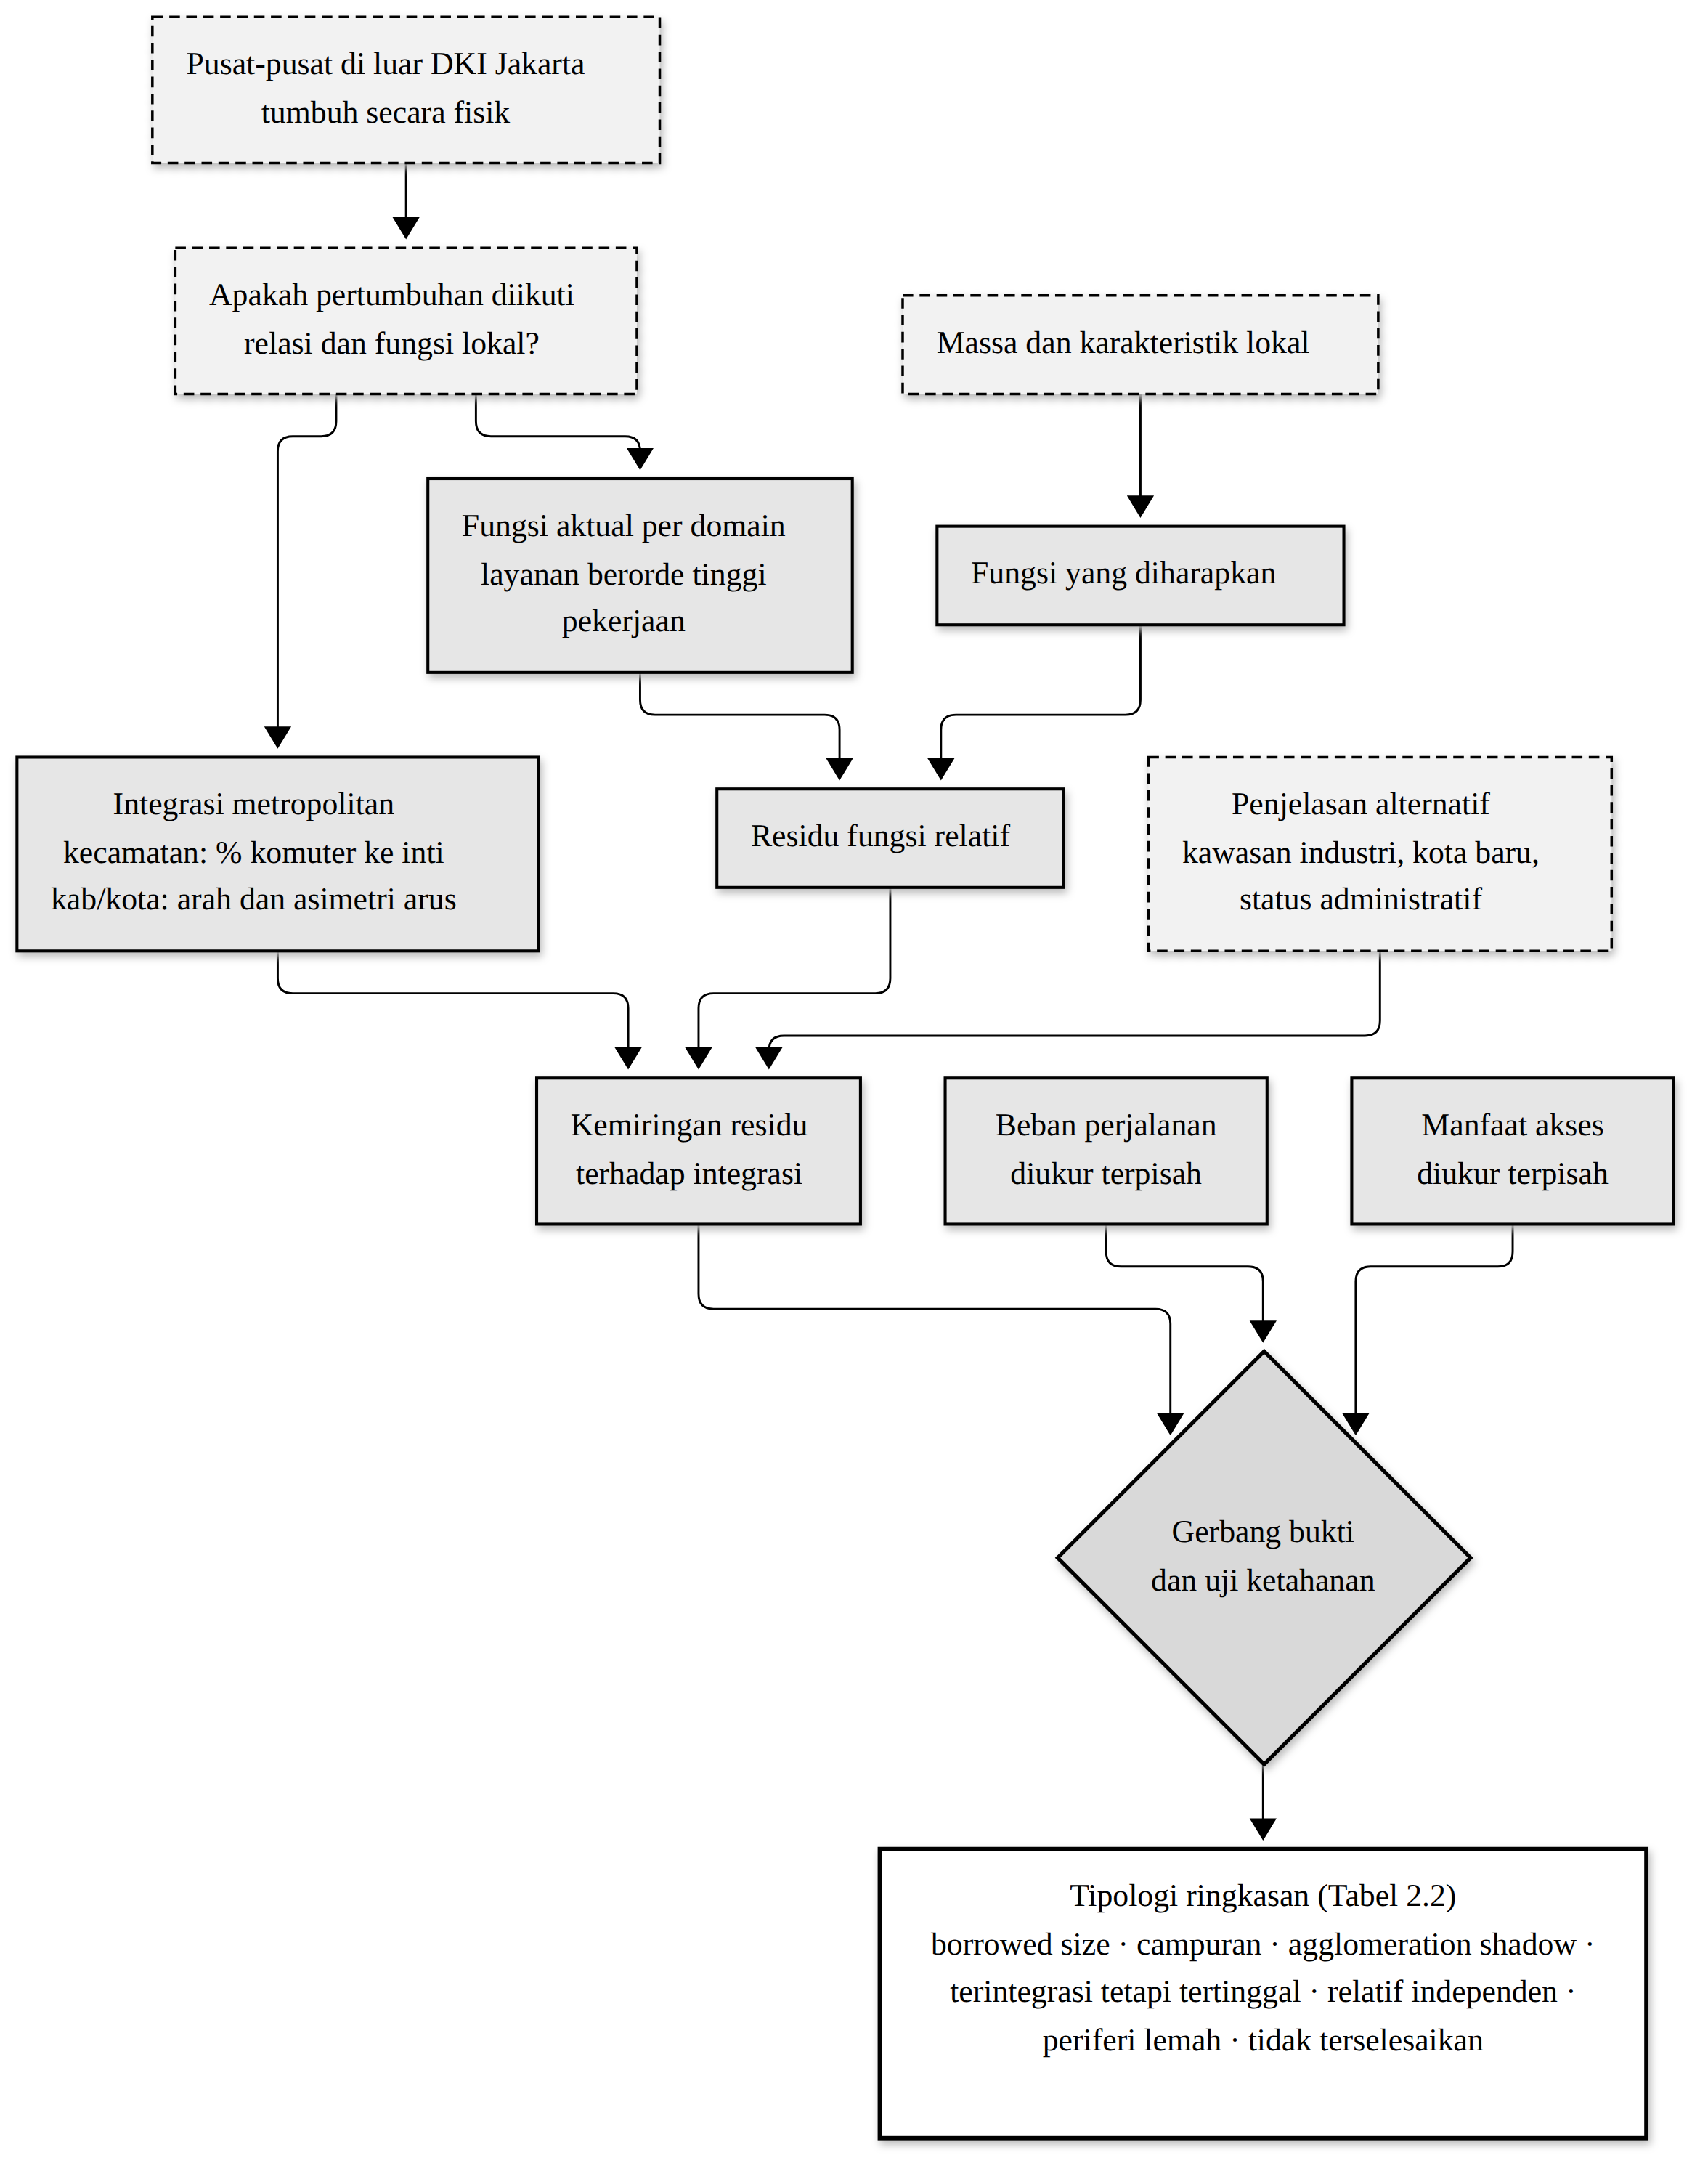
\includegraphics[width=0.72\textwidth]{figures/bab1_logika_penelitian.png}
  \caption{Logika masalah dan objek pengukuran penelitian. Relasi, fungsi relatif per domain, manfaat, dan beban diukur terpisah. Beban hanya dipakai pada gerbang label, dan kelas hasil mengikuti Tabel \ref{tab:tipologi}.}
  \label{fig:bab1-logika}
\end{figure}

\section{Rumusan masalah}

Transformasi metropolitan Jakarta telah membentuk pusat kegiatan di luar inti administratif. Keberadaan pusat tersebut belum menjelaskan kualitas relasinya dengan Jakarta ataupun kekuatan fungsi lokalnya. Hubungan metropolitan dapat berkaitan dengan surplus fungsi pada satu domain, defisit pada domain lain, manfaat akses, beban perjalanan, atau ketergantungan yang asimetris. Masalah penelitian terletak pada konfigurasi hubungan dan fungsi relatif yang teramati di wilayah Jabodetabek di luar DKI.

Masalah tersebut dirumuskan dalam tiga pertanyaan penelitian:

\begin{enumerate}
  \item Bagaimana arah, intensitas, dan asimetri relasi kabupaten/kota di luar DKI dengan Jakarta serta antarpinggiran, bagaimana relasi tersebut berubah pada 2014, 2019, dan 2023, dan bagaimana integrasi metropolitan tersebar antarkecamatan?
  \item Bagaimana fungsi relatif layanan dan pekerjaan setiap kecamatan dibandingkan dengan fungsi yang diharapkan dari massa lokalnya, serta bagaimana manfaat dan beban integrasi tersebar menurut kecamatan dan kabupaten/kota asal?
  \item Bagaimana integrasi metropolitan berhubungan dengan fungsi relatif setelah kondisi lokal dan penjelasan alternatif diperiksa, serta konfigurasi apa yang konsisten dengan \textit{borrowed size}, \textit{agglomeration shadow}, hasil campuran, atau hasil yang belum terselesaikan?
\end{enumerate}

Analisis sensitivitas tidak menjadi pertanyaan substantif tersendiri. Analisis tersebut dipakai untuk menilai ketahanan jawaban atas ketiga pertanyaan melalui perubahan garis dasar massa, pembanding, bentuk residu, komposisi indikator, dan ambang. Perubahan sumber yang mengubah konstruk dilaporkan sebagai triangulasi, bukan sebagai sensitivitas model yang ekuivalen.

\section{Tujuan penelitian}

Tujuan umum penelitian ini adalah menganalisis hubungan antara integrasi metropolitan dan fungsi relatif pusat-pusat sekunder Jabodetabek dengan membedakan domain fungsi, manfaat, beban, dan ketahanan hasil terhadap keputusan analitis.

Tujuan khusus penelitian adalah:

\begin{enumerate}
  \item Mengukur dan memetakan arah, intensitas, serta asimetri relasi kabupaten/kota di luar DKI dengan Jakarta dan antarpinggiran beserta perubahannya pada 2014, 2019, dan 2023, serta memetakan integrasi metropolitan per kecamatan.
  \item Mengukur fungsi relatif layanan dan pekerjaan per kecamatan terhadap fungsi yang diharapkan dari massa lokal, serta menyusun profil manfaat dan beban per kecamatan dan per kabupaten/kota asal.
  \item Menganalisis kemiringan hubungan integrasi dengan fungsi relatif setelah kondisi lokal dan penjelasan alternatif diperiksa, lalu mengidentifikasi konfigurasi yang konsisten dengan \textit{borrowed size}, \textit{agglomeration shadow}, hasil campuran, atau hasil yang belum terselesaikan.
\end{enumerate}

\section{Batasan penelitian}

Penelitian ini dibatasi pada Jabodetabek administratif yang mencakup DKI Jakarta, Kabupaten Bogor, Kota Bogor, Kota Depok, Kabupaten Tangerang, Kota Tangerang, Kota Tangerang Selatan, Kabupaten Bekasi, dan Kota Bekasi. Kabupaten Cianjur, yang termasuk Kawasan Aglomerasi, tidak dicakup. Cianjur berada pada lapisan luar sistem metropolitan dan tidak tercakup dalam Survei Komuter Jabodetabek. Pola yang ditemukan diduga juga relevan bagi Cianjur dengan intensitas yang lebih kecil, tetapi dugaan ini merupakan alasan pembatasan lingkup, bukan klaim empiris.

Tolok ukur fungsi dibentuk secara internal dari kecamatan di luar DKI; DKI Jakarta tidak dimasukkan ke dalam pembentukan ekspektasi karena kedudukannya sebagai inti. Karena residu terhadap tolok ukur internal berpusat di sekitar nol, tanda residu satu kecamatan bukan bukti \emph{shadow} atau \emph{borrowed size}. Bukti tersebut dibaca dari kemiringan hubungan residu terhadap integrasi.

Penelitian memakai dua tingkat unit. Tingkat utama adalah 141 kecamatan di luar DKI untuk mengukur integrasi, fungsi relatif, dan hubungan keduanya. Tingkat pendalaman adalah 13 kabupaten/kota (lima kota administrasi DKI dan delapan kabupaten/kota Bodetabek) untuk membaca relasi terarah, durasi, biaya, dan penghasilan komuter. Nilai kabupaten/kota tidak diturunkan ke kecamatan tanpa model eksplisit dan label estimasi. Pusat sekunder ditandai berdasarkan massa (penduduk dan volume terbangun hunian), bukan berdasarkan fungsi yang hendak diukur.

Penelitian bertumpu pada proksi dan sumber terbuka. Data pemerintah yang terbuka digunakan apabila sesuai, sedangkan data tertutup, permohonan kelembagaan, mikrodata berbayar, dan data ponsel individu bukan syarat rancangan. Setiap proksi dinilai berdasarkan kesesuaian konstruk, cakupan spasial dan temporal, keterulangan, biaya pemerolehan, lisensi, dan hasil pemeriksaan independen.

Analisis fungsi bersifat potong lintang dengan tahun rujukan 2024. Perubahan antarperiode hanya dianalisis pada relasi komuter 2014, 2019, dan 2023, karena tidak tersedia seri fungsi tingkat kecamatan yang sebanding.

Dua domain fungsi diperlakukan sama-sama utama. Domain layanan berorde tinggi diukur dari jumlah fasilitas per kecamatan dalam publikasi Statistik Potensi Desa 2024, dilengkapi direktori fasilitas. Domain pekerjaan diproksikan dengan volume terbangun nonhunian dari citra satelit. Istilah kematangan berarti kematangan fungsi lokal pada kedua domain tersebut, bukan kesejahteraan penduduk, mutu pelayanan secara menyeluruh, ketahanan ekonomi, atau keberhasilan pembangunan. Jumlah fasilitas tidak disebut produktivitas, dan volume nonhunian tidak disebut jumlah pekerjaan.

Rantai analisis minimum terdiri atas integrasi kecamatan, satu domain fungsi yang dibentuk secara independen, tolok ukur internal, dan kemiringan hubungan keduanya, ditambah profil relasi kabupaten/kota. Modul pengamatan lalu lintas dan media komunikasi interaktif dijelaskan pada Bab 3 sebagai penguatan.

Hasil penelitian bersifat observasional dan asosiasional. Penelitian ini tidak mengidentifikasi pengaruh kausal Jakarta terhadap pusat sekunder, tidak menetapkan satu radius metropolitan yang benar, dan tidak memprediksi dampak kebijakan. Istilah \emph{borrowed size} atau \emph{agglomeration shadow} digunakan sebagai interpretasi bersyarat setelah bukti relasional, fungsi relatif, penjelasan alternatif, dan ketahanan hasil diperiksa.

\section{Metode penelitian}

Penelitian ini memakai pendekatan kuantitatif dengan analisis spasial-relasional dalam desain studi kasus tunggal Jabodetabek. Tingkat kecamatan memakai persentase komuter menuju kawasan inti sebagai integrasi, jumlah fasilitas berorde tinggi dan volume terbangun nonhunian sebagai fungsi, serta penduduk sebagai massa. Fungsi harapan dibentuk dari kecamatan lain di luar DKI melalui prediksi \emph{leave-one-out}, lalu residu fungsi diregresikan terhadap integrasi dengan kontrol penjelasan alternatif. Tingkat kabupaten/kota memakai matriks asal-tujuan komuter 2014, 2019, dan 2023 untuk membaca arah, asimetri, dan perubahan relasi. Rincian sumber, operasionalisasi, dan langkah analisis disajikan pada Bab 3.

\section{Manfaat penelitian}

\subsection{Manfaat teoretis}

Secara teoretis, penelitian ini memperjelas penggunaan \emph{borrowed size} dan \emph{agglomeration shadow} dalam sistem metropolitan yang hierarkis dan didominasi satu inti. Penelitian memisahkan massa lokal dari fungsi aktual, kedekatan dari relasi yang terealisasi, serta kematangan fungsi lokal dari akses dan kesejahteraan. Pengujian terpisah untuk layanan dan pekerjaan memperlihatkan apakah kedua domain bergerak searah.

\subsection{Manfaat metodologis}

Secara metodologis, penelitian ini menyediakan alur yang dapat diaudit dari penandaan pusat berbasis massa sampai pengukuran relasi, tolok ukur fungsi, kemiringan hubungan per domain, manfaat dan beban, serta ketidakpastian hasil. Aturan satu indikator satu peran mengurangi hubungan matematis semu, dan seluruh sumber yang dipakai bersifat terbuka sehingga dapat diulang.

\subsection{Manfaat praktis}

Secara praktis, penelitian ini memberi gambaran terpilah tentang posisi kecamatan dan kabupaten/kota di sekitar Jakarta kepada pemerintah daerah, Dewan Kawasan Aglomerasi, dan penyusun rencana induk Kawasan Aglomerasi. Profil relasi, fungsi relatif, manfaat, dan beban dapat membedakan kebutuhan penguatan fungsi lokal, hubungan antarpusat, pengurangan beban perjalanan, dan koordinasi lintas batas. Penelitian juga dapat membuka arah perlakuan yang lebih baik bagi kawasan hunian berpenduduk besar yang layanannya tertinggal dari permintaan lokal. Keluaran ini bersifat diagnostik. Penelitian tidak menetapkan perubahan batas administrasi, memilih satu bentuk kelembagaan, atau memprediksi dampak kebijakan tanpa analisis tambahan.

\section{Struktur penulisan}

Penelitian ini disusun dalam enam bab. Bab 1 menjelaskan latar belakang, rumusan masalah, tujuan, batasan, ringkasan metode, manfaat, dan struktur penulisan. Bab 2 membangun konsep kunci, menyintesis penelitian terdahulu, dan menyusun kerangka konseptual yang menghubungkan massa lokal, relasi metropolitan, fungsi relatif, manfaat, beban, dan diagnosis bersyarat.

Bab 3 menjelaskan pendekatan dan desain dua tingkat, ruang lingkup, unit, sumber dan operasionalisasi variabel, serta langkah analisis. Bab 4 menggambarkan Jabodetabek sejauh diperlukan untuk memahami konteks kebijakan, demografi, struktur ekonomi, pola komuter, morfologi, jaringan, dan kawasan industri. Bab 5 menyajikan serta membahas hasil menurut pertanyaan penelitian. Bab 6 merangkum jawaban penelitian, batas inferensi, dan rekomendasi yang sesuai dengan temuan.

\clearpage

\chapter{Bab 2 Kajian Pustaka}

\section{Penjelasan konsep-konsep kunci}

Konsep dalam bab ini dipakai untuk membedakan objek yang sering tercampur dalam pembahasan metropolitan. Ukuran lokal, fungsi, kinerja, aksesibilitas, konektivitas, dan integrasi fungsional bukan sinonim. Sebuah pusat sekunder dapat mempunyai penduduk besar, akses yang baik, dan arus keluar yang kuat pada saat yang sama. Susunan seperti itu belum cukup untuk disebut peminjaman ukuran atau bayangan aglomerasi.

\subsection{Ekonomi aglomerasi dan disekonomi aglomerasi}

Ekonomi aglomerasi adalah manfaat yang muncul ketika rumah tangga dan perusahaan berdekatan dengan banyak orang, pekerja, pemasok, pengetahuan, infrastruktur, dan amenitas. Mekanisme yang sering digunakan untuk menjelaskannya ialah berbagi, mencocokkan, dan belajar: berbagi fasilitas atau input, mencocokkan kebutuhan perusahaan dengan tenaga kerja, serta memperoleh pembelajaran dan pengetahuan dari interaksi yang berulang \parencite{durantonpuga2004}. Konsentrasi juga menimbulkan biaya, seperti kemacetan, harga lahan, polusi, tekanan jaringan, dan kompetisi atas sumber daya. Karena manfaat dan biaya bergerak bersama dengan cara yang berbeda, aglomerasi tidak boleh diperlakukan sebagai keuntungan yang selalu positif.

Dalam penelitian ini, teori aglomerasi menjadi garis dasar untuk membaca hubungan ukuran dan fungsi. Jika pusat yang lebih besar cenderung menopang lebih banyak fungsi, maka fungsi pusat kecil yang melebihi ekspektasi ukurannya perlu dijelaskan melalui relasi lain, karakteristik khusus, atau kesalahan pengukuran. Kenaikan kepadatan juga tidak langsung berarti kenaikan produktivitas; arah hubungan dapat berubah menurut sektor, skala, kelompok sosial, dan kondisi wilayah.

\subsection{Ukuran lokal, fungsi metropolitan, dan kinerja}

Tiga objek dipisahkan sejak awal. Ukuran lokal adalah massa yang dimiliki unit, misalnya penduduk, tenaga kerja, jumlah usaha, luas terbangun, atau kepadatan. Fungsi metropolitan adalah kemampuan menyediakan kegiatan atau layanan yang melampaui kebutuhan rutin unit, seperti pekerjaan khusus, layanan kesehatan dan pendidikan berorde tinggi, layanan bisnis, fungsi budaya, atau pusat kegiatan. Kinerja adalah hasil yang dicapai, misalnya produktivitas, pendapatan, inovasi, atau kesejahteraan.

Satu pusat dapat besar secara demografis tetapi terbatas pada fungsi keputusan. Sebaliknya, pusat yang lebih kecil dapat mempunyai layanan yang lebih beragam daripada yang lazim bagi ukurannya. Jumlah fasilitas, pekerjaan, PDRB, dan kinerja kesejahteraan karena itu tidak boleh saling menggantikan tanpa penjelasan konstruk, satuan, dan batas interpretasi.

\subsection{Sistem perkotaan, hierarki pusat, dan pusat sekunder}

Sistem perkotaan merupakan himpunan pusat yang saling berhubungan melalui arus manusia, barang, jasa, modal, informasi, dan pembagian fungsi. Teori tempat sentral membantu menjelaskan mengapa layanan berorde tinggi memerlukan ambang permintaan dan jangkauan pasar yang lebih besar. Pandangan jaringan melengkapi penjelasan tersebut dengan menunjukkan bahwa fungsi sebuah pusat juga ditentukan oleh posisinya terhadap pusat lain dan oleh kualitas relasi di antara pusat-pusat tersebut \parencite{burgermeijers2016}.

Dalam penelitian ini, \textit{pusat sekunder} berarti konsentrasi massa di luar inti Jakarta yang berpotensi menjalankan fungsi subregional atau metropolitan. Status tersebut tidak ditentukan oleh label kota administratif, kedekatan dengan Jakarta, atau fungsi yang sudah menonjol. Penandaannya memakai massa saja, yaitu penduduk dan volume terbangun hunian, dengan ambang yang ditetapkan sebelum fungsi diukur. Memilih pusat dari fungsinya akan menyaring unit berdasarkan variabel hasil, sehingga tempat berpenduduk besar tetapi berfungsi sedikit, yang justru kandidat korban \textit{shadow}, tidak pernah masuk analisis.

\subsection{Polisentrisitas morfologis dan fungsional}

Polisentrisitas morfologis menunjuk pada keberadaan beberapa konsentrasi penduduk, pekerjaan, atau bangunan. Polisentrisitas fungsional menunjuk pada pola hubungan antarpusat, misalnya arus komuter, perjalanan, transaksi, atau jaringan organisasi. Hubungan antara kedua dimensi itu tidak otomatis kuat. Beberapa pusat dapat tampak seimbang pada peta, tetapi arusnya tetap terpusat pada Jakarta; sebaliknya, hubungan antarpusat dapat berkembang tanpa menghasilkan ukuran pusat yang seimbang \parencite{burgermeijers2012,degoeietal2010}.

Bukti Indonesia menunjukkan bahwa analisis morfologis dan fungsional dapat menghasilkan pembacaan yang berbeda. Karena itu, penelitian ini memetakan bentuk terbangun dan konsentrasi kegiatan sebagai satu lapisan, sedangkan arus dan hubungan sebagai lapisan lain \parencite{sadewoetal2021}. Istilah ``banyak pusat'' tidak digunakan sebagai sinonim pemerataan fungsi, kemandirian, atau keberhasilan integrasi.

\subsection{Aksesibilitas, konektivitas, dan integrasi fungsional}

Aksesibilitas adalah potensi menjangkau peluang dengan memperhitungkan lokasi peluang dan hambatan perjalanan. Konektivitas menunjukkan keberadaan dan kualitas hubungan dalam jaringan. Integrasi fungsional merujuk pada hubungan yang tampak melalui arus atau interaksi yang dapat diamati maupun diestimasi secara transparan. Jarak, waktu tempuh, atau jumlah simpul hanya memberi informasi tentang akses atau konektivitas potensial. Ketiganya belum membuktikan hubungan yang benar-benar digunakan.

Pembedaan ini mencegah waktu tempuh singkat dibaca sebagai integrasi aktual. Bukti integrasi yang lebih kuat dapat berasal dari pasangan asal dan tujuan komuter, perjalanan, transaksi, jaringan perusahaan, atau hubungan layanan. Bila bukti tersebut tidak tersedia, hasil akan disebut aksesibilitas potensial dan tidak diberi label hubungan fungsional secara berlebihan. Kajian Jakarta menunjukkan bahwa jaringan transportasi dapat mengubah struktur permukiman dan kegiatan, tetapi arah perubahan harus dipisahkan dari keberadaan infrastruktur itu sendiri \parencite{yudhistiraetal2019}.

\subsection{Kematangan fungsi lokal dan residu fungsi}

Kematangan fungsi lokal adalah posisi suatu pusat dalam menopang pekerjaan dan layanan yang dipilih sebagai domain penelitian, dibandingkan dengan pusat lain yang memiliki ukuran dan karakteristik lokal serupa. Istilah ini dibatasi pada keberadaan dan kapasitas fungsi yang terukur. Ia tidak menjadi ukuran langsung kesejahteraan, keterjangkauan layanan, mutu pelayanan secara menyeluruh, ketahanan ekonomi, atau keberhasilan pembangunan. Akses penduduk terhadap fungsi dan hasil yang mereka nikmati dilaporkan sebagai dimensi tersendiri.

Untuk fungsi $k$ pada unit $i$, fungsi yang diharapkan dapat ditulis sebagai:

\[
\widehat{F}_{ik}=f_k(S_i,X_i), \qquad R_{ik}=F_{ik}-\widehat{F}_{ik},
\]

\noindent dengan $F_{ik}$ sebagai fungsi yang diukur, $S_i$ sebagai ukuran lokal, $X_i$ sebagai karakteristik pembanding, dan $R_{ik}$ sebagai residu fungsi relatif. Dalam penelitian ini, ekspektasi dibentuk dari kecamatan Jabodetabek di luar DKI; DKI Jakarta tidak digunakan untuk membentuk garis ekspektasi, dan pembanding di luar Jabodetabek tidak dipakai. Residu positif berarti fungsi yang teramati lebih tinggi daripada pembanding internal tersebut, sedangkan residu negatif berarti lebih rendah. Karena tolok ukurnya internal, residu berpusat di sekitar nol menurut konstruksinya, dan kira-kira separuh unit pasti bertanda negatif. Tanda residu satu unit karena itu bukan bukti \textit{shadow}. \textit{Shadow} adalah defisit pada tingkat sistem; literatur rujukan membacanya dari koefisien hubungan antara kedekatan atau jaringan dan fungsi \parencite{burgeretal2015,meijersetal2016}. Penelitian ini membaca residu melalui kemiringan hubungannya dengan integrasi. Residu bukan bukti sebab atau ukuran universal kematangan kota.

\subsection{\textit{Borrowed size}}

\textit{Borrowed size} menjelaskan kemungkinan bahwa tempat yang lebih kecil memiliki fungsi atau kinerja yang biasanya diasosiasikan dengan kota yang lebih besar karena dapat mengakses manfaat aglomerasi melalui jaringan. Alonso memperkenalkan istilah ini untuk kota atau wilayah metropolitan kecil yang memperlihatkan sebagian karakteristik kota yang lebih besar karena berada dekat konsentrasi penduduk lain \parencite{alonso1973}. Rumusan berikutnya menyatakan bahwa peminjaman berlangsung melalui konektivitas dan fungsi yang dapat diidentifikasi, bukan melalui jarak semata \parencite{meijersburger2017,meijersetal2016,burgeretal2015}. Konsep ini menyangkut makna relatif: fungsi yang disandang suatu tempat dibandingkan dengan ukurannya, bukan skala absolut tempat tersebut.

Studi pada jaringan kota menunjukkan bahwa ukuran lokal, konektivitas, dan fungsi metropolitan dapat menghasilkan kombinasi yang tidak seragam. Bukti dari Tiongkok juga memperlihatkan bahwa kota kecil dapat memperoleh manfaat jaringan pada sebagian indikator, sedangkan hubungan dengan pusat besar pada indikator lain tetap bersifat kompetitif \parencite{yangzhudu2022,zhaomiaoxi2022}. Pendekatan tiga lapis yang lebih baru menambahkan kapasitas institusional dan relasional sebagai syarat agar manfaat akses dapat ditahan dan diubah menjadi fungsi lokal \parencite{otsuka2025}.

Dalam penelitian ini, pola baru disebut konsisten dengan \textit{borrowed size} hanya apabila terdapat bukti relasional yang memadai, surplus fungsi relatif terhadap ukuran lokal, kompatibilitas unit dan periode, serta ketahanan terhadap keputusan teknis. Jika satu syarat belum dipenuhi, istilah yang digunakan adalah surplus fungsi relatif atau akses metropolitan, bukan klaim mekanisme.

\subsection{\textit{Agglomeration shadow}}

\textit{Agglomeration shadow} adalah keadaan ketika kedekatan atau keterhubungan dengan pusat dominan berkaitan dengan fungsi lokal yang lebih rendah daripada yang sewajarnya diharapkan. Mekanismenya dapat melibatkan kompetisi atas permintaan, tenaga terampil, investasi, fungsi keputusan, atau layanan berorde tinggi. Konsep ini tidak menyatakan bahwa setiap pusat dekat Jakarta pasti dirugikan.

Kawasan hunian juga dapat menjadi korban \textit{shadow}. Penduduk yang besar menciptakan permintaan layanan lokal. Bila layanan berorde tinggi tetap defisit sementara orientasi penduduk ke inti tinggi, permintaan itu bocor ke inti, dan mekanisme ini lebih jelas menunjukkan \textit{shadow} daripada defisit pekerjaan. Pada domain pekerjaan, kawasan hunian yang memang direncanakan sebagai kota tidur dan kawasan hunian yang tertekan \textit{shadow} memberi sinyal yang sama, yaitu residu pekerjaan negatif dan arus keluar tinggi. Karena itu, klaim \textit{shadow} pada kawasan hunian memerlukan pembeda: domain layanan, atau perbandingan kawasan hunian bermassa serupa pada tingkat integrasi yang berbeda.

Bukti empiris memperlihatkan tanda yang berbeda menurut fungsi, skala, ukuran pusat, dan posisi jaringan. Integrasi regional dapat menyebarkan manufaktur sambil memusatkan jasa; jaringan kereta cepat dapat menghasilkan eksternalitas yang berbeda menurut sektor dan status administratif; dan kedekatan dengan kota besar pada beberapa kasus justru berkaitan dengan pertumbuhan pusat yang lebih kecil \parencite{zhenshilu2023,shietal2025,partridgeetal2009,sunding2016}. Karena itu, \textit{shadow} diperlakukan sebagai hasil pengujian relasional dan bukan sebagai asumsi yang diturunkan dari jarak.

\subsection{Spesialisasi fungsi, manfaat, dan ketergantungan asimetris}

Spesialisasi produksi tidak sama dengan kematangan fungsi. Fungsi produksi dapat menyebar ke pinggiran, sedangkan fungsi pengendalian, layanan bisnis, dan keputusan tetap terkonsentrasi di pusat besar \parencite{durantonpuga2005}. Penelitian Jakarta tentang kawasan industri dan Cikarang membantu menunjukkan dekonsentrasi pekerjaan dan keragaman asal pekerja, tetapi bukti tersebut belum dengan sendirinya membuktikan surplus fungsi metropolitan \parencite{hudalahetal2013,permatasarihudalah2013}.

Ketergantungan asimetris berarti hubungan penting bagi pusat sekunder, sementara kepentingan timbal baliknya tidak seimbang. Ia dapat tampak dalam dominasi tujuan komuter, ketergantungan pada layanan berorde tinggi di Jakarta, konsentrasi fungsi keputusan, atau beban infrastruktur yang tidak diimbangi kapasitas lokal. Manfaat akses dan ketergantungan dapat hadir bersamaan. Kajian akses pekerjaan di Jakarta menegaskan perlunya membedakan peluang yang tersedia, persaingan pencari kerja, penggunaan aktual, dan beban perjalanan \parencite{andani2021,aritenang2022,andani2025}.

\subsection{Kondisi campuran dan geografi fungsional}

Kategori campuran atau \textit{contested} digunakan ketika pusat menikmati surplus pada satu fungsi tetapi defisit pada fungsi lain, atau memperoleh manfaat sekaligus menanggung beban yang tinggi. Kategori ini menggambarkan perbedaan substantif antardomain. Perubahan kelas akibat indikator, ambang, atau unit ditempatkan sebagai ketidakstabilan hasil dan dilaporkan sebagai belum terselesaikan. Istilah \textit{transisional} hanya digunakan apabila perubahan antarperiode yang sebanding benar-benar diamati.

Geografi fungsional dibentuk oleh arus, waktu tempuh, wilayah tangkapan, dan jangkauan pasar; yurisdiksi administratif menentukan kewenangan, pelayanan, dan akuntabilitas. Penelitian dapat memetakan hubungan yang melintasi batas, tetapi jejak fungsional tersebut tidak boleh dibaca sebagai perluasan wilayah administratif Jakarta. Kerangka wilayah urban fungsional dapat menjadi rujukan, tetapi definisi dan unitnya harus diadaptasi secara terbuka terhadap data Indonesia.

\subsection{Diagnosis, sensitivitas, dan skenario}

Diagnosis \textit{status quo} menggunakan observasi untuk menggambarkan relasi, fungsi relatif, manfaat, dan beban. Analisis sensitivitas mengubah indikator, bobot, ambang, unit, atau spesifikasi yang masih mengestimasi objek sejenis. Skenario mengubah nilai atau asumsi secara eksplisit untuk membaca konsekuensi kondisional; skenario bukan ramalan dan bukan bukti perubahan kausal. Dengan pembedaan ini, perubahan kelas akibat pergantian sumber tidak disamakan dengan perubahan fenomena.

\section{Kajian penelitian terdahulu}

Subbab ini membahas penelitian empiris tentang Jakarta dan Jabodetabek. Sumber konseptual serta pembanding internasional ditempatkan pada Subbab 2.1 dan 2.3 untuk membangun teori, mekanisme, dan batas interpretasi. Di sini, penelitian terdahulu disusun sebagai rangkaian pengetahuan tentang perubahan pinggiran Jakarta, cara pengetahuan itu diperoleh, dan persoalan yang masih terbuka.

\subsection{Dari dormitori menuju pusat kegiatan pinggiran}

Penelitian Jakarta mula-mula menunjukkan kuatnya ketergantungan kota baru dan permukiman pinggiran terhadap inti. Kajian berikutnya mencatat pergeseran sebagian kawasan menuju susunan yang lebih beragam melalui kota baru, kawasan industri, pusat perdagangan, dan layanan yang dikelola swasta. Perubahan tersebut tidak berlangsung merata dan tetap disertai fragmentasi tata kelola, segregasi, serta hubungan komuter dengan Jakarta \parencite{hudalahfirman2012,firmanfahmi2017}.

Dekonsentrasi manufaktur memberi bukti paling nyata tentang perpindahan kegiatan ekonomi. Kawasan industri di pinggiran menangkap pertumbuhan pekerjaan dan membentuk spesialisasi baru. Studi pekerja Cikarang juga menemukan perjalanan lokal, perjalanan dari kota perluasan, dan perjalanan antarpinggiran menuju pusat pekerjaan tersebut \parencite{hudalahetal2013,permatasarihudalah2013}. Namun, keberadaan pekerjaan manufaktur belum menunjukkan bahwa fungsi keputusan, layanan bisnis, atau manfaat ekonomi telah tertahan di lokasi yang sama.

\subsection{Bentuk perkotaan, jaringan, dan perubahan aktivitas}

Jaringan jalan dan rel berhubungan dengan perubahan kepadatan penduduk, cahaya malam, perluasan lahan terbangun, dan penyebaran kegiatan. Yudhistira dan kolega menunjukkan bahwa pengaruh tersebut berbeda menurut moda dan jenis pinggiran. Pratama dan kolega menemukan bahwa peningkatan akses jalan tol berkaitan dengan perkembangan terbangun yang lebih menyebar pada bagian tertentu kawasan metropolitan \parencite{yudhistiraetal2019,pratamaetal2022}. Kedua penelitian itu menjelaskan perubahan struktur, tetapi tidak menjadikan akses jaringan sebagai bukti langsung integrasi yang terealisasi atau kematangan fungsi lokal.

Perbedaan antara bentuk dan hubungan juga terlihat pada kajian polisentrisitas Indonesia. Pusat yang tampak kuat dari konsentrasi penduduk atau pekerjaan belum tentu mempunyai arus yang seimbang dengan pusat lain \parencite{sadewoetal2021}. Karena itu, penelitian ini menempatkan morfologi, aksesibilitas, dan relasi aktual sebagai tiga lapisan pengukuran yang berbeda.

\subsection{Komuter, akses pekerjaan, manfaat, dan beban}

Kajian komuter memperlihatkan struktur metropolitan yang campuran. Arus antarpinggiran menunjukkan tumbuhnya pusat kegiatan di luar Jakarta, sedangkan arus pinggiran ke inti tetap besar. Perbedaan pendapatan, tempat tinggal, moda, durasi, dan arah perjalanan juga membuat manfaat integrasi tidak terbagi secara merata \parencite{aritenang2023,aritenang2022}. Angkutan berbasis sepeda motor merupakan bagian lain dari hubungan metropolitan tersebut \parencite{aritenang2024}.

Penelitian akses pekerjaan menunjukkan perbedaan lain antara peluang potensial dan penggunaan aktual. Perhitungan akses menurut moda menemukan pemusatan peluang di bagian inti dan ketimpangan yang tinggi pada angkutan umum. Evaluasi koridor tol menunjukkan bahwa penurunan waktu tempuh dapat disertai kenaikan persaingan antarpencari kerja \parencite{andani2025,andani2021}. Temuan tersebut menjadi dasar untuk melaporkan manfaat dan beban secara terpisah, bukan meleburkannya menjadi satu skor bersih.

\subsection{Celah dan posisi penelitian}

Penelitian Jakarta telah menjelaskan transformasi pinggiran, dekonsentrasi manufaktur, perubahan bentuk terbangun, komuter, akses pekerjaan, dan ketimpangan mobilitas. Korpus yang ditelusuri belum menggabungkan relasi metropolitan terarah dengan fungsi relatif per domain, distribusi manfaat dan beban, serta ketahanan klasifikasi pada pusat-pusat sekunder Jabodetabek. Celah ini dibatasi pada sumber yang ditelusuri dan tidak digunakan untuk mengklaim bahwa tidak ada penelitian lain di luar korpus.

Penelitian ini meneruskan estafet tersebut dengan tiga langkah. Pertama, relasi dengan Jakarta dan pusat lain diukur menurut arah, intensitas, serta asimetri. Kedua, fungsi yang diamati atau diestimasi dibandingkan dengan nilai yang diharapkan menurut massa dan karakteristik lokal. Ketiga, diagnosis diuji terhadap perbedaan domain, unit, indikator, dan spesifikasi. Kebaruannya terletak pada perangkaian ketiga langkah tersebut untuk membedakan pola yang konsisten dengan \textit{borrowed size}, \textit{agglomeration shadow}, hasil campuran, atau hasil yang belum terselesaikan.

\clearpage
\begin{landscape}
\scriptsize
\setlength{\tabcolsep}{2.2pt}
\renewcommand{\arraystretch}{1.18}
\begin{longtable}{>{\centering\arraybackslash}p{0.55cm}p{3.4cm}p{3.0cm}p{3.6cm}p{3.9cm}p{4.0cm}p{4.5cm}}
\caption{Penelitian terdahulu terkait Jakarta dan Jabodetabek}\label{tab:penelitian-terdahulu}\\
\toprule
\textbf{No.} & \textbf{Judul Penelitian} & \textbf{Nama Peneliti} & \textbf{Tujuan Penelitian} & \textbf{Metode, Data, dan Unit Analisis} & \textbf{Hasil Penelitian} & \textbf{Celah dan Posisi Penelitian Ini}\\
\midrule
\endfirsthead
\multicolumn{7}{l}{\textit{Lanjutan Tabel \thetable}}\\
\toprule
\textbf{No.} & \textbf{Judul Penelitian} & \textbf{Nama Peneliti} & \textbf{Tujuan Penelitian} & \textbf{Metode, Data, dan Unit Analisis} & \textbf{Hasil Penelitian} & \textbf{Celah dan Posisi Penelitian Ini}\\
\midrule
\endhead
\midrule
\multicolumn{7}{r}{\textit{Bersambung ke halaman berikutnya}}\\
\endfoot
\bottomrule
\endlastfoot
1 & \textit{Identifying Post-suburbanization: The Case of the Jakarta Metropolitan Area (JMA)} & Adiwan F. Aritenang (2023) & Memeriksa kemandirian spasial, kematangan pinggiran, dan segregasi dalam proses pascasuburbanisasi. & Analisis deskriptif dan spasial Survei Komuter BPS 2014 dan 2019; arus antardistrik dan karakter sosial ekonomi komuter. & Arus antarpinggiran menunjukkan pusat kegiatan baru, tetapi arus menuju inti tetap kuat. Kematangan pinggiran berjalan bersama segregasi. & Belum membandingkan fungsi yang diamati dengan fungsi yang diharapkan menurut ukuran pusat. Penelitian ini memasangkan arus dengan fungsi relatif dan stabilitas diagnosis.\\
2 & \textit{Pola Pergerakan dan Dekonsentrasi Pekerjaan di Kawasan Metropolitan: Studi Kasus Pekerja Industri Cikarang, Bekasi} & Putri Sugih Permatasari dan Delik Hudalah (2013) & Mengidentifikasi pola perjalanan pekerja industri Cikarang dan karakteristik yang berkaitan dengannya. & Kuesioner terhadap 116 pekerja; statistik deskriptif, pemetaan asal tempat tinggal, uji Chi-Square, dan Cramer. & Cikarang menarik pekerja lokal serta pekerja dari kota perluasan dan pinggiran lain, yang menunjukkan keberadaan pusat pekerjaan di luar inti. & Sampel purposif dan satu sektor tidak mewakili arus Jabodetabek. Penelitian ini membandingkan beberapa pusat, arah relasi, fungsi, manfaat, dan beban.\\
3 & \textit{Industrial Land Development and Manufacturing Deconcentration in Greater Jakarta} & Delik Hudalah, Dimitra Viantari, Tommy Firman, dan Johan Woltjer (2013) & Menilai dekonsentrasi manufaktur dan pengaruhnya terhadap struktur spasial Greater Jakarta. & Pemetaan rasio pekerjaan dan penduduk pada 1995, 2001, dan 2010; data kawasan industri dan \textit{location quotient}. & Pertumbuhan bersih manufaktur terkonsentrasi di pinggiran luar dan pusat industri terencana serta membentuk spesialisasi sektoral. & Dekonsentrasi pekerjaan belum membuktikan perpindahan fungsi keputusan atau retensi manfaat. Penelitian ini menilai fungsi relatif lintasdomain dan relasinya.\\
4 & \textit{Beyond Property: Industrial Estates and Post-suburban Transformation in Jakarta Metropolitan Region} & Delik Hudalah dan Tommy Firman (2012) & Menjelaskan peran kawasan industri dan pengembang swasta dalam transformasi pascasuburban Jakarta. & Kajian transformasi kawasan industri dan peran aktor pada pinggiran metropolitan. & Kawasan industri memperbesar peran ekonomi pinggiran dan mendorong perubahan dari kawasan hunian menuju pusat kegiatan yang lebih beragam. & Tidak menyediakan diagnosis komparatif antarpusat atau tolok ukur fungsi relatif. Penelitian ini menguji variasi pusat secara kuantitatif.\\
5 & \textit{The Privatization of Metropolitan Jakarta's (Jabodetabek) Urban Fringes: The Early Stages of Post-Suburbanization in Indonesia} & Tommy Firman dan Fikri Zul Fahmi (2017) & Menilai apakah perubahan pinggiran Jabodetabek menunjukkan tahap awal pascasuburbanisasi dan bagaimana privatisasi membentuknya. & Analisis deskriptif perubahan fisik, kota baru, kawasan industri, dan hubungan pemerintah dengan pengembang swasta. & Sebagian pinggiran memperoleh pekerjaan dan layanan baru, tetapi perkembangannya tetap terfragmentasi dan hubungan dengan inti masih kuat. & Kematangan dibahas secara deskriptif. Penelitian ini mengukurnya melalui relasi, fungsi relatif, manfaat, dan beban per pusat.\\
6 & \textit{Transportation Network and Changes in Urban Structure: Evidence from the Jakarta Metropolitan Area} & Muhammad Halley Yudhistira, Witri Indriyani, Andhika Putra Pratama, Yusuf Sofiyandi, dan Yusuf Reza Kurniawan (2019) & Menguji hubungan akses jalan dan rel dengan perubahan kepadatan penduduk serta aktivitas perkotaan. & Data 1.483 komunitas, sensus 2000 dan 2010, cahaya malam, akses jaringan, dan variabel instrumental. & Jalan dan rel berkaitan dengan suburbanisasi, tetapi besar serta arahnya berbeda menurut moda, zona, dan indikator. & Akses jaringan belum menunjukkan arus aktual atau kematangan fungsi. Penelitian ini memisahkan aksesibilitas dari integrasi yang terealisasi.\\
7 & \textit{Highway Expansion and Urban Sprawl in the Jakarta Metropolitan Area} & Andhika Putra Pratama, Muhammad Halley Yudhistira, dan Eric Koomen (2022) & Menguji hubungan perluasan jalan tol dengan ekspansi lahan terbangun dan penyebaran pembangunan. & Perubahan lahan terbangun 1990 sampai 2014 dan strategi variabel instrumental dengan jaringan historis. & Peningkatan akses tol berkaitan dengan pembangunan yang lebih menyebar, terutama pada radius sekitar 40 sampai 50 km dari pusat Jakarta. & Perluasan fisik tidak sama dengan pusat yang matang. Penelitian ini menempatkan morfologi sebagai konteks bagi fungsi dan relasi.\\
8 & \textit{Examining Socio-Economic Inequality Among Commuters: The Case of the Jakarta Metropolitan Area} & Adiwan Aritenang (2022) & Memeriksa perbedaan moda, arah perjalanan, durasi, dan kondisi kesehatan komuter menurut pendapatan. & Sekitar 13.000 pengamatan Survei Komuter BPS 2019; statistik deskriptif, uji nonparametrik, dan regresi logistik. & Komuter pinggiran berpendapatan tinggi lebih banyak menuju inti, sedangkan kelompok berpendapatan rendah lebih banyak bergerak antarpinggiran dan menanggung beban perjalanan tertentu. & Analisis individu belum dihubungkan dengan fungsi relatif pusat. Penelitian ini menempatkan beban pada kelompok dan lokasi yang sesuai tanpa menghapus heterogenitas.\\
9 & \textit{The Crucial Role of Motorcycle-Based Ride-Hailing Among Commuters: The Case of Jakarta and Bandung Metropolitan Areas} & Adiwan Fahlan Aritenang (2024) & Menilai penggunaan angkutan berbasis sepeda motor dan karakter sosial, ekonomi, serta spasial penggunanya. & Survei rumah tangga komuter JMA 2019 dan BMA 2017; statistik deskriptif serta regresi logistik. & Pengguna terutama berasal dari kelompok muda dan berpendapatan lebih rendah; moda ini mendukung mobilitas antarpinggiran. & Belum mengukur fungsi pusat atau hubungan antarpusat secara lengkap. Penelitian ini memakai temuan tersebut untuk menjaga pembacaan integrasi tetap multimoda.\\
10 & \textit{Spatial, Mobility, or Socio-economic Inequity? A District-Level Job Accessibility Evaluation in Jakarta, Indonesia} & I Gusti Ayu Andani, Nadia Qamilla, Rakan Pramoe Izdihar, Maya Safira, Anjar Dimara Sakti, dan Ibnu Syabri (2025) & Mengevaluasi ketimpangan akses pekerjaan menurut lokasi, pendapatan, dan moda. & TAZ Jakarta, waktu perjalanan Google Maps, OD hasil model, akses kumulatif, Gini, Palma, dan Theil. & Akses pekerjaan terpusat di inti. Angkutan umum memiliki distribusi paling timpang, sedangkan sepeda motor memberi jangkauan lebih merata. & Wilayah kajian terutama Jakarta dan aksesnya bersifat potensial. Penelitian ini memperluas cakupan ke pusat sekunder Jabodetabek serta memisahkan akses dari arus aktual.\\
11 & \textit{Job Access and Spatial Equity of a Toll Road} & I Gusti Ayu Andani, Lissy C. La Paix Puello, Shanty Yulianti Rachmat, Ibnu Syabri, dan Karst Geurs (2021) & Mengevaluasi dampak Jalan Tol Cipularang terhadap akses pekerjaan dan keadilan spasial. & Model transportasi 229 distrik; skenario dengan dan tanpa tol, akses potensial, indeks Shen, Gini, Palma, dan klaster. & Tol menurunkan waktu tempuh, tetapi persaingan antarpencari kerja dapat mengurangi jumlah pekerjaan yang dapat diakses per pekerja. & Koridor kajian melampaui Jabodetabek dan hasilnya berbasis simulasi. Penelitian ini mengambil logika pemisahan akses, kompetisi, dan distribusi manfaat.\\
12 & \textit{Using Morphological and Functional Polycentricity Analyses to Study the Indonesian Urban Spatial Structure: The Case of Medan, Jakarta, and Denpasar} & Erie Sadewo, Ibnu Syabri, Anzhelika Antipova, Pradono, dan Delik Hudalah (2021) & Mengidentifikasi subpusat dan membandingkan polisentrisitas morfologis serta fungsional di tiga metropolitan Indonesia. & Identifikasi subpusat dari sensus ekonomi terbaru dan analisis arus dari survei komuter; perbandingan Medan, Jakarta, dan Denpasar. & Metropolitan Jakarta berstruktur polisentris, sedangkan Medan dan Denpasar monosentris. Perbedaannya dikaitkan dengan lintasan industrialisasi, bukan strategi tata ruang. & Polisentrisitas diukur pada tingkat struktur, belum sebagai fungsi relatif tiap pusat terhadap massanya. Penelitian ini membandingkan fungsi aktual dengan harapan dari massa.\\
13 & \textit{The Role of Urban Transformation on Inter-Suburban Commuting: Evidence from Jakarta Metropolitan Area, Indonesia} & Erie Sadewo, Delik Hudalah, Anzhelika Antipova, Long Cheng, dan Ibnu Syabri (2023) & Menguji pengaruh desentralisasi pekerjaan dan amenitas pinggiran terhadap dinamika komuter antarpinggiran. & Regresi panel spasial komuter antarpinggiran tingkat kabupaten/kota, 2008--2015, dari data komuter Sakernas. & Ekspansi pekerjaan pinggiran akibat desentralisasi industri diikuti kenaikan komuter antarpinggiran. Subpusat industri monofungsi menarik komuter dari pinggiran lain, tetapi juga mendorong penduduk mencari kerja jasa di tempat lain. & Preseden terdekat bagi relasi antarpinggiran. Belum menghubungkan relasi dengan fungsi relatif per domain atau memisahkan manfaat dari beban. Penelitian ini menguji kemiringan fungsi relatif terhadap integrasi.\\
\end{longtable}
\end{landscape}
\clearpage

\section{Kerangka teori dan kerangka konseptual}

\subsection{Rantai mekanisme}

Kerangka penelitian menghubungkan empat lapisan. Lapisan pertama adalah massa dan biaya lokal: ukuran, kepadatan, struktur ekonomi, lahan, dan infrastruktur membentuk kapasitas dasar sekaligus tekanan. Lapisan kedua adalah eksternalitas jaringan: hubungan dengan Jakarta dan pusat lain membuka akses ke pasar, pekerja, pengetahuan, dan layanan di luar kapasitas lokal. Lapisan ketiga adalah pembagian fungsi dan polarisasi: jaringan dapat menyebarkan produksi, tetapi tetap memusatkan fungsi keputusan, layanan strategis, atau permintaan tertentu. Lapisan keempat adalah kondisi perantara: hierarki, spesialisasi, status administratif, modal kelembagaan, dan posisi jaringan memengaruhi apakah manfaat dapat ditahan di pusat sekunder.

Rantai tersebut tidak diasumsikan berjalan satu arah. Pusat yang sama dapat meminjam layanan tertentu, bergantung pada Jakarta untuk fungsi lain, dan menanggung beban perjalanan pada dimensi ketiga. Kerangka ini menjelaskan mengapa kategori campuran dipertahankan dan mengapa hasil dianalisis per domain sebelum diringkas.

\begin{figure}[H]
  \centering
  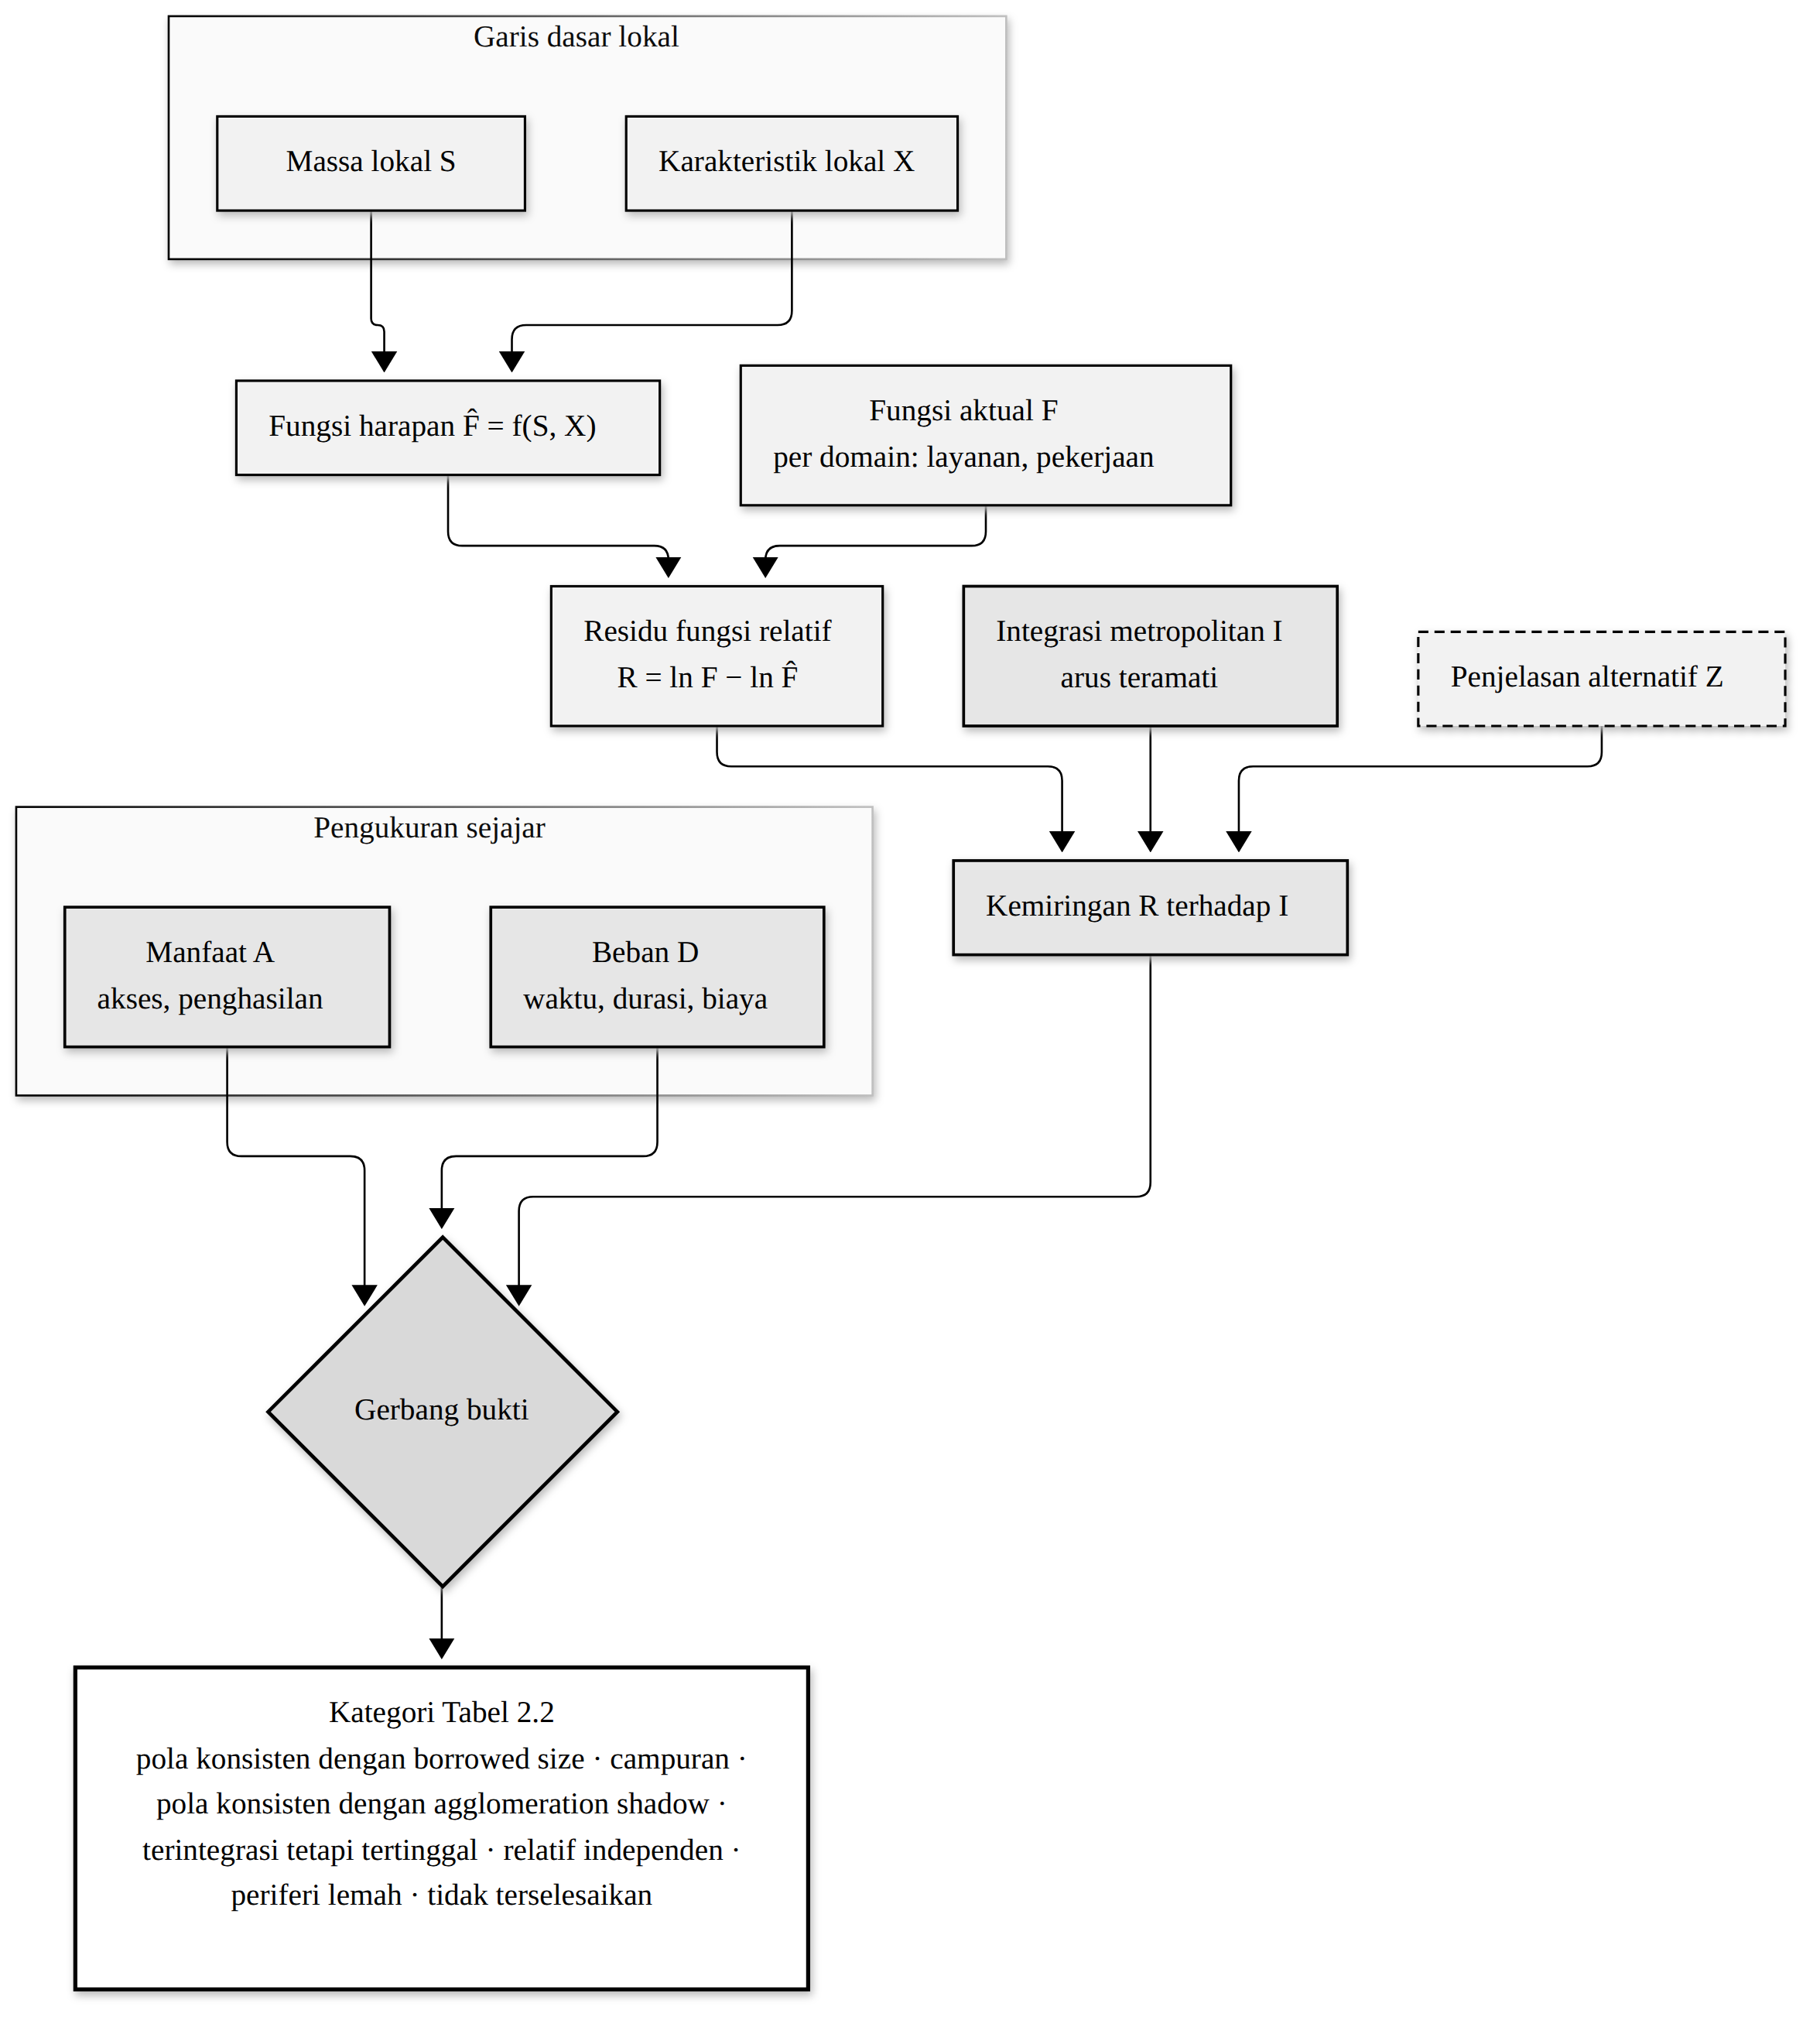
\includegraphics[width=0.74\textwidth]{figures/bab2_kerangka_konseptual.png}
  \caption{Kerangka konseptual. Massa $S$ dan karakteristik lokal $X$ membentuk fungsi harapan $\widehat F$; residu $R$ diuji terhadap integrasi $I$ dengan kontrol penjelasan alternatif $Z$. Manfaat dan beban diukur sejajar dan terpisah. Nama hasil mengikuti Tabel \ref{tab:tipologi}. Panah menunjukkan urutan pengukuran, bukan hubungan kausal yang telah terbukti.}
  \label{fig:bab2-kerangka-konseptual}
\end{figure}

\subsection{Model pengukuran konseptual}

Untuk setiap pusat $i$ dan domain fungsi $k$, penelitian membedakan:

\begin{enumerate}
  \item Ukuran dan karakteristik lokal $(S_i,X_i)$;
  \item Integrasi relasional $(I_i)$ yang idealnya berasal dari arus atau interaksi;
  \item Fungsi aktual $(F_{ik})$;
  \item Fungsi yang diharapkan $(\widehat{F}_{ik})$;
  \item Residu fungsi relatif $(R_{ik})$;
  \item Manfaat akses $(A_{ik})$;
  \item Beban atau ketergantungan $(D_{ik})$; dan
  \item Ketahanan klasifikasi $(Q_i)$ berdasarkan variasi spesifikasi yang masih masuk akal.
\end{enumerate}

Hubungan konseptualnya dapat ditulis sebagai:

\[
R_{ik}=g_k(I_i,S_i,X_i,Z_i)+\varepsilon_{ik},
\]

\noindent dengan $Z_i$ sebagai penjelasan alternatif. Karena $S_i$ dan $X_i$ sudah dipakai untuk membentuk $\widehat F_{ik}$, hubungan yang diuji pada Bab 3 adalah kemiringan $R_{ik}$ terhadap $I_i$ setelah $Z_i$ dikontrol. Kemiringan inilah yang membedakan \textit{borrowed size} dari \textit{shadow}, bukan tanda residu per unit. Persamaan ini bukan komitmen pada model kausal. Ia menunjukkan objek yang dipisahkan: fungsi relatif sebagai keluaran, ukuran dan karakteristik lokal sebagai garis dasar, integrasi sebagai relasi, manfaat dan beban sebagai pengukuran sejajar, serta penjelasan alternatif dan ketidakpastian sebagai pemeriksaan.

\subsection{Tipologi diagnosis sementara}

Tipologi berikut menjadi ringkasan akhir setelah inferensi kemiringan dan gerbang bukti. Daftar tujuh kategori ini dipakai seragam pada Bab 1, Bab 2, dan Bab 3. Integrasi disebut tinggi atau rendah terhadap ambang yang dibekukan sebelum klasifikasi. Residu disebut positif atau negatif hanya bila selang ketidakpastiannya tidak memuat nol. Beban diukur terpisah dari integrasi maupun residu.

\begin{table}[H]
\centering
\caption{Tipologi diagnosis berdasarkan integrasi, residu fungsi, dan beban}
\label{tab:tipologi}
\begin{adjustbox}{max width=\textwidth}
\begin{tabular}{>{\raggedright\arraybackslash}p{0.10\textwidth}>{\raggedright\arraybackslash}p{0.20\textwidth}>{\raggedright\arraybackslash}p{0.17\textwidth}>{\raggedright\arraybackslash}p{0.20\textwidth}>{\raggedright\arraybackslash}p{0.29\textwidth}}
\toprule
\textbf{Integrasi} & \textbf{Residu} & \textbf{Beban} & \textbf{Kategori} & \textbf{Interpretasi aman}\\
\midrule
Tinggi & Positif & Rendah hingga sedang & Pola konsisten dengan \textit{borrowed size} & Akses jaringan berasosiasi dengan fungsi relatif yang lebih besar.\\
Tinggi & Positif pada satu domain, negatif pada domain lain; atau positif dengan beban tinggi & Bervariasi & Campuran atau \textit{contested} & Surplus hadir bersama defisit pada domain lain atau bersama beban yang tinggi.\\
Tinggi & Negatif & Tinggi, diukur terpisah dari integrasi dan residu & Pola konsisten dengan \textit{agglomeration shadow} & Integrasi disertai defisit fungsi dan beban yang independen; tidak membuktikan bahwa Jakarta menyebabkan defisit.\\
Tinggi & Negatif & Rendah atau belum terbukti & Terintegrasi tetapi tertinggal & Belum cukup bukti untuk label \textit{shadow}.\\
Rendah & Positif & Bervariasi & Relatif independen & Surplus tidak terutama dibaca sebagai hasil hubungan dengan Jakarta; bukan bukti autarki.\\
Rendah & Negatif & Bervariasi & Periferi lemah & Basis lokal dan hubungan metropolitan sama-sama terbatas; tidak disebut \textit{shadow}.\\
\multicolumn{3}{>{\raggedright\arraybackslash}p{0.50\textwidth}}{Komponen wajib hilang, selang residu memuat nol, atau kelas berubah pada spesifikasi utama} & Tidak terselesaikan & Ketidakpastian dilaporkan sebagai hasil, bukan dipaksa ke kelas terdekat.\\
\bottomrule
\end{tabular}
\end{adjustbox}
\end{table}

Kelas tidak dihitung kembali sebagai indikator beban, dan indeks komposit tidak dipakai bila menyembunyikan perbedaan domain. Karena residu dibentuk secara internal, banyaknya unit pada kelas tertentu bukan bukti \textit{shadow} atau \textit{borrowed size} pada tingkat sistem. Bukti tersebut dibaca dari kemiringan pada Bab 3.

\subsection{Proposisi empiris}

Proposisi berikut berarah dan masing-masing memiliki hasil yang dapat membantahnya. Proposisi ini menjadi panduan pengujian, bukan hipotesis kausal.

\begin{table}[H]
\centering
\footnotesize
\caption{Proposisi empiris dan hasil yang membantahnya}
\label{tab:proposisi}
\begin{tabularx}{\textwidth}{>{\raggedright\arraybackslash}p{0.12\textwidth} >{\raggedright\arraybackslash}X >{\raggedright\arraybackslash}p{0.27\textwidth}}
\toprule
\textbf{Kode} & \textbf{Proposisi} & \textbf{Hasil yang membantah}\\
\midrule
P1 (layanan, kecamatan) & Setelah massa dan karakteristik lokal diperhitungkan, integrasi yang lebih tinggi berasosiasi dengan residu layanan berorde tinggi yang lebih rendah. Pola ini diharapkan paling jelas pada kecamatan berpenduduk besar yang dominan hunian. & Kemiringan nol atau positif yang stabil.\\
P2 (pekerjaan, koridor industri) & Kabupaten/kota dengan tarikan masuk dan arus antarpinggiran yang besar, serta kecamatan di koridor industri Bekasi--Cikarang dan Tangerang, memiliki residu pekerjaan positif, sehingga konsisten dengan \textit{borrowed size} pada domain produksi. & Residu pekerjaan negatif pada unit dengan tarikan masuk tertinggi.\\
P3 (lintas domain) & Unit yang sama dapat surplus pekerjaan tetapi defisit layanan, sejalan dengan spesialisasi fungsional \parencite{durantonpuga2005}, sehingga masuk kategori campuran. & Tanda residu kedua domain selalu searah.\\
P4 (gradien, opsional) & Hubungan integrasi--residu tidak linear sepanjang gradien integrasi. & Tidak ada perubahan kemiringan pada spesifikasi yang wajar.\\
\bottomrule
\end{tabularx}
\end{table}

\subsection{Gerbang penggunaan label}

Label \textit{borrowed size} atau \textit{agglomeration shadow} digunakan hanya jika empat syarat terpenuhi:

\begin{enumerate}
  \item Terdapat bukti relasional teramati, bukan hanya jarak atau waktu tempuh;
  \item Fungsi aktual dibandingkan dengan ekspektasi ukuran pada unit pembanding yang memadai;
  \item Unit, periode, populasi sasaran, dan konstruk cukup kompatibel; dan
  \item Arah hubungan tidak bergantung pada satu proksi lemah atau satu keputusan teknis.
\end{enumerate}

Khusus label \textit{agglomeration shadow}, defisit fungsi harus disertai beban yang diukur terpisah dari residu \emph{dan} dari integrasi. Orientasi atau ketidakseimbangan arus tidak dipakai sebagai beban, karena indikator yang sama sudah membentuk integrasi. Beban diambil dari durasi, jarak, waktu tempuh, atau biaya perjalanan. Tanpa bukti tersebut, hasil disebut terintegrasi tetapi tertinggal. Jika salah satu syarat gagal, istilah yang dipakai adalah aksesibilitas potensial, surplus atau defisit fungsi relatif, ketergantungan komuter, atau pola yang belum terklasifikasi.

Sebelum label dipakai, penjelasan alternatif berikut diperiksa (Tabel \ref{tab:penjelasan-alternatif}).

\begin{table}[H]
\centering
\footnotesize
\caption{Penjelasan alternatif dan cara memeriksanya}
\label{tab:penjelasan-alternatif}
\begin{tabularx}{\textwidth}{>{\raggedright\arraybackslash}p{0.36\textwidth} >{\raggedright\arraybackslash}X}
\toprule
\textbf{Penjelasan alternatif} & \textbf{Cara memeriksa}\\
\midrule
Kawasan industri formal & Luas atau keberadaan kawasan industri sebagai kontrol\\
Kota baru swasta skala besar (misalnya BSD, Lippo Karawaci, Lippo Cikarang, Jababeka, Sentul) & Penanda keberadaan dari sumber terbuka dan literatur\\
Status administratif dan usia daerah otonom (misalnya pembentukan Kota Tangerang Selatan pada 2008) & Kontrol kota/kabupaten dan tahun pembentukan\\
Ketersediaan lahan & Pangsa lahan terbangun\\
Aksesibilitas jaringan tol dan rel & Diperlakukan sebagai manfaat atau beban, bukan integrasi\\
Bias cakupan pemetaan OSM & Pemeriksaan kelengkapan terhadap Overture dan jumlah fasilitas Podes\\
Topografi Kabupaten Bogor bagian selatan & Kemiringan lereng rata-rata dari DEM terbuka\\
\bottomrule
\end{tabularx}
\end{table}

\subsection{Posisi penelitian}

Penelitian ini membaca Jabodetabek sebagai sistem metropolitan dengan inti dominan dan sejumlah kandidat pusat sekunder. Relasi antarpusat dapat saling melengkapi, bersaing, atau bergantung. Sumber terbuka dan proksi menjadi dasar pengukuran: publikasi statistik terbuka untuk relasi dan layanan, citra satelit untuk kapasitas tempat kerja, serta peta kolaboratif dan direktori fasilitas sebagai pelengkap dan pemeriksa. Keunggulan setiap proksi tetap diuji melalui kesesuaian konstruk, cakupan, keterulangan, biaya, validasi terbuka, dan sensitivitas.

Bab 3 menerjemahkan kerangka ini ke dalam desain dua tingkat. Observasi dipisahkan dari agregat, proksi, dan estimasi. Perubahan hanya dibaca pada relasi komuter yang memiliki tiga edisi. Keluaran yang tidak memenuhi gerbang bukti dilaporkan sebagai diagnosis terbatas, dan kerangka ini tidak menjanjikan hubungan kausal.

\clearpage

\chapter{Bab 3 Metode Penelitian}
\section{Pendekatan penelitian}\label{pendekatan-penelitian}

\subsection{Pilihan pendekatan}\label{pilihan-pendekatan}

Penelitian ini menggunakan pendekatan kuantitatif deduktif dengan
analisis spasial-relasional. Konstruk integrasi metropolitan,
fungsi relatif, manfaat, beban, serta gerbang penggunaan label
\emph{borrowed size} dan \emph{agglomeration shadow} diturunkan dari
kerangka konseptual Bab 2 sebelum data diolah. Pendekatan ini
dipilih karena pertanyaan penelitian menuntut pengukuran relasi
terarah antara pusat sekunder dan Jakarta, perbandingan fungsi aktual
dengan fungsi yang diharapkan dari massa lokal, serta pengujian
hubungan keduanya pada variasi asumsi yang masih masuk akal.

Integrasi, fungsi relatif, manfaat, dan beban dipertahankan sebagai
dimensi terpisah. Statistik deskriptif, pemetaan, model hitungan dan
model log-linear, regresi residu, diagnostik spasial, serta uji
sensitivitas digunakan sesuai jenis bukti yang tersedia. Pemeriksaan
dokumen dan asal-usul data merupakan prosedur penjaminan mutu, bukan
analisis kualitatif, sehingga penelitian ini tidak tergolong penelitian
campuran. Angka dalam publikasi dapat diekstrak sebagai data sekunder
apabila tabel, unit, dan periodenya dapat ditelusuri. Kekosongan angka
tidak diisi dengan dugaan.

\subsection{Alasan kesesuaian dengan pertanyaan
penelitian}\label{alasan-kesesuaian-dengan-pertanyaan-penelitian}

Tabel \ref{tab:bab3-pendekatan} meringkas kesesuaian pendekatan dengan
setiap pertanyaan penelitian. Analisis sensitivitas menjadi pemeriksaan
lintas ketiga pertanyaan, bukan pertanyaan substantif tersendiri.

\begingroup
\footnotesize
\begin{longtable}{>{\raggedright\arraybackslash}p{0.08\textwidth} >{\raggedright\arraybackslash}p{0.30\textwidth} >{\raggedright\arraybackslash}p{0.54\textwidth}}
\caption{Kesesuaian pendekatan dengan pertanyaan penelitian}\label{tab:bab3-pendekatan}\\
\toprule
Kode & Fokus pertanyaan & Alasan pendekatan kuantitatif-spasial dan tingkat analisis \\
\midrule
\endfirsthead
\toprule
Kode & Fokus pertanyaan & Alasan pendekatan kuantitatif-spasial dan tingkat analisis \\
\midrule
\endhead
\bottomrule
\endlastfoot
Q1 & Arah, intensitas, dan asimetri relasi dengan Jakarta dan antarpusat sekunder & Matriks asal-tujuan komuter teramati tersedia pada tingkat kabupaten/kota untuk 2014, 2019, dan 2023, sedangkan persentase komuter menuju kawasan inti tersedia per kecamatan. Relasi dibaca pada unit sumber masing-masing tanpa disagregasi. \\
Q2 & Fungsi relatif, manfaat, dan beban, serta perubahan pada seri yang sebanding & Fungsi layanan dan pekerjaan dibandingkan dengan fungsi yang diharapkan dari massa lokal pada 141 kecamatan non-DKI. Manfaat dan beban diukur dengan indikator terpisah pada kedua tingkat. Perubahan hanya dibaca pada sisi relasi. \\
Q3 & Hubungan integrasi dan fungsi relatif serta konfigurasi hasil & Inferensi utama adalah kemiringan hubungan residu fungsi terhadap integrasi pada tingkat kecamatan, setelah penjelasan alternatif diperiksa. Tipologi hanya menjadi ringkasan setelah gerbang bukti. \\
\end{longtable}
\endgroup

Pendekatan ini tidak cukup untuk menyatakan dampak kausal pembangunan
jalan, perluasan wilayah, atau kebijakan tertentu. Istilah yang dipakai
adalah \emph{asosiasi}, \emph{pola}, \emph{surplus atau defisit
relatif}, \emph{ketergantungan yang konsisten dengan data}, dan
\emph{ketahanan klasifikasi}.

\section{Desain penelitian}\label{desain-penelitian}

\subsection{Bentuk desain dua tingkat}\label{bentuk-desain}

Penelitian dirancang sebagai studi kasus tunggal kuantitatif-spasial di
Jabodetabek dengan dua tingkat analisis. DKI Jakarta diperlakukan sebagai
satu inti dan tidak ikut membentuk garis ekspektasi fungsi. Kedua tingkat
menjawab pertanyaan yang berbeda dan tidak dipertukarkan:

\begin{enumerate}
\tightlist
\item
  \textbf{Tingkat 1, analisis utama:} 141 kecamatan non-DKI di delapan
  kabupaten/kota Bodetabek. Tingkat ini menjawab Q2 dan Q3. Kecamatan
  dipilih karena fungsi layanan, volume terbangun, dan persentase
  komuter menuju kawasan inti tersedia pada unit ini untuk seluruh
  wilayah studi.
\item
  \textbf{Tingkat 2, pendalaman:} 13 kabupaten/kota, yaitu lima kota
  administrasi DKI dan delapan kabupaten/kota Bodetabek. Tingkat ini
  menjawab Q1 dan melengkapi Q2. Relasi terarah, durasi, biaya, dan
  penghasilan komuter hanya tersedia pada unit ini.
\end{enumerate}

Nilai kabupaten/kota tidak diturunkan ke kecamatan, kecuali pada satu
uji sensitivitas yang diberi label estimasi (Subbab
\ref{langkah-3-pengukuran-integrasi-metropolitan}). Sebaliknya, hasil
tingkat 1 dapat diagregasikan ke kabupaten/kota untuk dibaca bersama
relasi tingkat 2.

Desain ini bersifat potong lintang pada sisi fungsi, dengan tahun
rujukan 2024. Sisi relasi bersifat multitemporal, karena publikasi
Survei Komuter Jabodetabek tersedia untuk 2014, 2019, dan 2023. Garis
dasar dibekukan sebelum klasifikasi, dan setiap uji sensitivitas
dilaporkan terhadap garis dasar tanpa menimpa nilai observasi.

\subsection{Spesifikasi utama dan cadangan bernama}\label{spesifikasi-utama-dan-cadangan}

Rantai inti penelitian dikunci sebagai satu spesifikasi utama:

\begin{enumerate}
\tightlist
\item
  massa lokal $S$ kecamatan adalah jumlah penduduk;
\item
  integrasi $I$ kecamatan adalah persentase komuter menuju kawasan inti
  menurut WSM 2024;
\item
  fungsi layanan $F_L$ adalah jumlah fasilitas berorde tinggi dari
  publikasi Statistik Potensi Desa 2024, dan fungsi pekerjaan $F_P$
  adalah volume terbangun nonhunian dari GHSL;
\item
  fungsi harapan $\widehat F$ diperoleh dengan prediksi
  \emph{leave-one-out} di antara kecamatan non-DKI, dan residu $R$
  adalah selisih logaritmik nilai teramati terhadap harapan;
\item
  inferensi Q3 adalah kemiringan $R$ terhadap $I$ dengan kontrol
  penjelasan alternatif $Z$; dan
\item
  relasi tingkat 2 dibaca dari matriks asal-tujuan komuter 13 unit.
\end{enumerate}

Setiap penyimpangan dari rantai ini hanya boleh terjadi melalui
cadangan bernama yang pemicunya ditetapkan sebelum data diolah
(Tabel \ref{tab:bab3-cadangan} dan Gambar \ref{fig:bab3-keputusan-cadangan}). Cadangan tidak dipilih karena
menghasilkan kelas yang lebih menarik. Jika cadangan dipakai, alasan
dan perbedaan hasilnya terhadap spesifikasi utama dilaporkan.

\begingroup
\footnotesize
\begin{longtable}{>{\raggedright\arraybackslash}p{0.07\textwidth} >{\raggedright\arraybackslash}p{0.18\textwidth} >{\raggedright\arraybackslash}p{0.33\textwidth} >{\raggedright\arraybackslash}p{0.33\textwidth}}
\caption{Cadangan bernama dan pemicunya}\label{tab:bab3-cadangan}\\
\toprule
Kode & Bagian rantai & Pemicu & Cadangan \\
\midrule
\endfirsthead
\toprule
Kode & Bagian rantai & Pemicu & Cadangan \\
\midrule
\endhead
\bottomrule
\endlastfoot
K1 & Layanan Kota Bekasi & Publikasi Statistik Potensi Desa Kota Bekasi tidak tersedia; tabel \emph{Kecamatan Dalam Angka} tidak memuat jumlah fasilitas dengan definisi Podes & Model layanan memakai 129 kecamatan; 12 kecamatan Kota Bekasi dilaporkan dari lapisan Google dan OSM sebagai profil terpisah \\
K2 & Batas kecamatan & Kode atau batas kecamatan HDX (2020) tidak cocok dengan kode BPS 2024 & Gabungkan batas desa BIG ke kecamatan; jika tetap tidak cocok, satukan kecamatan pemekaran ke unit 2020 dan catat korespondensinya \\
K3 & Lapisan Google & Biaya, cakupan, atau kepatuhan syarat layanan tidak dapat dipenuhi & Lapisan Google dikeluarkan; analisis ``tanpa Google'' menjadi spesifikasi utama domain layanan \\
K4 & Model layanan & Model binomial negatif tidak konvergen atau diagnostik residunya buruk & Model Poisson kuasi-\emph{likelihood}; jika tetap gagal, regresi log-linear pada $\ln(F+0{,}5)$ \\
K5 & Proksi pekerjaan & Sampel validasi menunjukkan salah klasifikasi nonhunian GHSL yang besar & Luas jejak bangunan nonhunian OSM/Overture setelah pemeriksaan kelengkapan \\
K6 & Perutean & Perutean jaringan OSM tidak dapat dijalankan untuk seluruh kecamatan & Jarak jaringan dengan asumsi kecepatan per kelas jalan; status tetap P, dengan asumsi kecepatan yang dinyatakan \\
K7 & Modul CCTV & Rekaman tidak tersedia, izin tidak diperoleh, atau galat hitung di atas ambang yang ditetapkan & Modul CCTV dikeluarkan; Q1 tingkat koridor tidak dijawab dan Q1 hanya dibaca dari matriks kabupaten/kota \\
K8 & Inferensi Q3 & Residu menunjukkan autokorelasi spasial kuat atau heterogenitas antarkabupaten/kota & Model galat spasial atau efek tetap kabupaten/kota sebagai spesifikasi pembanding; kemiringan dibaca dari keduanya \\
\end{longtable}
\endgroup

\begin{figure}[H]
  \centering
  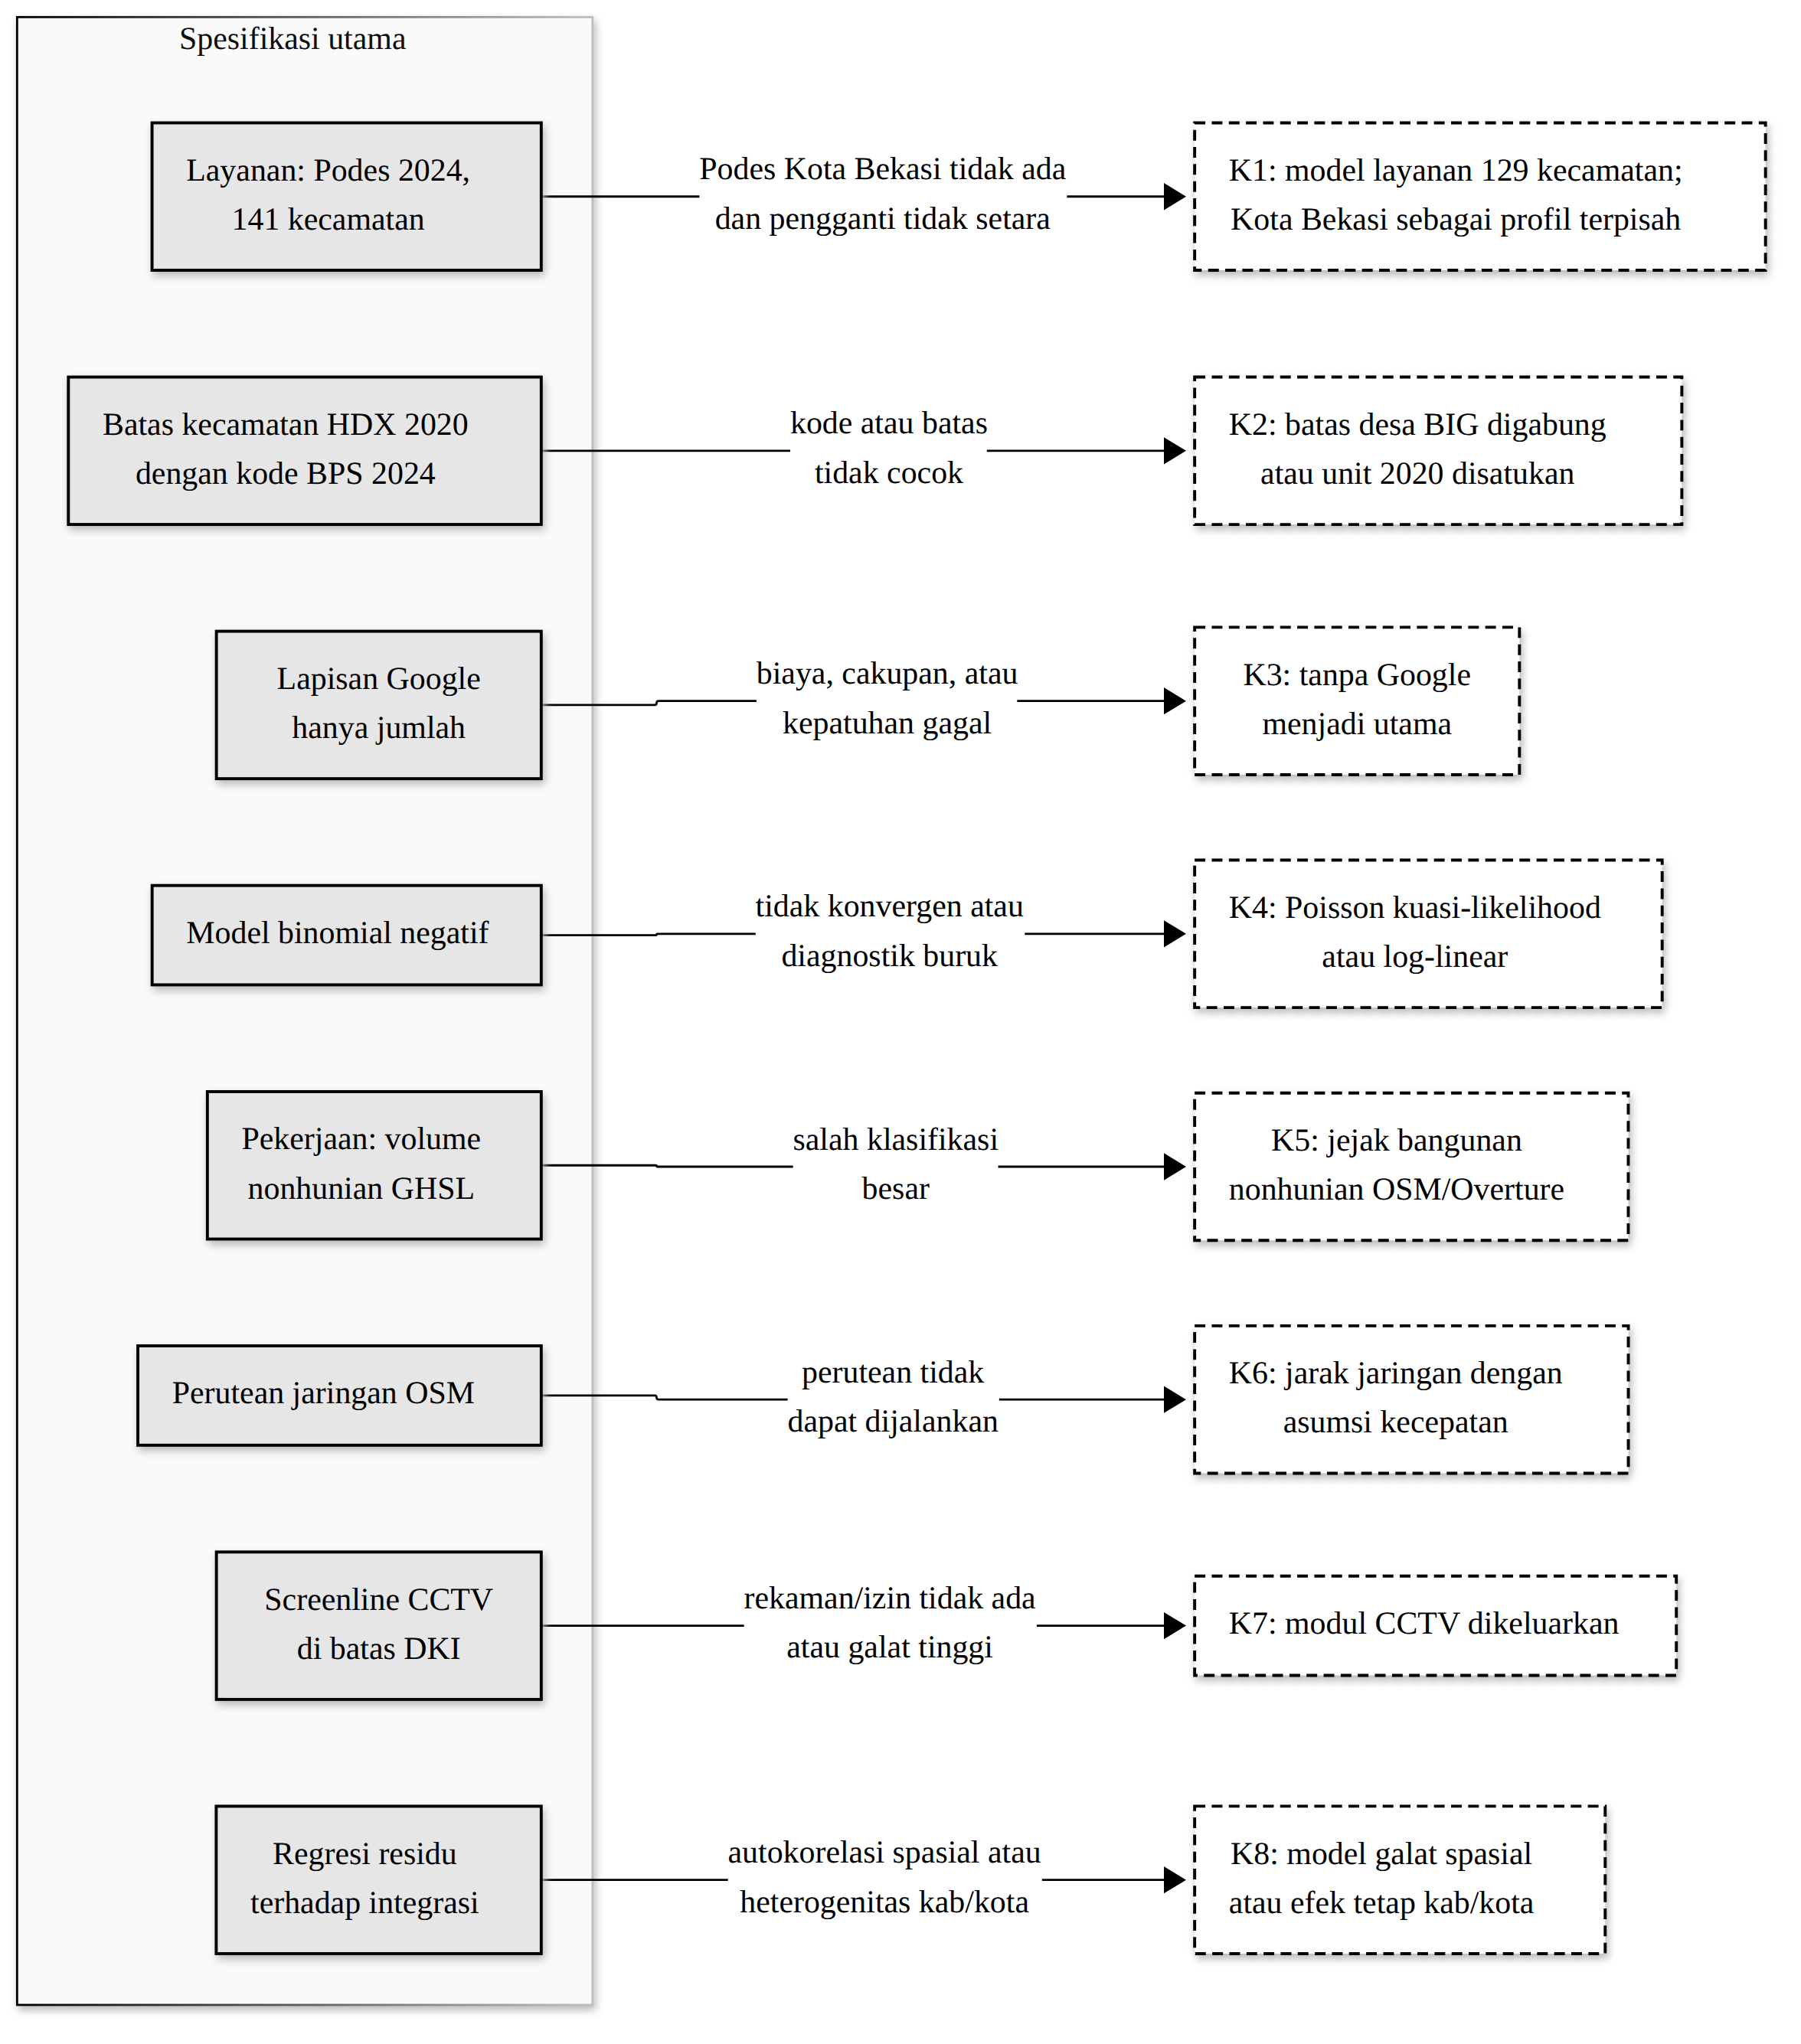
\includegraphics[width=0.8\textwidth]{figures/bab3_keputusan_cadangan.png}
  \caption{Diagram keputusan spesifikasi utama dan cadangan bernama. Setiap cadangan hanya aktif bila pemicunya terpenuhi; selain itu rantai utama dipertahankan.}
  \label{fig:bab3-keputusan-cadangan}
\end{figure}

OD sintetis berbasis model gravitasi, radiasi, atau penyeimbangan IPF
tidak dipakai dalam rantai penelitian. Relasi terarah sudah tersedia
sebagai matriks teramati pada tingkat kabupaten/kota, dan integrasi
tingkat kecamatan tersedia dari WSM. Dengan demikian, risiko sirkular
akibat memakai massa tujuan sebagai masukan relasi tidak muncul.

\subsection{Urutan kerja penelitian}\label{urutan-kerja-penelitian}

Penelitian dilaksanakan melalui delapan langkah yang diuraikan pada
Subbab \ref{metode-analisis-data}:

\begin{enumerate}
\tightlist
\item
  audit sumber dan pembekuan garis dasar;
\item
  penandaan pusat sekunder berdasarkan massa;
\item
  pengukuran integrasi pada kedua tingkat;
\item
  pengukuran fungsi, fungsi harapan, dan residu per domain;
\item
  pengukuran manfaat dan beban dengan indikator terpisah;
\item
  inferensi kemiringan Q3, gerbang bukti, dan tipologi ringkasan;
\item
  diagnostik spasial dan uji ketahanan; serta
\item
  penyusunan keluaran, termasuk Web GIS dan eksplorasi \emph{what-if}.
\end{enumerate}

\begin{figure}[H]
  \centering
  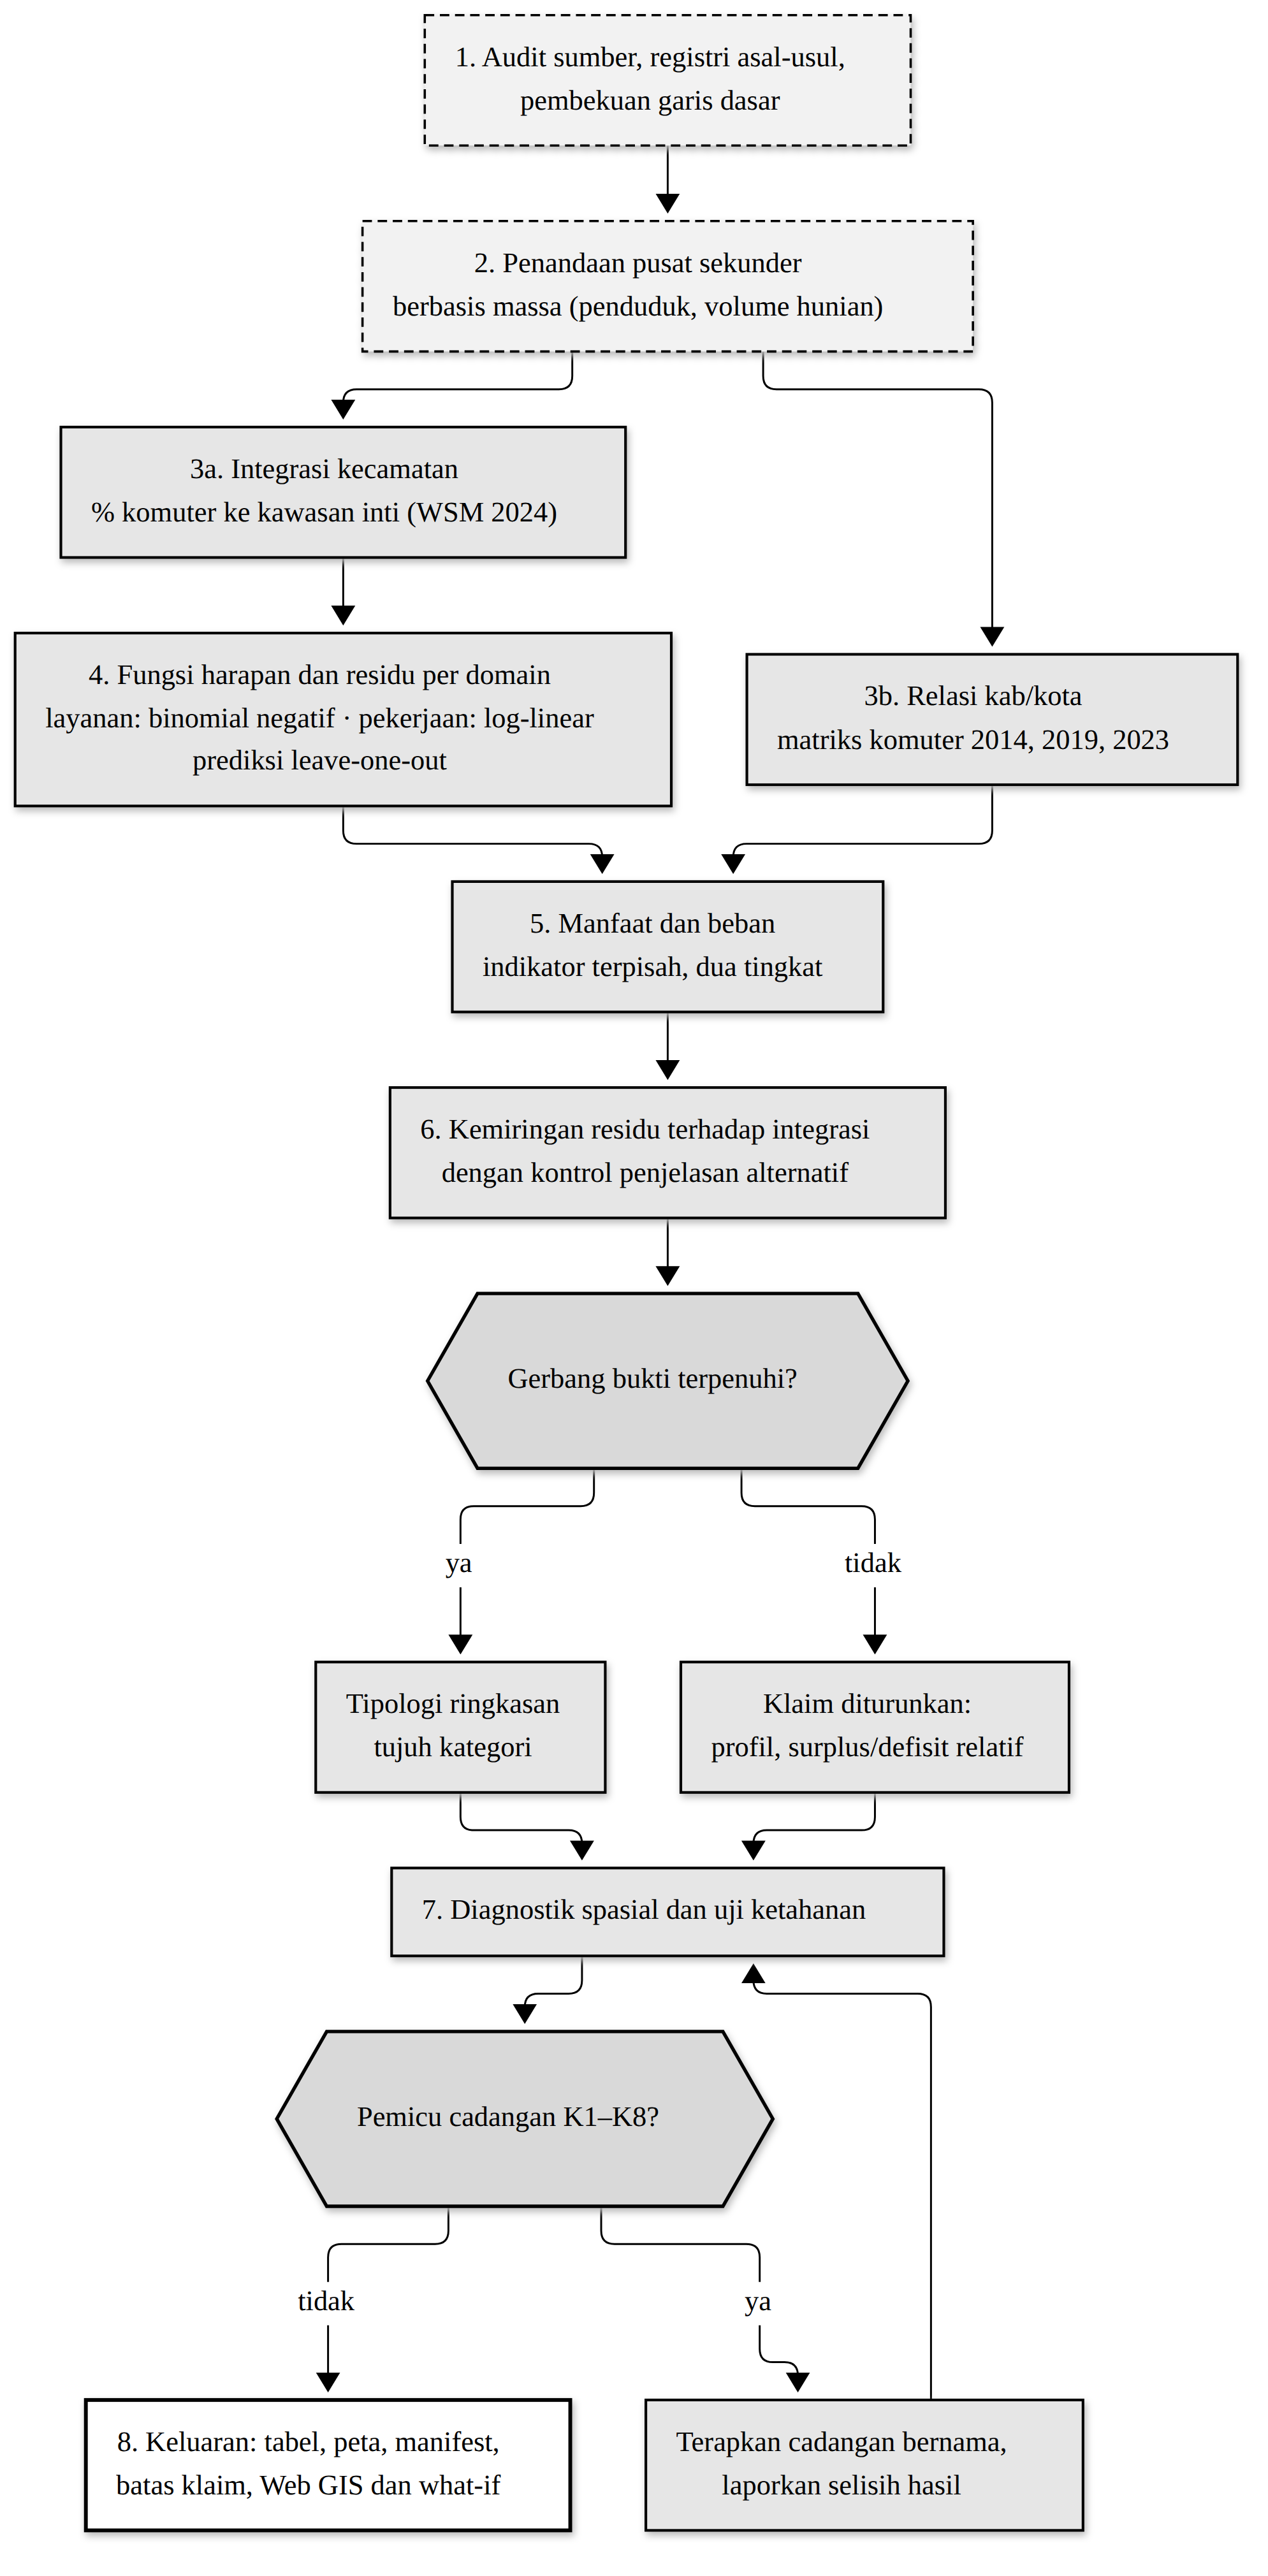
\includegraphics[width=0.6\textwidth]{figures/bab3_alur_analisis.png}
  \caption{Alur analisis dua tingkat dari audit sumber hingga keluaran. Gerbang bukti dapat menurunkan tingkat klaim, dan cadangan bernama hanya dipakai bila pemicunya terpenuhi.}
  \label{fig:bab3-alur-analisis}
\end{figure}

\subsection{Kelebihan dan keterbatasan
desain}\label{kelebihan-dan-keterbatasan-desain}

Desain ini memungkinkan seluruh 141 kecamatan non-DKI dianalisis
dengan sumber terbuka yang seragam cakupannya, tanpa menunggu akses
kelembagaan atau membeli mikrodata. Keterbatasan data resmi maupun
nonpemerintah dinilai secara simetris.

Keterbatasan utamanya adalah ketidaksejajaran unit dan waktu. Relasi
terarah hanya tersedia pada tingkat kabupaten/kota. Volume terbangun
GHSL epoch 2020 merupakan hasil interpolasi dengan observasi terdekat
2018, sehingga berselisih sekitar enam tahun dari Podes dan WSM 2024.
Persentase komuter WSM menuju kawasan inti morfologis, bukan khusus
DKI. Jumlah fasilitas bukan kapasitas atau mutu layanan. Keterbatasan
ini dikelola melalui pelabelan status bukti, uji sensitivitas, dan
pembatasan klaim, bukan dengan menyamarkannya.

\subsection{Perbedaan diagnosis dan
skenario}\label{perbedaan-diagnosis-dan-skenario}

Nilai \emph{status quo} dibekukan sebagai garis dasar. Perubahan
parameter tidak boleh menimpa nilai observasi, mengubah batas
administratif, atau disajikan sebagai prediksi. Perubahan karena
sumber bertambah, hilang, atau turun mutu dicatat sebagai skenario
bukti. Perubahan bobot, ambang, atau spesifikasi dalam konfigurasi bukti
yang sama dicatat sebagai skenario parameter. Perubahan nilai indikator
untuk pertanyaan \emph{what-if} merupakan eksplorasi kondisional.
Ketiganya tidak ditampilkan sebagai jenis perubahan yang sama.

\section{Ruang lingkup penelitian}\label{ruang-lingkup-penelitian}

\subsection{Ruang lingkup spasial}\label{ruang-lingkup-spasial}

Wilayah studi adalah Jabodetabek administratif: DKI Jakarta, Kabupaten
Bogor, Kota Bogor, Kota Depok, Kabupaten Tangerang, Kota Tangerang, Kota
Tangerang Selatan, Kabupaten Bekasi, dan Kota Bekasi. Tolok ukur fungsi
dibentuk dari 141 kecamatan non-DKI di wilayah tersebut, tanpa
pembanding eksternal. DKI Jakarta diperlakukan sebagai satu inti pada
analisis relasi eksternal, dengan batas administratif tetap. Rincian
lima kota administrasi DKI hanya digunakan pada matriks komuter tingkat
2.

Kabupaten Cianjur termasuk Kawasan Aglomerasi menurut UU 2/2024
\parencite{uu22024}, tetapi tidak dicakup. Cianjur berada pada lapisan
luar sistem metropolitan dan tidak tercakup dalam Survei Komuter
Jabodetabek, sehingga unit relasinya tidak sebanding. Penelitian ini
menduga pola yang ditemukan juga relevan bagi Cianjur dengan intensitas
lebih kecil, tetapi dugaan tersebut merupakan alasan pembatasan lingkup,
bukan temuan empiris.

Istilah \emph{Wilayah Statistik Metropolitan} (WSM) merujuk pada
delineasi BPS berdasarkan kawasan inti perkotaan morfologis dan
proporsi komuter dari data posisi ponsel Agustus 2024
\parencite{bpswsm2024}. Kawasan Inti Perkotaan 1 WSM Jabodetabekpunjur
mencakup seluruh DKI Jakarta, Kota Bekasi, Kota Depok, Kota Tangerang,
dan Kota Tangerang Selatan, serta kecamatan padat di Kabupaten Bekasi,
Tangerang, dan Bogor. Delineasi WSM dipakai sebagai salah satu sumber
pengukuran, bukan sebagai pengganti inti penelitian. Inti penelitian
tetap DKI Jakarta.

Wilayah di luar DKI tidak disebut ``wilayah Jakarta'' hanya karena
tercakup dalam gradien analisis. Jejak fungsional yang melintasi batas
dibaca sebagai hubungan metropolitan, bukan zonasi legal atau perluasan
kewenangan.

\subsection{Ruang lingkup temporal}\label{ruang-lingkup-temporal}

Tahun rujukan analisis fungsi adalah 2024, sejajar dengan Podes 2024,
WSM Agustus 2024, dan penduduk 2024. Volume terbangun GHSL memakai epoch
2020 (interpolasi dengan observasi terdekat 2018) dan dibaca sebagai
potret kapasitas fisik, bukan seri waktu. Edisi 2025 publikasi
Statistik Potensi Desa, yang bersumber dari Pemutakhiran Data
Perkembangan Desa 2025, hanya dipakai untuk memeriksa stabilitas jumlah
fasilitas.

Perubahan antarperiode hanya dianalisis pada sisi relasi, yaitu matriks
komuter 2014, 2019, dan 2023. Ketiga edisi berbeda dalam rumusan
definisi komuter, bulan pencacahan, dan kerangka sampel, sehingga
perubahan dibaca sebagai perubahan estimasi survei yang perlu
ditafsirkan hati-hati. Tiga titik waktu tidak disebut tren tahunan.
Perubahan fungsi tidak diklaim karena tidak ada seri fungsi tingkat
kecamatan yang sebanding.

\subsection{Ruang lingkup
substantif}\label{ruang-lingkup-substantif}

Penelitian mencakup:

\begin{itemize}
\tightlist
\item
  integrasi metropolitan pada tingkat kecamatan dan relasi terarah pada
  tingkat kabupaten/kota;
\item
  dua domain fungsi utama, yaitu layanan berorde tinggi dan pekerjaan,
  yang diukur dan diuji terpisah;
\item
  manfaat dan beban yang diukur dengan indikator yang tidak dipakai untuk
  integrasi maupun fungsi;
\item
  inferensi kemiringan residu terhadap integrasi serta tipologi ringkasan
  dengan tujuh kategori yang sama dengan Tabel \ref{tab:tipologi}; serta
\item
  penyajian hasil dalam tabel dan peta, dengan Web GIS sebagai media
  komunikasi.
\end{itemize}

Penelitian tidak mencakup penetapan radius geometris Jakarta,
rekomendasi perubahan batas administrasi, pembuktian kausal kebijakan
metropolitan, atau klaim produktivitas. Kematangan berarti kematangan
fungsi lokal pada dua domain yang diukur, bukan kesejahteraan,
keterjangkauan, mutu layanan, atau keberhasilan pembangunan.

\section{Unit amatan dan unit
analisis}\label{unit-amatan-dan-unit-analisis}

\subsection{Unit amatan}\label{unit-amatan}

Unit amatan adalah satuan tempat observasi dicatat pada sumber. Tingkat
1 memakai kecamatan dengan kode wilayah BPS 2024 sebagaimana tercantum
pada Lampiran 3 dan 13 WSM 2024. Rinciannya adalah Kabupaten Bogor 40
kecamatan, Kabupaten Bekasi 23, Kota Bogor 6, Kota Bekasi 12, Kota Depok
11, Kabupaten Tangerang 29, Kota Tangerang 13, dan Kota Tangerang Selatan
7. Raster GHSL, titik fasilitas, dan titik OSM diagregasikan ke poligon
kecamatan. Tingkat 2 memakai 13 kabupaten/kota sesuai tabulasi Survei
Komuter Jabodetabek. Kabupaten Administrasi Kepulauan Seribu tidak
tampil dalam matriks tersebut.

\subsection{Unit analisis dan penandaan pusat sekunder berbasis
massa}\label{unit-analisis-substantif}

Seluruh 141 kecamatan non-DKI dianalisis. Analisis tidak dibatasi pada
daftar kandidat yang dipilih dari fungsi, karena pemilihan semacam itu
akan menyaring unit berdasarkan variabel hasil. Kecamatan berpenduduk
besar tetapi berfungsi sedikit, yang justru dapat menjadi korban
\emph{shadow}, tetap masuk analisis.

Pusat sekunder ditandai sebagai subkelompok berdasarkan massa saja.
Sebuah kecamatan ditandai sebagai \emph{pusat sekunder berbasis massa}
apabila jumlah penduduknya berada pada kuartil teratas distribusi 141
kecamatan non-DKI, atau volume terbangun huniannya berada pada kuartil
teratas distribusi yang sama. Volume terbangun hunian adalah volume
terbangun total GHSL dikurangi volume nonhunian. Ambang ini ditetapkan
dan dibekukan sebelum fungsi dihitung. Persentil ke-66 dan ke-80 diuji
sebagai sensitivitas. Kecamatan yang berdekatan tidak digabung pada
spesifikasi utama.

Penandaan ini tidak menyatakan bahwa kecamatan lain bukan bagian dari
sistem metropolitan. Fungsinya adalah membaca apakah kemiringan
hubungan integrasi--residu berbeda pada kecamatan bermassa besar. Kawasan
hunian berpenduduk besar diperlakukan sebagai kemungkinan korban
\emph{shadow}, bukan dikecualikan dari analisis.

\subsection{Aturan keterbandingan
unit}\label{aturan-keterbandingan-unit}

Setiap indikator dicatat dengan unit asli, unit perhitungan, unit
pelaporan, dan operasi transformasinya. Harmonisasi mengikuti aturan
berikut:

\begin{enumerate}
\tightlist
\item
  gunakan unit asli untuk perhitungan awal;
\item
  gunakan tabel korespondensi kode resmi bila tersedia;
\item
  agregasikan unit rinci ke unit yang lebih kasar bila operasi tersebut
  sah;
\item
  jalankan analisis paralel bila unit tidak dapat disetarakan;
\item
  keluarkan modul jika keterbandingan tidak dapat dipertanggungjawabkan;
  dan
\item
  jangan membandingkan skor lintas konfigurasi bukti sebagai perubahan
  kondisi tanpa menyatakan perbedaan sumber dan unitnya.
\end{enumerate}

\subsection{Populasi, cakupan, dan validasi
manual}\label{populasi-cakupan-dan-validasi-manual}

Populasi tingkat 1 adalah seluruh 141 kecamatan non-DKI, sehingga tidak
ada sampel statistik tambahan. Untuk domain layanan, populasi efektif
spesifikasi utama dapat menjadi 129 kecamatan bila cadangan K1 berlaku.
Fungsi harapan setiap kecamatan diperkirakan dari kecamatan lain dengan
prosedur \emph{leave-one-out}, agar kecamatan yang sedang dinilai tidak
menentukan ekspektasinya sendiri. Hasilnya adalah posisi relatif di dalam
Jabodetabek.

Pemeriksaan manual dilakukan secara purposif. Lokasi rumah sakit dan
perguruan tinggi diperiksa pada sampel kecamatan yang mencakup
kabupaten dan kota, koridor timur dan barat, serta tingkat integrasi
rendah dan tinggi. Kriteria sampel dicatat sebelum pemeriksaan.
Validasi ini bukan sampel inferensial dan tidak digeneralisasikan
sebagai sensus.

\section{Metode pengumpulan data}\label{metode-pengumpulan-data}

\subsection{Prinsip pengumpulan
data}\label{prinsip-pengumpulan-data}

Penelitian ini bertumpu pada proksi dan sumber terbuka, tanpa
ketergantungan pada permohonan data tertutup atau pembelian mikrodata.
Data pemerintah yang terbuka tetap digunakan. Pemilihan sumber mengikuti
kesesuaian konstruk, cakupan spasial dan temporal, keterulangan
pengolahan, serta biaya pemerolehan. Status resmi tidak menjadi ukuran
mutu dengan sendirinya, dan keunggulan sumber alternatif diuji per
konstruk.

Akuisisi mengikuti jalur yang benar-benar dapat digunakan: unduhan
publikasi, layanan data terbuka, antarmuka pemrograman yang sah, dan
ekstraksi tabel dengan locator halaman. Banyak tabel publikasi BPS
berupa gambar. Tabel semacam itu dibaca secara visual atau dengan OCR,
dan angkanya dicocokkan dengan baris atau kolom total sebelum dipakai.
Terlihat publik tidak berarti boleh disimpan atau dibagikan ulang.
Kemampuan akuisisi dan reproduksi dicatat per sumber.

\subsection{Sumber data}\label{kelompok-sumber-dan-konstruksi-data}

Tabel \ref{tab:bab3-sumber} memuat sumber yang dipakai beserta status
ketersediaannya per Oktober 2026.

\begingroup
\footnotesize
\begin{longtable}{>{\raggedright\arraybackslash}p{0.27\textwidth} >{\raggedright\arraybackslash}p{0.15\textwidth} >{\raggedright\arraybackslash}p{0.17\textwidth} >{\raggedright\arraybackslash}p{0.33\textwidth}}
\caption{Sumber data dan status ketersediaannya}\label{tab:bab3-sumber}\\
\toprule
Sumber & Periode & Unit & Isi yang dipakai dan status \\
\midrule
\endfirsthead
\toprule
Sumber & Periode & Unit & Isi yang dipakai dan status \\
\midrule
\endhead
\midrule
\multicolumn{4}{r}{\footnotesize Dilanjutkan pada halaman berikutnya}\\
\endfoot
\bottomrule
\endlastfoot
Statistik Komuter Jabodetabek \parencite{bpskomuter2014,bpskomuter2019,bpskomuter2023} & 2014, 2019, 2023 & 13 kab/kota & Matriks asal-tujuan (Tabel 2 setiap edisi); kegiatan utama, lama perjalanan, biaya, dan penghasilan komuter 2023. Tersedia; matriks ketiga edisi sudah dicocokkan dengan total. \\
Wilayah Statistik Metropolitan Indonesia 2024 \parencite{bpswsm2024} & MPD Agustus 2024 & Kecamatan & Persentase komuter menuju kawasan inti (Lampiran 13); penduduk, luas, dan kepadatan (Lampiran 3). Tersedia. \\
Statistik Potensi Desa/Kelurahan 2024 per kab/kota \parencite{bpspodeskabbogor2024,bpspodeskotabogor2024,bpspodesdepok2024,bpspodeskabbekasi2024,bpspodeskabtangerang2024,bpspodeskotatangerang2024,bpspodestangsel2024} & Podes 2024 & Kecamatan & Jumlah fasilitas per kecamatan pada bab infrastruktur. Tersedia untuk tujuh kab/kota; tidak ada untuk Kota Bekasi. \\
Statistik Potensi Desa 2025 per kab/kota & 2025 & Kecamatan & Pemutakhiran 2025; pemeriksa stabilitas jumlah fasilitas. Tersedia; definisi sebagian tabel berubah. \\
\emph{Kota Bekasi Dalam Angka 2025} \parencite{bpskotabekasi2025} dan \emph{Kecamatan Dalam Angka 2025} & 2024 & Kecamatan & Pengganti layanan Kota Bekasi. Tabel kesehatan \emph{Dalam Angka} hanya memuat banyaknya kelurahan yang memiliki fasilitas; \emph{Kecamatan Dalam Angka} belum diunduh. \\
GHSL GHS-BUILT-V R2023A \parencite{ghsl2023builtv} & Epoch 2020 & Sel 3 detik busur & Volume terbangun total dan nonhunian. Tersedia; lisensi CC BY 4.0. \\
Peta Kawasan Industri Eksisting \parencite{kemenperin2025ki} & 2025 & Poligon & 30 rekaman kawasan industri formal di Jabodetabek. Tersedia; lisensi pakai ulang tidak tercantum. \\
Google Maps Platform, Places API & Tangkapan 2026 & Titik, disimpan sebagai jumlah per kecamatan & Layanan bisnis, klinik spesialis, dan tempat kerja. Belum diambil; tunduk pada syarat layanan. \\
OpenStreetMap dan Overture & Tangkapan bertanggal & Titik, garis, poligon & Jaringan jalan dan rel untuk perutean, pemeriksaan kelengkapan, dan masker fasilitas layanan. Belum diunduh untuk seluruh wilayah. \\
GTFS statis TransJakarta \parencite{transjakarta2026gtfs} & Berkas 2026 & Rute dan halte & Waktu tempuh angkutan umum terjadwal sebagai sensitivitas. Tersedia; lisensi belum jelas. \\
SIRS Kemenkes dan PDDikti & Tangkapan 2026 & Fasilitas & Kelas rumah sakit, tempat tidur, dan perguruan tinggi untuk pembobot orde layanan. Belum diambil. \\
Laporan BPTJ \parencite{bptj2024} & Kajian 2023--2024 & 182 kecamatan & Bangkitan dan tarikan perjalanan (Tabel 7.1) sebagai pemeriksa proksi pekerjaan. Tersedia. \\
Keadaan Angkatan Kerja Agustus 2023 \parencite{bpskakdki2024,bpskakjabar2024,bpskakbanten2024} & 2023 & Kab/kota & Penduduk bekerja untuk kalibrasi pekerjaan menurut tempat kerja. Tersedia. \\
Tabel upah dan upah minimum BPS & 2019--2025 & Kab/kota & Konteks manfaat. Tersedia sebagian; upah formal Banten tidak ada. \\
\emph{Dalam Angka} provinsi dan kab/kota; PDRB kab/kota \parencite{bpsdki2025,bpsjabar2025,bpsbanten2025,bpspdrb2025} & 2024 & Kab/kota & Penduduk, kepadatan, PDRB, dan struktur sektor untuk Bab 4. Tersedia. \\
Batas kecamatan HDX COD-AB \parencite{hdxcodab2020} & Batas 2020 & Kecamatan & Geometri untuk agregasi dan peta. Belum diunduh; terlalu besar untuk disimpan di repositori. \\
Rekaman CCTV lalu lintas & Sesuai rekaman & Titik ruas & Hitungan terarah di batas DKI. Sumber, izin, dan cakupan waktu belum dicatat. \\
\end{longtable}
\endgroup

\subsection{Operasionalisasi variabel}\label{operasionalisasi-variabel}

Tabel \ref{tab:bab3-operasionalisasi-t1} dan
\ref{tab:bab3-operasionalisasi-t2} menyajikan operasionalisasi variabel
untuk kedua tingkat. Status D, A, S, dan P dijelaskan pada Subbab
\ref{audit-dan-status-mutu-bukti} dan dibaca relatif terhadap unit pada
tingkat masing-masing. Setiap indikator hanya memegang satu peran.

\begingroup
\footnotesize
\begin{longtable}{>{\raggedright\arraybackslash}p{0.12\textwidth} >{\raggedright\arraybackslash}p{0.27\textwidth} >{\raggedright\arraybackslash}p{0.19\textwidth} >{\raggedright\arraybackslash}p{0.11\textwidth} >{\centering\arraybackslash}p{0.04\textwidth} >{\raggedright\arraybackslash}p{0.15\textwidth}}
\caption{Operasionalisasi variabel tingkat 1: 141 kecamatan non-DKI}\label{tab:bab3-operasionalisasi-t1}\\
\toprule
Konstruk & Indikator & Sumber & Periode & St. & Peran \\
\midrule
\endfirsthead
\toprule
Konstruk & Indikator & Sumber & Periode & St. & Peran \\
\midrule
\endhead
\midrule
\multicolumn{6}{r}{\footnotesize Dilanjutkan pada halaman berikutnya}\\
\endfoot
\bottomrule
\endlastfoot
Massa lokal $S$ & Jumlah penduduk & WSM 2024, Lampiran 3; diperiksa dengan \emph{Dalam Angka} kab/kota & 2024 & D & Garis dasar ekspektasi; penanda pusat \\
 & Volume terbangun hunian (total dikurangi nonhunian) & GHSL R2023A & Epoch 2020 & P & Garis dasar alternatif; penanda pusat \\
Karakteristik lokal $X$ & Kepadatan penduduk; status kota/kabupaten; lereng rata-rata & WSM 2024, Lampiran 3; DEM terbuka & 2024 & D/P & Kovariat ekspektasi, jumlahnya dibatasi \\
Penjelasan alternatif $Z$ & Luas kawasan industri formal; keberadaan kota baru skala besar; tahun pembentukan daerah otonom & Kemenperin 2025; OSM dan literatur; regulasi pembentukan & 2025; -- & D/P & Kontrol Q3 \\
Integrasi $I$ & Persentase komuter menuju Kawasan Inti Perkotaan 1 & WSM 2024, Lampiran 13 & Agustus 2024 & A & Variabel penjelas utama Q3 \\
Fungsi layanan $F_L$ & Jumlah rumah sakit, perguruan tinggi, dan bank umum & Statistik Potensi Desa 2024 & Podes 2024 & D & Hasil, domain layanan \\
 & Kelas rumah sakit dan tempat tidur; perguruan tinggi terakreditasi & SIRS; PDDikti & 2026 & D & Pembobot orde (sensitivitas) \\
 & Jumlah layanan bisnis dan klinik spesialis & Google Places, hanya jumlah per kecamatan & 2026 & P & Hasil tambahan, orde tinggi \\
Fungsi pekerjaan $F_P$ & Volume terbangun nonhunian & GHSL R2023A, komponen NRES & Epoch 2020 & P & Hasil, domain pekerjaan \\
 & Pangsa volume nonhunian di dalam kawasan industri & GHSL dan Kemenperin & -- & P & Pembeda manufaktur \\
 & Jumlah tempat kerja Google; tarikan perjalanan BPTJ & Google Places; BPTJ & 2026; 2023 & D/S & Pemeriksa $F_P$, bukan hasil \\
Fungsi harapan dan residu & $\widehat F_{ik}$ dari $S_i$ dan $X_i$ dengan prediksi \emph{leave-one-out}; $R_{ik}$ selisih logaritmik & Perhitungan & -- & S & Hasil Q2; variabel terikat Q3 \\
Manfaat $A$ & Akses kumulatif ke volume nonhunian dalam 60 menit waktu tempuh jaringan & OSM, perutean, GHSL & 2026 & P & Profil manfaat \\
Beban $D$ & Waktu tempuh jaringan arus bebas ke titik acuan inti DKI & OSM, perutean & 2026 & P & Profil beban; gerbang \emph{shadow} \\
\end{longtable}
\endgroup

\begingroup
\footnotesize
\begin{longtable}{>{\raggedright\arraybackslash}p{0.12\textwidth} >{\raggedright\arraybackslash}p{0.30\textwidth} >{\raggedright\arraybackslash}p{0.18\textwidth} >{\raggedright\arraybackslash}p{0.10\textwidth} >{\centering\arraybackslash}p{0.04\textwidth} >{\raggedright\arraybackslash}p{0.14\textwidth}}
\caption{Operasionalisasi variabel tingkat 2: 13 kabupaten/kota}\label{tab:bab3-operasionalisasi-t2}\\
\toprule
Konstruk & Indikator & Sumber & Periode & St. & Peran \\
\midrule
\endfirsthead
\toprule
Konstruk & Indikator & Sumber & Periode & St. & Peran \\
\midrule
\endhead
\bottomrule
\endlastfoot
Relasi terarah $I$ & Arus $F_{ij}$; intensitas; orientasi ke DKI $O_i$; pangsa arus antarpinggiran; rasio masuk/keluar; asimetri pasangan & Statistik Komuter, Tabel 1--2 & 2014, 2019, 2023 & D & Q1; perubahan antarperiode \\
Arah koridor & Volume kendaraan terarah per jam di titik batas DKI, pagi dan sore, per kelas & Rekaman CCTV, deteksi dan pelacakan objek, sampel hitung manual & Sesuai rekaman & S & Q1 tingkat koridor (opsional) \\
Beban $D$ & Pangsa komuter dengan lama perjalanan $\geq$90 menit; pangsa dengan biaya pergi-pulang $\geq$Rp25.000 per hari & Statistik Komuter 2023, Tabel 20 dan 35 & 2023 & D & Profil beban; pemeriksa beban tingkat 1 \\
Manfaat $A$ & Pangsa komuter bekerja berpenghasilan $\geq$Rp5 juta per bulan & Statistik Komuter 2023, Tabel 51 & 2023 & D & Profil manfaat \\
 & Upah pekerja formal dan informal; upah minimum & Tabel BPS provinsi & 2019--2025 & A & Konteks \\
Pekerjaan menurut tempat kerja & Penduduk bekerja dikurangi komuter bekerja keluar, ditambah komuter bekerja masuk & Keadaan Angkatan Kerja 2023; Statistik Komuter 2023 & 2023 & S & Kalibrasi $F_P$; tidak dipasangkan dengan relasi \\
Fungsi dan residu agregat & Agregasi $F$ dan $R$ tingkat 1 ke kab/kota & Perhitungan & -- & S & Dibaca bersama relasi \\
\end{longtable}
\endgroup

Durasi dan biaya pada publikasi komuter tersedia sebagai distribusi
kelas, bukan rata-rata. Karena itu, beban tingkat 2 dinyatakan sebagai
pangsa komuter pada kelas teratas. Arus masuk menurut kegiatan utama
tidak ditabulasikan per tujuan, sehingga pekerjaan menurut tempat kerja
diestimasi dengan asumsi bahwa komposisi kegiatan arus masuk mengikuti
komposisi kegiatan di daerah asal. Estimasi ini diberi status S.

\textbf{Pemeriksaan independensi.} Integrasi $I$ tidak dipakai dalam
pembentukan $F$. Tarikan perjalanan BPTJ dan pekerjaan menurut tempat
kerja hanya menjadi pemeriksa. Beban $D$ diukur dari waktu tempuh,
durasi, dan biaya, bukan dari orientasi atau ketidakseimbangan arus.
Manfaat tingkat 1 memakai waktu tempuh sebagai hambatan menuju peluang,
sedangkan beban memakai waktu tempuh menuju inti. Keduanya merupakan
konstruksi berbeda, dan korelasinya dilaporkan.

\subsection{Instrumen pengumpulan dan dokumentasi
data}\label{instrumen-pengumpulan-dan-dokumentasi-data}

Karena penelitian menggunakan data sekunder, instrumennya bukan
kuesioner atau panduan wawancara. Instrumen kerja terdiri atas:

\begin{enumerate}
\tightlist
\item
  log akses yang mencatat alamat sumber, tanggal akses, dan syarat
  penggunaan;
\item
  registri asal-usul data, termasuk halaman PDF dan halaman isi setiap
  tabel yang diekstrak;
\item
  kamus data yang memuat definisi variabel, unit, tahun, nilai hilang,
  dan polaritas;
\item
  tabel korespondensi kode dan geometri antarversi;
\item
  manifest konfigurasi bukti dan parameter; serta
\item
  lembar pemeriksaan manual untuk fasilitas dan, bila modul CCTV
  dijalankan, untuk sampel hitungan objek.
\end{enumerate}

Skrip akuisisi, pembersihan, transformasi, dan analisis diperlakukan
sebagai bagian dari instrumen yang dapat direproduksi. Nama perangkat
lunak, versi, parameter, dan tanggal pengolahan dicatat setelah
perangkat benar-benar digunakan.

\subsection{Audit dan status mutu
bukti}\label{audit-dan-status-mutu-bukti}

Setiap berkas dicatat dalam registri asal-usul data menurut sumber,
nama dan versi berkas, tanggal akses, tahun observasi, unit, cakupan,
definisi, metode pembentukan, nilai hilang, lisensi, dan pembatasan
publikasi. Status pengukuran setiap indikator mengikuti Tabel
\ref{tab:bab3-status}.

\begin{table}[H]
\centering
\footnotesize
\caption{Status pengukuran bukti}\label{tab:bab3-status}
\begin{tabularx}{\textwidth}{>{\centering\arraybackslash}p{0.07\textwidth} >{\raggedright\arraybackslash}p{0.15\textwidth} X}
\toprule
Status & Nama & Aturan penggunaan \\
\midrule
D & Langsung & Konstruk teramati pada unit dan periode sasaran dengan mutu memadai. \\
A & Agregat & Konstruk teramati, tetapi unit, waktu, kategori, atau cakupan lebih kasar atau berbeda dari sasaran. \\
S & Sintetis & Nilai diestimasi dari data lain; asumsi, kalibrasi, dan ketidakpastian wajib ditampilkan. \\
P & Proksi & Mengukur gejala terkait, bukan konstruk yang diklaim secara langsung. \\
$\varnothing$ & Dikeluarkan & Tidak tersedia, tidak sebanding, tidak reliabel, atau tidak dapat dipertanggungjawabkan. \\
\bottomrule
\end{tabularx}
\end{table}

Status tersebut menjelaskan cara pengukuran, bukan peringkat mutu
sumber. Pengamatan langsung pada unit publikasi tidak selalu merupakan
pengamatan langsung pada unit penelitian. Persentase komuter WSM,
misalnya, berstatus A karena tujuan arusnya adalah kawasan inti
morfologis yang lebih luas daripada DKI.

\subsection{Harmonisasi spasial dan
temporal}\label{harmonisasi-spasial-dan-temporal}

Harmonisasi dilakukan setelah audit. Kode kecamatan BPS 2024 menjadi
kunci penggabungan tabel. Batas kecamatan diambil dari \emph{Indonesia
Subnational Administrative Boundaries} (COD-AB) di HDX, yang bersumber
dari BPS dengan batas April 2020 \parencite{hdxcodab2020}. Kecamatan
pada publikasi 2024 dicocokkan dengan batas 2020, dan bila terjadi
pemekaran atau perubahan nama, cadangan K2 diterapkan. Raster GHSL
diproyeksikan ke UTM 48S (EPSG:32748) sebelum diagregasikan dengan
bobot luas sel yang jatuh di dalam poligon.

Tahun setiap variabel disimpan bersama nilainya. Variabel dari tahun
berbeda tidak dinormalisasi ulang untuk menyembunyikan selisih tahun.
Disagregasi nilai kabupaten/kota ke kecamatan tidak dilakukan, kecuali
pada uji sensitivitas integrasi yang diberi label estimasi.

\subsection{Konstruksi proksi dan
estimasi}\label{konstruksi-proksi-dan-estimasi}

\textbf{Fungsi pekerjaan.} Proksi utama adalah indeks volume terbangun
nonhunian per kecamatan dari komponen NRES GHS-BUILT-V R2023A, epoch
2020 \parencite{ghsl2023builtv}. Proksi ini diukur dari citra satelit
sehingga cakupannya seragam dan tidak bergantung pada kelengkapan
pemetaan sukarela. Nilainya adalah kapasitas fisik tempat kerja, bukan
jumlah pekerja. Konversi ke jumlah pekerjaan hanya dilakukan melalui
kalibrasi terhadap pekerjaan menurut tempat kerja pada 13
kabupaten/kota dan diberi label estimasi. Kelas nonhunian juga mencakup
rumah sakit, kampus, dan pusat perbelanjaan. Karena itu, uji
sensitivitas mengeluarkan poligon fasilitas layanan OSM dari volume
nonhunian sebelum korelasi antardomain dihitung.

\textbf{Fungsi layanan.} Spesifikasi utama menjumlahkan rumah sakit,
akademi/perguruan tinggi, dan bank umum per kecamatan dari tabel
infrastruktur publikasi Statistik Potensi Desa 2024. Ketiga jenis ini
mewakili layanan kesehatan, pendidikan tinggi, dan keuangan yang
melayani lebih dari satu kecamatan. Pertokoan, pasar, dan akomodasi
dikeluarkan dari spesifikasi utama karena lebih dekat dengan layanan
harian atau wisata, tetapi diuji sebagai sensitivitas. Nilai nol tetap
ikut dianalisis. Lapisan Google Places menambahkan layanan bisnis dan
klinik spesialis yang tidak dicakup Podes.

\textbf{Kelengkapan OSM.} Kelengkapan pemetaan OSM cenderung lebih tinggi
di kawasan yang lebih urban dan lebih dekat ke Jakarta. Bias ini dapat
menciptakan asosiasi semu antara integrasi dan fungsi. Karena itu,
setiap lapisan OSM diperiksa kelengkapannya per kecamatan terhadap
Overture dan jumlah fasilitas Podes sebelum dipakai.

\textbf{Hitungan CCTV.} Bila rekaman tersedia, CCTV dipakai untuk
\emph{screenline} terarah di titik penyeberangan batas DKI pada koridor
utama, pagi dan sore. Model deteksi objek pralatih mengenali kelas
kendaraan, dan pelacak objek mempertahankan identitas antarbingkai.
Hasilnya divalidasi dengan hitungan manual pada sampel yang mewakili
kamera, kepadatan, cuaca, pencahayaan, dan sudut pandang. Keluarannya
adalah arah dan asimetri volume per koridor. Hitungan ruas bukan
pasangan asal-tujuan, memuat lalu lintas tembus, dan memerlukan asumsi
okupansi untuk dikonversi ke orang. SUMO hanya dipakai bila
dikombinasikan dengan hitungan CCTV untuk simulasi koridor pada
eksplorasi \emph{what-if}. Statusnya penguatan opsional.

\subsection{Etika, lisensi, dan
keamanan}\label{etika-lisensi-dan-keamanan}

\textbf{Google Maps Platform.} Data Google hanya dipakai untuk
menghitung. Syarat layanan Places API mengizinkan \emph{place ID}
disimpan tanpa batas waktu, membatasi penyimpanan koordinat paling lama
30 hari, dan tidak mengizinkan atribut lain disimpan sebagai basis data
\parencite{googlemaps2026terms}. Desain kepatuhannya adalah sebagai
berikut:

\begin{enumerate}
\tightlist
\item
  titik dari Places API langsung ditumpangkan ke poligon kecamatan dalam
  proses yang sama, jauh di bawah batas 30 hari;
\item
  yang disimpan hanya tabel \texttt{place\_id | kode\_kecamatan |
  kategori\_penelitian}, skrip, tanggal pengambilan, dan daftar jenis
  tempat yang dicari, sedangkan koordinat, nama, dan alamat tidak
  disimpan;
\item
  deduplikasi antarpotongan area pencarian memakai \emph{place ID};
\item
  Web GIS hanya menampilkan agregat per kecamatan, bukan titik Google;
  dan
\item
  berbagi data dilakukan dalam bentuk tabel agregat dan daftar
  \emph{place ID}.
\end{enumerate}

Penyimpanan pasangan \emph{place ID} dengan kode kecamatan dan kategori
buatan sendiri merupakan wilayah abu-abu dalam syarat layanan dan
dinyatakan terbuka di sini. Pengambilan ulang lewat \emph{place ID}
dapat menghasilkan isi yang berubah, sehingga reproduktibilitasnya
terbatas. Uji coba dilakukan pada satu kabupaten/kota untuk mengukur
jumlah panggilan sebelum seluruh Jabodetabek diproses.

\textbf{Lisensi lain.} GHSL berlisensi CC BY 4.0. Batas COD-AB HDX
berlisensi CC BY-IGO. Status lisensi GTFS TransJakarta dan data kawasan
industri Kemenperin belum tercantum, sehingga keduanya hanya dipakai
untuk analisis dan ditampilkan dalam bentuk turunan dengan atribusi.

\textbf{CCTV.} Pengolahan CCTV hanya menyimpan hitungan agregat dan
metadata yang diperlukan, bukan wajah, pelat nomor, atau identitas
individu. Sumber rekaman, izin, dan cakupan waktunya dicatat sebelum
modul dijalankan.

\section{Metode analisis data}\label{metode-analisis-data}

\subsection{Langkah 1: audit, dokumentasi, dan pembekuan garis
dasar}\label{langkah-1-audit-dokumentasi-dan-pembekuan-garis-dasar}

Analisis dimulai dengan tabel audit yang menghubungkan konstruk,
indikator, sumber, tahun, unit, polaritas, status bukti, aturan
transformasi, dan batas klaim. Indikator yang dikeluarkan karena
duplikasi, cakupan tidak memadai, nilai hilang, ketidakcocokan unit,
atau definisi yang tidak jelas dicatat sebagai keputusan metodologis.
Garis dasar dibekukan setelah audit.

\subsection{Langkah 2: penandaan pusat sekunder berbasis
massa}\label{langkah-2-delineasi-pusat-sekunder-dan-wilayah-tangkapan-fungsional}

Ambang massa pada Subbab \ref{unit-analisis-substantif} diterapkan pada
penduduk dan volume terbangun hunian sebelum fungsi dihitung. Daftar
kecamatan yang ditandai, ambangnya, dan tanggal pembekuannya disimpan
dalam manifest. Penandaan ini tidak memakai jumlah fasilitas, volume
nonhunian, kawasan industri, posisi jaringan, atau arus komuter.

\subsection{Langkah 3: pengukuran integrasi
metropolitan}\label{langkah-3-pengukuran-integrasi-metropolitan}

\textbf{Tingkat 1.} Integrasi kecamatan $I_i$ adalah persentase komuter
menuju Kawasan Inti Perkotaan 1 WSM 2024. Persentase ini dihitung BPS
sebagai jumlah penduduk yang melakukan perjalanan rutin ke kawasan inti
dibagi total penduduk bekerja dan sekolah di wilayah asal, berdasarkan
data posisi ponsel Agustus 2024 \parencite{bpswsm2024}. Nilainya
tersedia untuk seluruh 141 kecamatan, dengan rentang 1,9--47,8 persen.
Kelas delineasi WSM (inti, periferi, bukan WSM) tidak dipakai sebagai
kebenaran dasar, dan yang dipakai adalah nilai kontinu. Tujuan arus ini
mencakup DKI beserta hamparan inti morfologis di sekitarnya. Karena itu,
uji sensitivitas memakai integrasi khusus DKI hasil estimasi:

\[
I^{\mathrm{DKI}}_i = I_i \times O_{k(i)}^{2023},
\]

\noindent dengan $O_{k(i)}^{2023}$ sebagai pangsa komuter
kabupaten/kota $k$, tempat kecamatan $i$ berada, yang menuju DKI pada
matriks komuter 2023. Estimasi ini berstatus S karena mengasumsikan
pangsa tujuan yang sama di seluruh kecamatan dalam satu kabupaten/kota.

\textbf{Tingkat 2.} Dari matriks komuter $F_{ij}$, dengan $i$ sebagai
tempat tinggal dan $j$ sebagai lokasi kegiatan, dihitung lima profil
relasi untuk setiap edisi:

\[
O_i = \frac{\sum_{j \in J} F_{ij}}{\sum_{j \neq i} F_{ij}}, \qquad
P_i = \frac{\sum_{j \in B,\, j \neq i} F_{ij}}{\sum_{j \neq i} F_{ij}}, \qquad
M_i = \frac{\sum_{j \neq i} F_{ji}}{\sum_{j \neq i} F_{ij}}, \qquad
\mathrm{AS}_{ij} = \frac{F_{ij}-F_{ji}}{F_{ij}+F_{ji}},
\]

\noindent dengan $J$ sebagai lima kota administrasi DKI dan $B$ sebagai
delapan kabupaten/kota Bodetabek. $O_i$ adalah orientasi ke DKI, $P_i$
pangsa arus antarpinggiran, $M_i$ rasio arus masuk terhadap keluar, dan
$\mathrm{AS}_{ij}$ asimetri pasangan. Intensitas komuter adalah
persentase komuter terhadap penduduk berumur 5 tahun ke atas pada
Tabel 1 setiap edisi. Kolom ``Luar Jabodetabek'' dilaporkan terpisah.
Hitungan CCTV, bila tersedia, dibaca sebagai arah dan asimetri koridor
dan tidak dicampur dengan matriks.

Waktu tempuh dan konektivitas jaringan tidak dipakai sebagai integrasi.
Keduanya hanya muncul pada manfaat dan beban (Langkah 5).

\subsection{Langkah 4: pengukuran fungsi lokal dan fungsi
relatif}\label{langkah-4-pengukuran-fungsi-lokal-dan-fungsi-relatif}

Fungsi relatif dihitung terpisah untuk domain layanan ($k=L$) dan
pekerjaan ($k=P$). Untuk layanan, yang berupa data hitungan dengan nilai
nol dan sebaran berlebih, fungsi harapan dimodelkan dengan regresi
binomial negatif:

\[
\ln \mathrm{E}[F_{iL}] = \alpha_L + \beta_L \ln S_i + \boldsymbol{\gamma}_L^{\mathsf T}\mathbf{X}_i .
\]

\noindent Untuk pekerjaan, yang berupa volume kontinu, dipakai model
log-linear:

\[
\ln F_{iP} = \alpha_P + \beta_P \ln S_i + \boldsymbol{\gamma}_P^{\mathsf T}\mathbf{X}_i + \varepsilon_{iP}.
\]

Kedua model diestimasi dengan prosedur \emph{leave-one-out}: harapan
$\widehat F_{(-i)k}$ untuk kecamatan $i$ diprediksi dari model yang
diestimasi tanpa kecamatan $i$. Residu fungsi didefinisikan sebagai

\[
R_{ik} = \ln(F_{ik} + c_k) - \ln\bigl(\widehat F_{(-i)k} + c_k\bigr),
\]

\noindent dengan $c_L = 0{,}5$ untuk hitungan layanan dan $c_P = 0$
untuk volume. Residu positif berarti surplus relatif dan residu negatif
berarti defisit relatif terhadap kecamatan non-DKI lain dengan massa dan
karakteristik serupa. Integrasi $I$ dan penjelasan alternatif $Z$ tidak
dimasukkan ke model ekspektasi, sehingga residu tidak dibentuk dari
variabel penjelas Q3.

Karena ekspektasi dibentuk secara internal, residu berpusat di sekitar
nol menurut konstruksinya. Tanda residu satu kecamatan karena itu tidak
menjadi bukti \emph{shadow} atau \emph{borrowed size}. Bukti tersebut
dibaca dari hubungan residu dengan integrasi pada Langkah 6. Residu
layanan tidak disebut produktivitas, dan residu volume nonhunian tidak
disebut jumlah pekerjaan.

\subsection{Langkah 5: pengukuran manfaat dan beban}\label{langkah-5-pemisahan-manfaat-ketergantungan-dan-beban}

Manfaat dan beban tidak dilebur menjadi satu skor bersih, dan residu
fungsi tidak dihitung kembali sebagai manfaat atau beban.

\textbf{Tingkat 1.} Manfaat adalah akses kumulatif ke peluang kerja:

\[
A_i = \sum_{j} V_j \,\mathbf{1}\bigl(t_{ij} \leq 60\ \text{menit}\bigr),
\]

\noindent dengan $V_j$ sebagai volume nonhunian sel $j$ di seluruh
Jabodetabek, termasuk DKI, dan $t_{ij}$ sebagai waktu tempuh jaringan
arus bebas dari titik berat penduduk kecamatan $i$ hasil perutean OSM.
Ambang 45 dan 90 menit diuji sebagai sensitivitas. Beban adalah waktu
tempuh jaringan arus bebas dari titik berat penduduk kecamatan ke titik
acuan inti DKI, yaitu Bundaran Hotel Indonesia, dengan waktu tempuh ke
kecamatan DKI terdekat sebagai sensitivitas. Waktu tempuh terjadwal GTFS
TransJakarta dipakai sebagai pemeriksa moda angkutan umum. Keduanya
berstatus P karena kemacetan tidak terekam dalam jaringan OSM.

\textbf{Tingkat 2.} Beban adalah pangsa komuter dengan lama perjalanan
sedikitnya 90 menit dan pangsa komuter dengan biaya pergi-pulang
sedikitnya Rp25.000 per hari menurut kabupaten/kota asal. Manfaat adalah
pangsa komuter bekerja yang berpenghasilan sedikitnya Rp5 juta per
bulan. Upah dan upah minimum kabupaten/kota menjadi konteks. Beban
tingkat 2 juga dipakai untuk memeriksa apakah urutan beban potensial
tingkat 1, setelah diagregasikan, sejalan dengan beban yang dialami.

Integrasi tinggi lazimnya berasosiasi dengan waktu tempuh ke inti yang
lebih pendek. Karena itu, syarat ``beban tinggi'' pada gerbang
\emph{shadow} dinilai di antara kecamatan dengan tingkat integrasi
serupa, bukan pada seluruh sebaran. Polaritas ditetapkan per konstruk
dan tidak disimpulkan dari tanda mentah.

\subsection{Langkah 6: inferensi kemiringan, gerbang bukti, dan
tipologi}\label{langkah-6-diagnosis-tipologi-dan-gradien}

\textbf{Inferensi utama Q3.} Untuk setiap domain $k$, residu diregresikan
terhadap integrasi:

\[
R_{ik} = a_k + \theta_k I_i + \boldsymbol{\delta}_k^{\mathsf T}\mathbf{Z}_i + u_{ik}.
\]

\noindent Estimand utama adalah kemiringan $\theta_k$. Kemiringan negatif
yang stabil konsisten dengan \emph{agglomeration shadow} pada domain
$k$, sedangkan kemiringan positif yang stabil konsisten dengan
\emph{borrowed size}. Kesimpulan tidak diambil dari banyaknya kecamatan
yang residunya negatif. Galat baku dihitung dengan estimator yang tahan
heteroskedastisitas. Jumlah kovariat $Z$ dibatasi agar sebanding dengan
jumlah kecamatan efektif. Tiga variasi diperiksa: interaksi $I$ dengan
penanda pusat berbasis massa, untuk menguji apakah kemiringan berbeda
pada kecamatan bermassa besar; bentuk tak linear $I$ melalui
\emph{spline}; dan model satu tahap $\ln F$ terhadap $S$, $X$, $I$, dan
$Z$ sebagai pembanding prosedur dua tahap. Pada tingkat 2, hubungan
antara residu agregat dan relasi dibaca sebagai profil, bukan regresi,
karena hanya terdapat delapan unit non-DKI.

\textbf{Gerbang bukti.} Label ketat \emph{borrowed size} atau
\emph{agglomeration shadow} hanya dipakai bila empat syarat terpenuhi:

\begin{enumerate}
\tightlist
\item
  terdapat bukti relasional teramati, bukan hanya jarak atau waktu
  tempuh;
\item
  fungsi aktual dibandingkan dengan ekspektasi dari massa pada unit yang
  memadai;
\item
  relasi dan fungsi dihubungkan pada unit dan periode yang cukup
  sebanding; dan
\item
  arah kemiringan tidak berubah pada uji ketahanan utama dan tidak
  bergantung pada satu proksi lemah.
\end{enumerate}

Khusus \emph{agglomeration shadow}, kemiringan negatif harus disertai
beban yang diukur terpisah dari integrasi maupun residu. Tanpa bukti
tersebut, hasilnya disebut ``terintegrasi tetapi tertinggal''.

\textbf{Tipologi ringkasan.} Setelah gerbang bukti, setiap kecamatan
dapat diringkas ke dalam tujuh kategori yang sama dengan Tabel
\ref{tab:tipologi}. Integrasi dikategorikan tinggi atau rendah dengan
ambang yang dibekukan sebelum klasifikasi, yaitu median $I$ pada
spesifikasi utama dan tersier sebagai sensitivitas. Residu disebut
positif atau negatif hanya bila selang ketidakpastiannya tidak memuat
nol. Unit yang tidak memenuhi syarat itu, atau kelasnya berubah pada
spesifikasi utama, masuk kategori ``tidak terselesaikan''. Tipologi
menggambarkan posisi relatif di dalam Jabodetabek dan tidak menggantikan
inferensi kemiringan.

Istilah \emph{transisional} tidak digunakan, karena perubahan fungsi
antarperiode tidak diamati. Perbedaan antardomain pada satu periode
disebut campuran, sedangkan perubahan kelas akibat spesifikasi disebut
tidak terselesaikan.

\subsection{Langkah 7: diagnostik spasial dan ketahanan
hasil}\label{langkah-7-diagnostik-spasial-dan-ketahanan-hasil}

Autokorelasi spasial residu model Q3 diperiksa dengan Moran's I memakai
matriks ketetanggaan \emph{queen} dan, sebagai pembanding, $k$ tetangga
terdekat. Jika autokorelasi kuat, cadangan K8 diterapkan. Model spasial
merupakan penguatan, bukan syarat desain minimum.

Uji ketahanan berikut dijalankan pada garis dasar yang sama:

\begin{enumerate}
\tightlist
\item
  garis dasar massa: penduduk atau volume terbangun hunian;
\item
  pembanding: prediksi \emph{leave-one-out} atau tetangga ukuran
  terdekat;
\item
  bentuk residu: konstanta $c_L$ dan residu \emph{deviance};
\item
  masker fasilitas layanan OSM pada volume nonhunian GHSL;
\item
  komposisi layanan: per jenis fasilitas, dengan pertokoan dan
  akomodasi, serta pembobotan kelas SIRS/PDDikti;
\item
  jumlah fasilitas Podes 2025 sebagai pengganti Podes 2024;
\item
  integrasi khusus DKI hasil estimasi $I^{\mathrm{DKI}}$;
\item
  kemiringan di dalam kabupaten/kota (efek tetap);
\item
  ambang tipologi dan ambang massa; serta
\item
  analisis tanpa lapisan Google.
\end{enumerate}

Ketahanan tidak diringkas hanya sebagai persentase kelas yang sama.
Rentang kemiringan, peta perpindahan kelas, dan daftar unit tidak
terselesaikan ditampilkan bersama alasannya.

\subsection{Langkah 8: penyusunan keluaran, Web GIS, dan eksplorasi
\emph{what-if}}\label{langkah-8-penyusunan-keluaran-dan-penguatan-opsional}

Keluaran inti terdiri atas tabel audit dan manifest mutu bukti, peta dan
profil relasi kedua tingkat, peta residu per domain, estimasi kemiringan
beserta ketidakpastiannya, profil manfaat dan beban, tipologi ringkasan,
serta hasil uji ketahanan. Keluaran ini dapat dihasilkan tanpa Web GIS.

Web GIS interaktif dikembangkan sebagai media komunikasi dan eksplorasi
dari model yang sama. Isinya peta garis dasar, peta skenario, peta
selisih, unit yang berpindah kelas, dan peta ketahanan. Lapisan Google
hanya ditampilkan sebagai agregat per kecamatan. Eksplorasi
\emph{what-if} mengubah nilai indikator dalam rentang yang beralasan
untuk membaca konsekuensi kondisional, misalnya penambahan fasilitas
pada kecamatan tertentu terhadap posisi residunya. Skenario bukti,
skenario parameter, dan eksplorasi \emph{what-if} dibedakan dan tidak
disebut prediksi kebijakan. Batas administratif DKI selalu tampil
sebagai lapisan tetap.

\subsection{Keterlacakan pertanyaan
penelitian}\label{keterlacakan-pertanyaan-dan-analisis-asosiasi}

Tabel \ref{tab:bab3-keterlacakan} menghubungkan setiap pertanyaan
dengan analisis dan keluarannya.

\begingroup
\footnotesize
\begin{longtable}{>{\raggedright\arraybackslash}p{0.12\textwidth} >{\raggedright\arraybackslash}p{0.50\textwidth} >{\raggedright\arraybackslash}p{0.30\textwidth}}
\caption{Keterlacakan pertanyaan penelitian ke analisis dan keluaran}\label{tab:bab3-keterlacakan}\\
\toprule
Pertanyaan & Analisis & Keluaran \\
\midrule
\endfirsthead
\toprule
Pertanyaan & Analisis & Keluaran \\
\midrule
\endhead
\bottomrule
\endlastfoot
Q1 & Peta alir dan indeks orientasi, antarpinggiran, rasio masuk/keluar, serta asimetri pasangan dari matriks 13 unit untuk 2014, 2019, dan 2023; peta persentase komuter menuju kawasan inti per kecamatan; volume koridor CCTV bila tersedia & Profil relasi kedua tingkat dan perubahan pada sisi relasi \\
Q2 & Model binomial negatif untuk layanan dan model log-linear untuk volume nonhunian terhadap $S$ dan $X$, dengan prediksi \emph{leave-one-out}; manfaat dan beban pada kedua tingkat & Residu per domain; profil manfaat dan beban \\
Q3 & Regresi residu terhadap $I$ dengan kontrol $Z$ pada tingkat 1; Moran's I residu; model spasial sebagai penguatan; tipologi setelah gerbang bukti; tingkat 2 dibaca sebagai profil & Kemiringan $\theta_k$ per domain dan selang ketidakpastiannya; tipologi ringkasan \\
\end{longtable}
\endgroup

Proposisi P1--P4 di Bab 2 diuji melalui analisis ini. P1 diuji dengan
kemiringan domain layanan, termasuk interaksinya dengan penanda pusat
berbasis massa. P2 diuji dengan profil tingkat 2 dan residu pekerjaan
kecamatan di dalam kawasan industri. P3 diuji dengan korelasi residu
kedua domain. P4 diuji dengan bentuk tak linear $I$.

\subsection{Analisis multitemporal dan batas
keterbandingan}\label{analisis-multitemporal-dan-batas-keterbandingan}

Analisis perubahan hanya dilakukan pada matriks komuter 2014, 2019, dan
2023. Untuk setiap edisi, profil $O_i$, $P_i$, $M_i$, dan asimetri
pasangan dihitung dengan definisi yang sama, lalu dibandingkan. Edisi
2014 dan 2019 mendefinisikan komuter sebagai orang yang bekerja,
sekolah, atau kursus di luar kabupaten/kota tempat tinggal dan pulang
pergi pada hari yang sama. Edisi 2023 merumuskannya sebagai pergerakan
harian melewati batas kabupaten/kota. Bulan pencacahan dan kerangka
sampelnya juga berbeda. Perubahan karena itu dilaporkan bersama catatan
perbedaan definisi, dan perubahan kecil tidak ditafsirkan sebagai
perubahan struktur.

Perubahan fungsi tidak dihitung. GHSL epoch 2020 merupakan interpolasi,
dan edisi 2025 publikasi Statistik Potensi Desa memiliki definisi dan
sumber yang berbeda dari Podes 2024. Perbandingan sumber yang mengubah
konstruk dilaporkan sebagai triangulasi, bukan sensitivitas yang
setara.

\subsection{Validitas, reliabilitas, dan
reproduktibilitas}\label{validitas-reliabilitas-dan-reproduktibilitas}

Validitas konstruk dijaga dengan memisahkan massa lokal, integrasi,
aksesibilitas, fungsi, manfaat, dan beban, serta dengan aturan satu
indikator satu peran. Jumlah fasilitas, volume nonhunian, dan waktu
tempuh tidak diperlakukan sebagai produktivitas, jumlah pekerjaan, atau
integrasi aktual.

Reliabilitas dijaga melalui aturan transformasi yang terdokumentasi,
ambang yang ditetapkan sebelum klasifikasi, dan uji ketahanan pada
Langkah 7. Penghitungan dengan masukan dan parameter yang sama harus
menghasilkan keluaran yang sama. Ketidaksesuaian antarsumber dilaporkan
dan tidak diselesaikan dengan memilih sumber yang menghasilkan
klasifikasi yang diinginkan.

Validitas eksternal dibatasi pada unit, tahun, dan wilayah yang
tercakup. Hasil kabupaten/kota tidak digeneralisasikan ke kecamatan,
dan pola dalam sistem Jakarta tidak dianggap berlaku untuk metropolitan
lain.

Paket reproduksi memuat kamus data, log akses, registri asal-usul data,
geometri dan tabel korespondensi, skrip, nilai garis dasar, parameter
uji ketahanan, daftar data yang dikeluarkan beserta alasannya, serta
manifest keluaran dan syarat penyebarluasannya.

\subsection{Aturan keputusan, keluaran, dan batas
klaim}\label{aturan-keputusan-keluaran-dan-batas-klaim}

Konfigurasi bukti yang lolos audit dibekukan sebelum analisis, dan
perubahan sumber atau model disimpan sebagai versi baru. Jika suatu
modul gagal, cadangan bernama diterapkan sesuai pemicunya, atau batas
modul dilaporkan tanpa mengubah nilai hilang menjadi nol.

Dengan rancangan ini, penelitian dapat menyatakan arah dan besar
hubungan integrasi--fungsi relatif per domain di Jabodetabek, profil
relasi terarah dan perubahannya pada tiga edisi survei, profil manfaat
dan beban, serta stabilitas hasil terhadap asumsi yang diuji. Penelitian
tidak dapat menyatakan bahwa Jakarta secara kausal menyebabkan defisit
fungsi, bahwa satu radius merupakan batas metropolitan yang benar, atau
bahwa perubahan nilai dalam Web GIS memprediksi dampak kebijakan.
Label \emph{borrowed size} dan \emph{agglomeration shadow} digunakan
secara ketat hanya setelah gerbang bukti terpenuhi. Jika tidak, hasil
ditulis sebagai pola yang konsisten atau tidak konsisten dengan konstruk
tersebut pada unit, periode, dan konfigurasi bukti yang disebutkan.

\clearpage

\chapter{Bab 4 Gambaran Umum Lokasi Penelitian}

Bab ini menjelaskan wilayah yang menjadi konteks pengukuran. Uraian disusun untuk membantu pembaca memahami hubungan antara Jakarta, kota-kota di sekitarnya, kabupaten dengan perkembangan perkotaan yang cepat, serta jaringan transportasi yang menghubungkannya. Angka dalam bab ini bersifat deskriptif dan dikutip dari publikasi dengan tahun dan locator yang disebutkan. Bab ini tidak menyajikan diagnosis \emph{borrowed size} atau \emph{agglomeration shadow}; diagnosis tersebut menjadi bagian Bab 5.

\section{Posisi Jabodetabek dalam sistem metropolitan dan kebijakan}

Jabodetabek merupakan kawasan metropolitan yang terbentuk dari hubungan harian antara Jakarta dan wilayah di sekitarnya. Hubungan itu melampaui batas provinsi dan batas kewenangan satu pemerintah daerah. Jakarta berperan sebagai inti dengan konsentrasi fungsi pemerintahan, jasa tingkat tinggi, kegiatan ekonomi, dan simpul transportasi. Bogor, Depok, Tangerang, dan Bekasi menampung perumahan, pekerjaan, industri, pendidikan, perdagangan, serta fasilitas yang tumbuh dengan tingkat kemandirian yang berbeda. Literatur tentang perkembangan Jabotabek mencatat perluasan permukiman sekaligus perubahan struktur pekerjaan, industri, jaringan, dan hubungan antarsubwilayah \parencite{henderson1996,hudalahfirman2012,hudalahetal2013}. Penelitian yang lebih baru menunjukkan tumbuhnya komuter antarpinggiran seiring desentralisasi pekerjaan industri \parencite{sadewoetal2023,aritenang2023}.

Secara kebijakan, Jabodetabek menjadi inti Kawasan Aglomerasi yang dibentuk Undang-Undang Nomor 2 Tahun 2024. Kawasan tersebut mencakup minimal sembilan unit Jabodetabek dan Kabupaten Cianjur. Pembangunannya disinkronkan melalui rencana tata ruang kawasan strategis nasional dan rencana induk pembangunan yang programnya mencakup transportasi, penanggulangan banjir, air minum, infrastruktur wilayah, dan penataan ruang. Koordinasinya dijalankan oleh Dewan Kawasan Aglomerasi \parencite[Pasal 51--55]{uu22024}. Berlakunya undang-undang tersebut dikaitkan dengan penetapan Keputusan Presiden mengenai pemindahan ibu kota negara \parencite[Pasal 73]{uu22024}. Rencana tata ruang yang sudah berlaku adalah Peraturan Presiden Nomor 60 Tahun 2020 tentang Rencana Tata Ruang Kawasan Perkotaan Jakarta, Bogor, Depok, Tangerang, Bekasi, Puncak, dan Cianjur \parencite{perpres602020}. Kedua dokumen tersebut merupakan norma perencanaan, bukan pengamatan kondisi aktual.

Delineasi statistik BPS memperlihatkan bentuk fisik dan fungsional kawasan ini. Publikasi \emph{Wilayah Statistik Metropolitan Indonesia 2024} menetapkan Kawasan Inti Perkotaan utama Jabodetabekpunjur dari grid kepadatan penduduk SP2020. Kawasan inti itu mencakup seluruh DKI Jakarta, Kota Bekasi, Kota Depok, Kota Tangerang, dan Kota Tangerang Selatan, ditambah kecamatan padat di Kabupaten Bekasi, Tangerang, dan Bogor \parencite[hlm. 60]{bpswsm2024}. Inti morfologis metropolitan dengan demikian telah melampaui batas DKI. Penelitian ini tetap memakai DKI Jakarta sebagai inti analisis, sedangkan delineasi WSM dipakai sebagai salah satu sumber pengukuran.

Laporan JUTPI 3 menggambarkan Jabodetabek sebagai wilayah kebijakan transportasi yang membutuhkan koordinasi lintas pemerintah \parencite{jica2025jutpi}. Rencana jaringan, jaringan yang beroperasi, dan arus perjalanan aktual dipisahkan pada setiap gambar dan tabel bab ini.

\section{Wilayah administratif dan batas penelitian}

Wilayah penelitian terdiri atas sembilan satuan administratif: DKI Jakarta, Kabupaten Bogor, Kota Bogor, Kota Depok, Kabupaten Tangerang, Kota Tangerang, Kota Tangerang Selatan, Kabupaten Bekasi, dan Kota Bekasi. DKI Jakarta diperlakukan sebagai satu inti meskipun terdiri atas lima kota administrasi dan satu kabupaten administrasi. Lima kota administrasi DKI tampil terpisah hanya pada matriks komuter. Kabupaten Administrasi Kepulauan Seribu tidak tercakup dalam tabulasi komuter. Wilayah di luar DKI terdiri atas 141 kecamatan, yang menjadi unit analisis utama (Tabel \ref{tab:bab4-populasi}).

\begin{figure}[H]
  \centering
  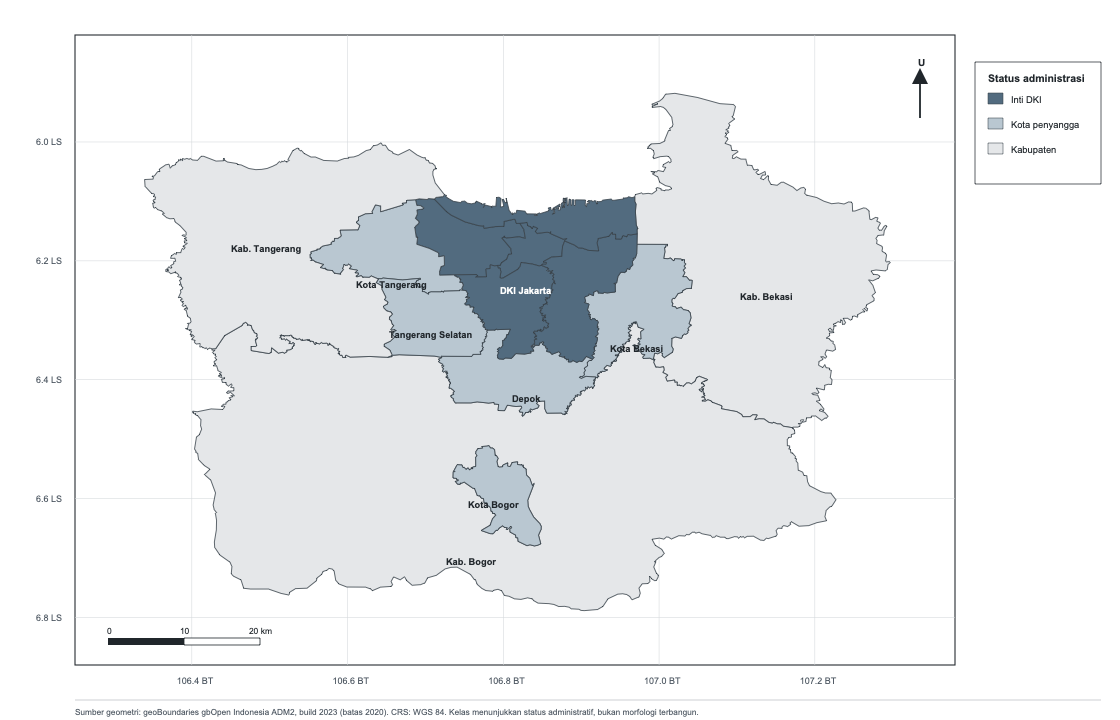
\includegraphics[width=0.98\textwidth]{bab4_status_administratif.png}
  \caption{Batas dan status administratif wilayah penelitian (gambar sementara). Sumber geometri: geoBoundaries gbOpen Indonesia ADM2, build 2023 dengan batas tahun 2020 \parencite{geoboundaries2023}. Kelas membedakan inti DKI, kota, dan kabupaten untuk pelaporan; kelas tersebut bukan ukuran morfologi atau kematangan pusat. Peta final memakai proyeksi UTM 48S dan memuat kabupaten tetangga, termasuk Cianjur, sebagai konteks.}
  \label{fig:bab4-status-administratif}
\end{figure}

Batas administrasi dipakai untuk menempatkan hasil pada kewenangan yang sesuai. Hubungan ekonomi, perjalanan, dan pelayanan dapat melintasi garis tersebut. Geometri ADM2 hanya dipakai untuk peta konteks. Analisis tingkat kecamatan memakai batas kecamatan BPS (Bab 3).

\section{Demografi dan massa lokal}

Pada 2024 penduduk Jabodetabek berjumlah sekitar 32,3 juta jiwa. Sekitar 21,6 juta di antaranya, atau 66,9 persen, tinggal di luar DKI Jakarta (Tabel \ref{tab:bab4-populasi}). Kabupaten Bogor merupakan unit berpenduduk terbesar di luar DKI, dengan 5,68 juta jiwa. Kepadatan sangat berbeda antara kota dan kabupaten. Kota Bekasi dan Kota Tangerang memiliki lebih dari 11.000 jiwa/km², sedangkan Kabupaten Bogor di bawah 1.900 jiwa/km².

\begin{table}[H]
\centering
\caption{Penduduk, kepadatan, dan jumlah kecamatan wilayah penelitian, 2024}
\label{tab:bab4-populasi}
\begin{tabularx}{\textwidth}{>{\raggedright\arraybackslash}X >{\raggedleft\arraybackslash}p{0.17\textwidth} >{\raggedleft\arraybackslash}p{0.17\textwidth} >{\raggedleft\arraybackslash}p{0.13\textwidth}}
\toprule
Unit administratif & Penduduk (ribu jiwa) & Kepadatan (jiwa/km²) & Kecamatan \\
\midrule
DKI Jakarta & 10.684,95 & 16.165 & 44 \\
Kabupaten Bogor & 5.682,30 & 1.899 & 40 \\
Kota Bogor & 1.078,35 & 9.683 & 6 \\
Kota Depok & 2.163,64 & 10.823 & 11 \\
Kabupaten Bekasi & 3.273,87 & 2.617 & 23 \\
Kota Bekasi & 2.644,06 & 12.411 & 12 \\
Kabupaten Tangerang & 3.400,49 & 3.309 & 29 \\
Kota Tangerang & 1.963,97 & 11.012 & 13 \\
Kota Tangerang Selatan & 1.399,50 & 8.489 & 7 \\
\midrule
Bodetabek (di luar DKI) & 21.606,18 & -- & 141 \\
\bottomrule
\end{tabularx}
\smallskip
\parbox{\textwidth}{\footnotesize Catatan: penduduk adalah proyeksi pertengahan tahun 2024 hasil SP2020. Kepadatan dibulatkan dari publikasi; dasar luas wilayah berbeda antartahun, sehingga kepadatan tidak dibandingkan dengan tahun lain. Jumlah kecamatan menurut kode wilayah BPS pada Lampiran 13 WSM 2024 (DKI termasuk dua kecamatan Kepulauan Seribu). Sumber: \textcite{bpsdki2025}, Tabel 3.1.1; \textcite{bpsjabar2025}, Tabel 3.1.1; \textcite{bpsbanten2025}, Tabel 3.1.1; \textcite{bpswsm2024}.}
\end{table}

Pada tingkat kecamatan, penduduk 141 kecamatan non-DKI berkisar dari sekitar 28 ribu jiwa (Bojongmangu, Kabupaten Bekasi) hingga 428 ribu jiwa (Tambun Selatan, Kabupaten Bekasi), dengan median sekitar 135 ribu jiwa \parencite[Lampiran 3]{bpswsm2024}. Kepadatan berkisar dari 277 jiwa/km² (Muara Gembong) hingga sekitar 18.900 jiwa/km² (Bekasi Barat). Rentang yang lebar ini menjadi alasan fungsi dibandingkan terhadap massa, bukan dibaca secara absolut. Jumlah penduduk kecamatan untuk tiga unit Banten pada lampiran tersebut berbeda 2--3 persen dari proyeksi kabupaten/kota, sehingga basisnya perlu dicek sebelum dipakai.

\begin{figure}[H]
  \centering
  \GambarPlaceholder{Peta kepadatan penduduk per kecamatan, 2024.\\
    Berkas target: \texttt{figures/bab4\_kepadatan\_kecamatan.pdf}}
  \caption{Kepadatan penduduk per kecamatan di Jabodetabek. Sumber: \textcite[Lampiran 3]{bpswsm2024}; batas kecamatan \textcite{hdxcodab2020}.}
  \label{fig:bab4-kepadatan}
\end{figure}

\section{Struktur ekonomi}

Struktur ekonomi kabupaten/kota di sekitar Jakarta sangat beragam (Tabel \ref{tab:bab4-pdrb}). Industri pengolahan menyumbang 77 persen PDRB Kabupaten Bekasi dan 52 persen PDRB Kabupaten Bogor, tetapi hanya 8 persen PDRB Kota Tangerang Selatan. Perdagangan memiliki pangsa sekitar seperlima di Kota Bogor, Kota Depok, dan Kota Bekasi. Kota Tangerang menonjol pada transportasi dan pergudangan, dengan pangsa sekitar sepertiga PDRB pada 2024. Di DKI Jakarta, perdagangan menyumbang 18 persen, sedangkan industri pengolahan dan jasa keuangan masing-masing sekitar 11 persen \parencite{bpsdki2026}.

\begin{table}[H]
\centering
\caption{PDRB atas dasar harga berlaku dan pangsa sektor terpilih menurut kabupaten/kota, 2024}
\label{tab:bab4-pdrb}
\begin{adjustbox}{max width=\textwidth}
\begin{tabular}{>{\raggedright\arraybackslash}p{0.27\textwidth} >{\raggedleft\arraybackslash}p{0.12\textwidth} >{\raggedleft\arraybackslash}p{0.13\textwidth} >{\raggedleft\arraybackslash}p{0.12\textwidth} >{\raggedleft\arraybackslash}p{0.12\textwidth} >{\raggedleft\arraybackslash}p{0.12\textwidth}}
\toprule
Unit & PDRB (triliun Rp) & Per kapita (juta Rp) & Industri pengolahan (\%) & Perdagangan (\%) & Transportasi dan pergudangan (\%) \\
\midrule
DKI Jakarta & 3.709,9 & 347,2 & 11,5 & 18,0 & 4,5 \\
Kabupaten Bogor & 311,7 & 54,9 & 51,7 & 12,3 & 4,7 \\
Kota Bogor & 61,1 & 56,6 & 18,4 & 19,1 & 14,0 \\
Kota Depok & 94,2 & 43,5 & 29,2 & 21,0 & 4,8 \\
Kabupaten Bekasi & 421,3 & 128,7 & 77,0 & 5,7 & 1,6 \\
Kota Bekasi & 129,4 & 48,9 & 33,1 & 20,7 & 13,0 \\
Kabupaten Tangerang & 186,1 & 54,7 & 33,7 & 11,4 & 3,6 \\
Kota Tangerang & 224,8 & 114,5 & 27,0 & 10,4 & 32,6 \\
Kota Tangerang Selatan & 112,2 & 80,2 & 8,1 & 16,7 & 3,7 \\
\bottomrule
\end{tabular}
\end{adjustbox}
\smallskip
\parbox{\textwidth}{\footnotesize Catatan: angka 2024 berstatus sangat sementara. PDRB dan PDRB per kapita dari \textcite{bpspdrb2025}; nilai DKI adalah jumlah kabupaten/kota. Pangsa sektor dari Tabel 12.3 \emph{Dalam Angka 2025} setiap kabupaten/kota \parencite{bpskabbogor2025,bpskotabogor2025,bpsdepok2025,bpskabbekasi2025,bpskotabekasi2025,bpskabtangerang2025,bpskotatangerang2025,bpstangsel2025}; pangsa DKI dari Tabel 13.1.3 \textcite{bpsdki2026}, karena tabel yang sama pada edisi 2025 memuat baris yang bergeser. PDRB per kapita mengukur nilai tambah menurut lokasi produksi, bukan pendapatan penduduk.}
\end{table}

PDRB per kapita yang tinggi di Kabupaten Bekasi dan Kota Tangerang sejalan dengan besarnya pangsa industri pengolahan di Kabupaten Bekasi serta transportasi dan pergudangan di Kota Tangerang. Angka ini mengukur nilai tambah menurut lokasi produksi, bukan pendapatan penduduk setempat. Sebaliknya, PDRB per kapita Kota Depok dan Kota Bekasi relatif rendah meskipun penduduknya besar. Pola ini konsisten dengan peran keduanya sebagai kawasan hunian yang penduduknya banyak bekerja di luar wilayahnya, tetapi belum membuktikan defisit fungsi.

\section{Pola komuter}

Survei Komuter Jabodetabek 2023 mencatat sekitar 4,41 juta komuter antarkabupaten/kota berumur 5 tahun ke atas, atau 14,9 persen penduduk kelompok umur tersebut. Sebanyak 3,61 juta di antaranya bekerja dan 0,80 juta bersekolah, kuliah, atau kursus. Komuter terbanyak bertempat tinggal di Kabupaten Bogor, yaitu 584 ribu orang, dengan 460 ribu di antaranya bekerja \parencite[Tabel 1 dan 4]{bpskomuter2023}.

Dari sekitar 2,85 juta komuter yang tinggal di Bodetabek, 53,0 persen menuju DKI Jakarta dan 44,6 persen menuju kabupaten/kota Bodetabek lain. Arus balik dari DKI ke Bodetabek sekitar 372 ribu orang. Orientasi ke DKI sangat berbeda antarunit (Tabel \ref{tab:bab4-komuter}). Lebih dari dua pertiga komuter Kota Depok, Kota Tangerang Selatan, dan Kota Bekasi menuju DKI. Sebaliknya, komuter Kabupaten Bogor, Kota Bogor, dan Kabupaten Tangerang lebih banyak bergerak antarpinggiran. Arus terbesar Kabupaten Bogor menuju Kota Bogor (142 ribu) dan Kota Depok (93 ribu). Kota Bogor dan Kota Tangerang Selatan menerima komuter masuk sebanyak atau lebih banyak daripada komuter keluarnya.

\begin{table}[H]
\centering
\caption{Komuter kabupaten/kota Bodetabek: arus 2023 dan orientasi ke DKI Jakarta, 2014--2023}
\label{tab:bab4-komuter}
\begin{adjustbox}{max width=\textwidth}
\begin{tabular}{>{\raggedright\arraybackslash}p{0.25\textwidth} >{\raggedleft\arraybackslash}p{0.11\textwidth} >{\raggedleft\arraybackslash}p{0.11\textwidth} >{\raggedleft\arraybackslash}p{0.10\textwidth} >{\raggedleft\arraybackslash}p{0.08\textwidth} >{\raggedleft\arraybackslash}p{0.08\textwidth} >{\raggedleft\arraybackslash}p{0.08\textwidth} >{\raggedleft\arraybackslash}p{0.10\textwidth}}
\toprule
 & \multicolumn{3}{c}{2023} & \multicolumn{3}{c}{Ke DKI (\% komuter keluar)} & \\
\cmidrule(lr){2-4}\cmidrule(lr){5-7}
Tempat tinggal & Komuter keluar & Ke Bodetabek lain (\%) & Komuter masuk & 2014 & 2019 & 2023 & Rasio masuk/ keluar 2023 \\
\midrule
Kabupaten Bogor & 584.041 & 63,8 & 186.886 & 32,0 & 36,4 & 32,3 & 0,32 \\
Kota Bogor & 130.470 & 73,0 & 159.555 & 38,7 & 22,5 & 26,0 & 1,22 \\
Kota Depok & 485.355 & 23,1 & 217.410 & 79,0 & 75,0 & 76,5 & 0,45 \\
Kabupaten Bekasi & 333.484 & 49,2 & 153.885 & 52,2 & 47,3 & 43,3 & 0,46 \\
Kota Bekasi & 466.260 & 29,2 & 258.759 & 78,1 & 74,3 & 68,2 & 0,55 \\
Kabupaten Tangerang & 279.111 & 69,6 & 144.977 & 29,0 & 29,5 & 28,8 & 0,52 \\
Kota Tangerang & 327.220 & 40,7 & 274.102 & 68,0 & 73,6 & 58,7 & 0,84 \\
Kota Tangerang Selatan & 239.984 & 25,1 & 244.908 & 83,4 & 80,7 & 74,5 & 1,02 \\
\midrule
Bodetabek & 2.845.925 & 44,6 & -- & 61,1 & 58,0 & 53,0 & -- \\
\bottomrule
\end{tabular}
\end{adjustbox}
\smallskip
\parbox{\textwidth}{\footnotesize Catatan: dihitung dari Tabel 2 (matriks asal-tujuan) setiap edisi. Komuter keluar adalah arus ke kabupaten/kota lain di Jabodetabek dan ke luar Jabodetabek; sisa persentase setelah DKI dan Bodetabek lain adalah arus ke luar Jabodetabek. Komuter masuk dihitung dari seluruh tempat tinggal di Jabodetabek, termasuk DKI. Rumusan definisi komuter edisi 2023 berbeda dari edisi 2014 dan 2019, dan bulan pencacahan serta kerangka sampelnya juga berbeda. Sumber: \textcite{bpskomuter2014,bpskomuter2019,bpskomuter2023}.}
\end{table}

Ketiga edisi survei memperlihatkan pangsa komuter Bodetabek yang menuju DKI menurun dari 61,1 persen pada 2014 menjadi 58,0 persen pada 2019 dan 53,0 persen pada 2023. Pangsa arus antarpinggiran naik dari 36,1 persen menjadi 39,4 persen dan 44,6 persen. Jumlah komuter tercatat 3,57 juta pada 2014, 3,26 juta pada 2019, dan 4,41 juta pada 2023. Perbedaan rumusan definisi, bulan pencacahan, dan kerangka sampel antaredisi membuat angka ini dibaca sebagai arah perubahan estimasi survei, bukan besaran perubahan yang pasti.

Beban perjalanan juga tidak merata. Pada 2023, 14,4 persen komuter Jabodetabek menempuh perjalanan berangkat sedikitnya 90 menit, dan 28,6 persen mengeluarkan biaya transportasi pergi-pulang sedikitnya Rp25.000 per hari \parencite[Tabel 20 dan 35]{bpskomuter2023}. Rincian per kabupaten/kota asal, bersama distribusi penghasilan komuter, dianalisis pada Bab 5 sebagai profil beban dan manfaat.

Pada tingkat kecamatan, persentase komuter menuju kawasan inti WSM berkisar dari 1,9 persen hingga 47,8 persen. Dari 141 kecamatan non-DKI, 105 termasuk kawasan inti, 27 termasuk periferi, dan 9 kecamatan di Kabupaten Bogor tidak termasuk wilayah metropolitan statistik \parencite[Lampiran 13]{bpswsm2024}. Seluruh kecamatan Kota Bogor, Kota Depok, Kota Bekasi, Kota Tangerang, dan Kota Tangerang Selatan termasuk kawasan inti.

\begin{figure}[H]
  \centering
  \GambarPlaceholder{Peta alir komuter antarkabupaten/kota, 2023.\\
    Berkas target: \texttt{figures/bab4\_komuter\_od\_2023.pdf}}
  \caption{Arus komuter antarkabupaten/kota di Jabodetabek, 2023. Sumber: \textcite[Tabel 2]{bpskomuter2023}.}
  \label{fig:bab4-komuter-od}
\end{figure}

\begin{figure}[H]
  \centering
  \GambarPlaceholder{Peta persentase komuter menuju kawasan inti per kecamatan, 2024.\\
    Berkas target: \texttt{figures/bab4\_komuter\_ke\_inti\_kecamatan.pdf}}
  \caption{Persentase komuter menuju Kawasan Inti Perkotaan 1 per kecamatan, Agustus 2024. Kawasan inti WSM lebih luas daripada DKI Jakarta. Sumber: \textcite[Lampiran 13]{bpswsm2024}.}
  \label{fig:bab4-komuter-inti}
\end{figure}

\section{Morfologi terbangun dan jaringan transportasi}

Morfologi Jabodetabek terbentuk dari inti perkotaan padat, koridor jalan dan rel, kawasan industri, perumahan berskala besar, serta ruang terbuka yang tersisa di antaranya. Studi tentang dekonsentrasi manufaktur dan perluasan jalan tol menunjukkan bahwa perkembangan tersebut tidak seragam antarwilayah \parencite{hudalahetal2013,pratamaetal2022}. Volume terbangun total dan nonhunian dari GHSL R2023A memperlihatkan potret kapasitas fisik tersebut \parencite{ghsl2023builtv}. Data epoch 2020 merupakan hasil interpolasi dengan observasi terdekat 2018, sehingga dibaca sebagai potret, bukan perubahan.

\begin{figure}[H]
  \centering
  \GambarPlaceholder{Peta volume terbangun total dan nonhunian (GHSL R2023A, epoch 2020).\\
    Berkas target: \texttt{figures/bab4\_terbangun\_nonhunian.pdf}}
  \caption{Volume terbangun total dan nonhunian di Jabodetabek, epoch 2020 hasil interpolasi dengan observasi terdekat 2018. Sumber: \textcite{ghsl2023builtv}.}
  \label{fig:bab4-terbangun}
\end{figure}

Jaringan transportasi memberi jalur bagi hubungan metropolitan, tetapi keberadaan jaringan tidak sama dengan penggunaannya. Jaringan yang beroperasi meliputi KRL Commuter Line, MRT Jakarta, LRT Jabodebek, TransJakarta, dan jalan tol, sedangkan JUTPI 3 menyusun usulan jaringan angkutan umum dengan horizon 2045 \parencite{jica2025jutpi}. Pada peta final, jaringan eksisting dari OSM dan GTFS TransJakarta digambar dengan garis penuh dan rencana 2045 dengan garis putus. Peta usulan JUTPI 3 di bawah dipakai sementara sebagai konteks kebijakan.

\begin{figure}[H]
  \centering
  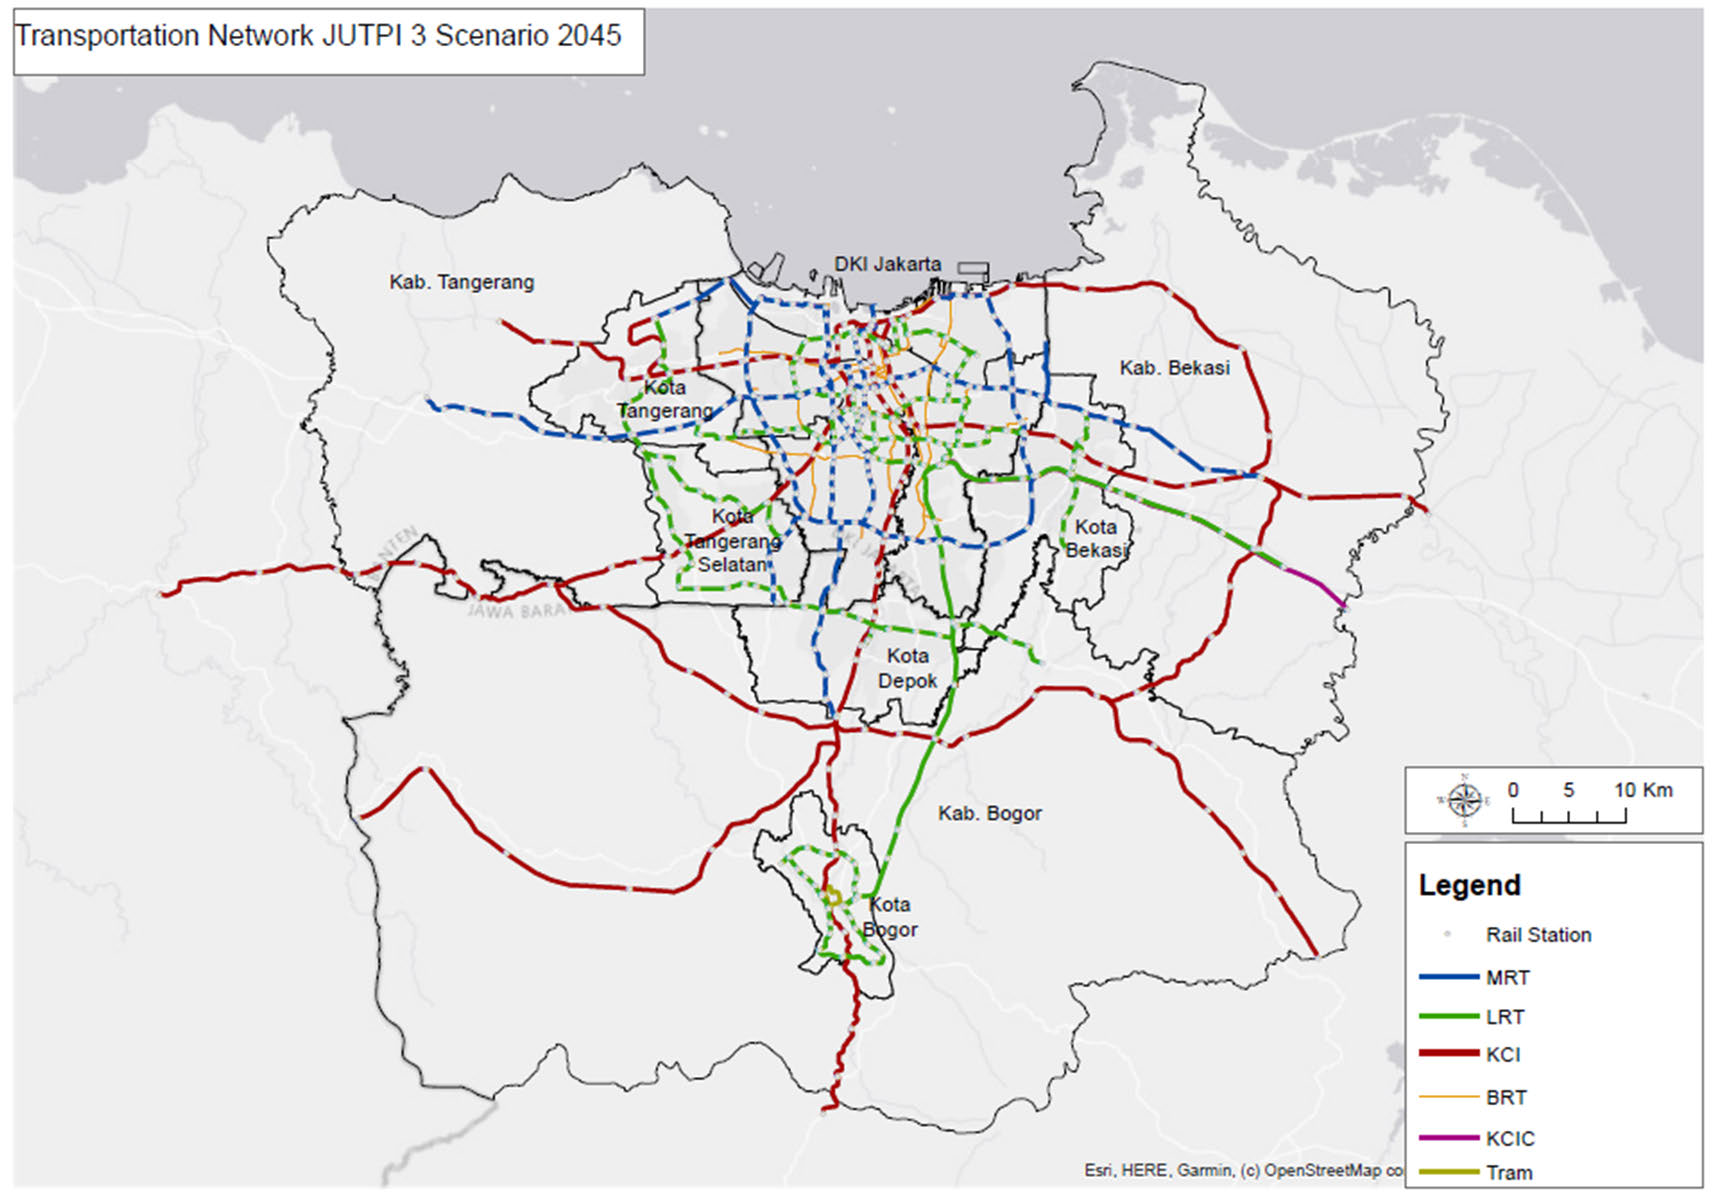
\includegraphics[width=0.90\textwidth]{bab4_network_jutpi.png}
  \caption{Peta jaringan angkutan umum masa depan yang diusulkan JUTPI 3 untuk Jabodetabek (gambar sementara). Sumber: JICA Expert Team dalam \emph{Project Completion Report} 2025 \parencite{jica2025jutpi}. Peta dibaca sebagai skenario kebijakan, bukan jaringan yang beroperasi atau arus aktual.}
  \label{fig:bab4-network}
\end{figure}

\section{Kawasan industri dan kota baru}

Data kawasan industri Kementerian Perindustrian 2025 memuat 21 kawasan industri formal di Jabodetabek \parencite{kemenperin2025ki}. Sepuluh kawasan berada di Kabupaten Bekasi, antara lain MM2100, Jababeka, Greenland International Industrial Center, Lippo Cikarang, dan East Jakarta Industrial Park. Enam kawasan berada di Kabupaten Tangerang, dua di Kabupaten Bogor, dan masing-masing satu di Jakarta Timur, Jakarta Utara, serta Kota Tangerang Selatan. Kota Bogor, Kota Depok, Kota Bekasi, dan Kota Tangerang tidak memiliki kawasan industri formal dalam data tersebut. Kawasan industri formal hanya sebagian dari kegiatan manufaktur, dan data ini tidak memuat jumlah tenant atau tenaga kerja.

Kota baru swasta berskala besar, seperti Bumi Serpong Damai (BSD), Lippo Karawaci, Lippo Cikarang, Jababeka, dan Sentul, membentuk pusat hunian, perdagangan, dan jasa di luar inti \parencite{firman2004,firmanfahmi2017}. Kawasan industri dan kota baru diperlakukan sebagai penjelasan alternatif bagi fungsi relatif (Bab 3), bukan sebagai bukti kematangan pusat.

\begin{figure}[H]
  \centering
  \GambarPlaceholder{Peta kawasan industri formal dan kota baru skala besar.\\
    Berkas target: \texttt{figures/bab4\_kawasan\_industri.pdf}}
  \caption{Kawasan industri formal dan kota baru skala besar di Jabodetabek. Sumber: \textcite{kemenperin2025ki}; lokasi kota baru dari OSM dan literatur.}
  \label{fig:bab4-industri}
\end{figure}

\section{Pusat sekunder berbasis massa}

Pusat sekunder ditandai dengan aturan massa yang ditetapkan pada Bab 3, yaitu kuartil teratas penduduk atau volume terbangun hunian di antara 141 kecamatan non-DKI. Berdasarkan penduduk saja, ambang kuartil teratas adalah sekitar 194 ribu jiwa, dan 36 kecamatan melampauinya. Delapan di antaranya berada di Kota Bekasi, tujuh di Kabupaten Bekasi, enam di Kabupaten Bogor, lima di Kota Depok, tiga masing-masing di Kota Bogor, Kabupaten Tangerang, dan Kota Tangerang Selatan, dan satu di Kota Tangerang \parencite[dihitung dari Lampiran 3]{bpswsm2024}. Daftar akhir ditetapkan setelah kriteria volume terbangun hunian dihitung dan basis penduduk kecamatan Banten diperiksa. Penandaan ini tidak memakai fungsi, kawasan industri, atau arus, sehingga kecamatan hunian berpenduduk besar ikut terpilih.

\begin{figure}[H]
  \centering
  \GambarPlaceholder{Peta kecamatan yang ditandai sebagai pusat sekunder berbasis massa.\\
    Berkas target: \texttt{figures/bab4\_pusat\_berdasarkan\_massa.pdf}}
  \caption{Kecamatan non-DKI yang ditandai sebagai pusat sekunder berbasis massa. Sumber: penduduk dari \textcite[Lampiran 3]{bpswsm2024}; volume terbangun hunian dari \textcite{ghsl2023builtv}; ambang dari Bab 3.}
  \label{fig:bab4-pusat-massa}
\end{figure}

\section{Audit sumber dan periode}

Tabel \ref{tab:bab4-audit} menghubungkan gambaran lokasi dengan metode pengukuran. Tahun pada tabel adalah tahun observasi, tahun proyeksi, tahun geometri, atau tahun publikasi sesuai keterangan. Satu baris tidak dipakai untuk menyiratkan seri waktu yang tidak ada.

\begingroup
\footnotesize
\setlength{\tabcolsep}{4pt}
\begin{longtable}{>{\raggedright\arraybackslash}p{0.19\textwidth} >{\raggedright\arraybackslash}p{0.21\textwidth} >{\raggedright\arraybackslash}p{0.14\textwidth} >{\raggedright\arraybackslash}p{0.38\textwidth}}
\caption{Audit sumber dan periode untuk Bab 4}\label{tab:bab4-audit}\\
\toprule
Konstruk/lapisan & Sumber & Tahun/periode & Status bukti dan batas penggunaan \\
\midrule
\endfirsthead
\caption[]{Audit sumber dan periode untuk Bab 4 (lanjutan)}\\
\toprule
Konstruk/lapisan & Sumber & Tahun/periode & Status bukti dan batas penggunaan \\
\midrule
\endhead
\midrule
\multicolumn{4}{r}{\footnotesize Dilanjutkan pada halaman berikutnya}\\
\endfoot
\bottomrule
\endlastfoot
Kebijakan & UU 2/2024; Perpres 60/2020 & 2024; 2020 & Norma hukum dan rencana; bukan observasi kondisi \parencite{uu22024,perpres602020}. \\
Batas administratif & geoBoundaries ADM2; batas kecamatan COD-AB HDX & Build 2023; batas 2020 & Geometri konteks dan agregasi; tidak menetapkan batas fungsional. \\
Penduduk dan kepadatan kab/kota & \emph{Dalam Angka 2025} provinsi DKI, Jawa Barat, dan Banten & Proyeksi 2024 & D pada tingkat kab/kota; dasar luas berubah antartahun. \\
Penduduk dan luas kecamatan & WSM 2024, Lampiran 3 & \emph{Dalam Angka 2024}; peta BPS 2024 & D; jumlah kecamatan Banten perlu dicocokkan dengan proyeksi kab/kota. \\
Struktur ekonomi & PDRB kab/kota 2020--2024; \emph{Dalam Angka 2025} kab/kota & 2024 (sangat sementara) & A untuk penelitian berkecamatan; konteks. \\
Komuter & Statistik Komuter Jabodetabek & 2014, 2019, 2023 & D pada 13 kab/kota; definisi dan desain sampel berbeda antaredisi. \\
Integrasi kecamatan & WSM 2024, Lampiran 13 & MPD Agustus 2024 & A; tujuan arus adalah kawasan inti morfologis, bukan DKI saja. \\
Volume terbangun & GHSL GHS-BUILT-V R2023A & Epoch 2020 (interpolasi) & P; potret kapasitas fisik, bukan perubahan. \\
Kawasan industri & Kemenperin, 125 KI & 2025 & D untuk kawasan formal; satuan luas belum terdokumentasi. \\
Jaringan & OSM; GTFS TransJakarta; JUTPI 3 & 2026; 2026; usulan 2045 & Eksisting dipisahkan dari rencana. \\
\end{longtable}
\endgroup

\section{Batas interpretasi gambaran lokasi}

Bab ini menyediakan batas administratif untuk pemetaan, gambaran massa lokal dan struktur ekonomi untuk membaca perbedaan antarunit, serta gambaran pola komuter sebagai konteks pengukuran relasi. Ketiganya menjadi konteks bagi pengukuran, bukan hasil diagnosis.

Penurunan orientasi ke DKI dan kenaikan arus antarpinggiran belum menunjukkan bahwa pusat sekunder telah matang. Arus antarpinggiran dapat mencerminkan pusat kerja industri, akses layanan, atau sekadar persebaran permukiman. Demikian pula, PDRB per kapita yang tinggi tidak menunjukkan fungsi layanan yang kuat. Bab 5 menguji apakah fungsi relatif setiap kecamatan berhubungan dengan integrasinya, dan apakah pola tersebut lebih dekat dengan \emph{borrowed size}, \emph{agglomeration shadow}, campuran keduanya, atau hasil yang belum terselesaikan.

\printbibliography[heading=bibintoc,title={Daftar Pustaka}]
\end{document}
